%!TEX root = ../dissertation.tex

\chapter{Analyzing Color Mixing Perception}
\label{chapter:results}
%
In this section, we are going to dive into the results obtained from the user study described on chapter number \ref{chapter:design}.
On the first section, we will clearly explain the test protocol which was followed by the users in the laboratory environment to correctly
execute the study; this section will be followed, not only by the description of how the gathered data was treated and cleaned
(Section \ref{sec:results_datacleaning}), but also the transformation of this data using \emph{Matlab} processing tools, in order to prepare
it for the statistical scrutiny (Section \ref{sec:results_digest}). Hereafter, conclusions will be drawn from the study at section
\ref{sec:results_results}, when trying to find answers to the questions/objectives raised before. \par
%
The final section of this chapter will be dedicated to summarize the results and infer important conclusions, implications and guidelines which
could be relevant for the InfoVis field of research.
%%%%%%%%%%%%%%%%%%%%%%%%%%%%%%%%%%%%%%%%%%%%%%%%%%%%%%%%%%%%%%%%%%%%%%%%%%%%%%%%%%%%%%%%%%%%%%%%%%%%%%%%%%%%%%%%%%%%%%%%%%%%%%%%%%%%%%%%%%%%%%%%%%%
%                                                                PROTOCOL                                                                         %
%%%%%%%%%%%%%%%%%%%%%%%%%%%%%%%%%%%%%%%%%%%%%%%%%%%%%%%%%%%%%%%%%%%%%%%%%%%%%%%%%%%%%%%%%%%%%%%%%%%%%%%%%%%%%%%%%%%%%%%%%%%%%%%%%%%%%%%%%%%%%%%%%%%
\section{Protocol}
\label{sec:results_protocol}
%
The existence of a test protocol, when performing a User Study is mandatory: without it, the test may not follow a strictly previously defined
standard. As written before, this user study was conducted two-pronged: in a laboratory environment and \emph{via} online dissemination channels. \par
%
\subsection{Laboratory Environment}
%
The users were given always the same briefing when they arrived at the user study test site: it was explained the motivation behind the master
thesis, the goals which were expected for this phase of the study and what was expected for them to execute. The most important information which
was told was that \ul{"there was no pre-defined correct and wrong answers to each question, this test was designed to test the general
color mixing capabilities of the majority of the users"}. Besides this information, the user study was self-contained, in the sense that
every other relevant information and instruction was in the interface, adapted for each test phase, so it was not given any physical artifacts
describing instructions. The instructions were available on two languages, depending on the choice of the user: Portuguese and English. \par
%
Before each session of the laboratory environment test-run, a Datacolor Spyder 5 Elite Color Calibrator was USB-connected to the computer and, using
the software which is shipped along with it, the computer LCD display was fully calibrated (the software offers the option of recalibrating,
the option of checking the calibration and also, the option of fully calibrating the display) by testing the pixel emission when emmiting a particular
set of colors. The display was everytime fully calibrated, since the software manisfested an erratic bahaviour when using the other functions:
the screen colors were presented in a very warmer/colder color profile tha it was before. \par
%
The tests were conducted at, most of the repetitions, in \gls{RNL} at \gls{IST}, and fewers times in other locations with similar conditions:
this is due to constraints in finding users, so the test site needed to have a (limited) mobility feature. However, the conditions remained
the same concerning the illumination, the position of the user and the computer used: a Macbook Air 13' (Mid-2013) was prepared undeneath
a fixed incadescent light-source (but slightly deviated from it, to minimize light reflections on screen), the user would sit in front
of the laptop, in an almost silent environment. Ideal conditions of this test would be such that the user could be sitting alone in a completely
silent room, his head would be always at the same distance from the screen, resting in a head-rest and the LCD display's inclination would be perfectly
adjusted to the user's eyes. \par
%
\subsection{Online Environment}
%
Performing the study online, as easily predictable, develops some characteristics which cannot be completly controlled. For the sake of calibration, it was asked the user
to perform a set of six calibration easy steps before starting the test, so the online user's screen would be,
somehow, in a standardized calibration fashion. The calibration steps which were asked are:
%
\begin{enumerate}
  \item If possible, adjust your room lights for a comfortable usage of your device.
  \item Avoid reflections on your screen, by diverting the screen from direct sources of light. This step is important,
  since light reflections can affect visualization of images.
  \item To adjust the \textbf{Black Point} of your screen, define the \ul{Contrast} and \ul{Brightness} of your screen to their maximum.
  \item After Step 3, gradually reduce \textbf{Brightness} value of your screen, in order to correctly distinguish the squares of each image below [calibration squares images].
  \item If possible, define the \textbf{Color Temperature} of your screen to 6500 Kelvin Degrees.
  \item You are now ready to answer the following questions!
\end{enumerate} \par
%
The ideal conditions of this test would be such that we could control and maniupulate the color calibration of online user's LCD display, using a software
piece which would acquire important informations from the screen configuration, \emph{e.g.} resolution, white-point, black-point, brightness, among others,
digest the values and present the questions from the Core Phase in a completely controled and calibrated window. Further investigation could focus in
developing this system. \par
%
The users were asked to fill in a profiling questionnaire (as seeen of section \ref{subsec:design_profiling}), as well as to respond to calibration form
(Section \ref{subsec:design_calibration}). A validated simplified 6-plate Ishihara color blindness test \cite{Alwis1992} is, then performed
(Section \ref{subsec:design_ishihara}), before proceeding onto the 32 questions test-phase, in which the user is asked to slide one(two) circular
object(s) placed on top of a bar, to indicate a(the) color(s) which he thought were the correct mixture answers. In the end, the user could leave
feedback, by sending a message which would be stored in a Relational Database. \par
%
The instructions which were presented in each page can be consulted in Appendix \ref{appendix:protocol}. \par
%
%%%%%%%%%%%%%%%%%%%%%%%%%%%%%%%%%%%%%%%%%%%%%%%%%%%%%%%%%%%%%%%%%%%%%%%%%%%%%%%%%%%%%%%%%%%%%%%%%%%%%%%%%%%%%%%%%%%%%%%%%%%%%%%%%%%%%%%%%%%%%%%%%%%
%                                                                DATA CLEANING                                                                    %
%%%%%%%%%%%%%%%%%%%%%%%%%%%%%%%%%%%%%%%%%%%%%%%%%%%%%%%%%%%%%%%%%%%%%%%%%%%%%%%%%%%%%%%%%%%%%%%%%%%%%%%%%%%%%%%%%%%%%%%%%%%%%%%%%%%%%%%%%%%%%%%%%%%
\section{Data Cleaning}
\label{sec:results_datacleaning}
%
Throughout the user study, we collected a \textbf{total amount of four-hundred and seventy-nine (477) users} which interacted with our study and fulfilled,
at least, until the Color Vision Deficiencies Test Phase. However, only \textbf{two-hundred and sixty-one (259) users went on to the core phase of the study},
representing \textbf{54.29\%} of the total amount, giving at least one answer on the set of 32 questions, loosing the other two hundred and eighteen
(218) users which did not leave any answer, defining the remaining percentage \textbf{45.71\%}. This large drop of users could be due to errors
reported by the users, apparently the inability to submit answers when using the "Submit" button after rating the question; there were also some complaints
when users tried to perform the study in some mobile devices (namely, the \emph{iPhone\textsuperscript{\textregistered} 6}), whereon the color slider was
not able to be dragged and change the color value at the user will. \par
%
Concerning the percentage of users which showed up at the \textbf{laboratory trials, there were twenty-nine (28) users who performed the entire study}.
On the other hand, there were \textbf{two-hundred and thirty-two (231) users which carried out the study online}. There was also a small sample of color vision
deficient users which we will analyze in a qualitative manner; this set of users contains only one (1) user from the Laboratory Environment - \textbf{3.57\%} of
the sample size - and two (2) online users - \textbf{less than 1\%}. Lastly, we detected a small percentage of \textbf{six (6) users (2.59\%) which did not
presented a correct calibration of its LCD display}, evaluation based on the criteria referred before.
%
The data presented and used in this dissertation document was gathered along roughly two months, from 15th of April until 8th of June. As said before,
it was collected both with online and laboratory users, which was therefore stored in a Relational Database as previously explained in section
\ref{sec:impl_designingsolution}. \par
%
In the end of the study, \gls{CSV} files were exported from each table using a PostgreSQL for macOS called
\emph{Postico}\footnote{Postico - a modern PostgreSQL client for the Mac, Available at: \url{eggerapps.at/postico/}. Last accessed on
September 11th, 2016.}, which originated five files containing raw data to be cleaned and processed. The files were as follows:
%
\begin{itemize}
  \item \emph{raw\_data\_user\_profile.csv} - Data aggregated from "Profiling", "Calibration" and "Color Vision Deficiencies" Tables;
  \item \emph{raw\_data\_first\_profiling.csv} - Data from "Profiling" Table;
  \item \emph{raw\_data\_first\_calibration.csv} - Data from "Calibration" Table;
  \item \emph{raw\_data\_first\_ishihara.csv} - Data from "Color Vision Deficiencies" Table;
  \item \emph{raw\_data\_first\_results.csv} - Data from "Results" Table;
\end{itemize} \par
%
\begin{table}[htbp]
  \resizebox{\textwidth}{!} {
  \begin{tabular} {|c|c|c|c|c|c|c|c|c|c|}
    \hline
    User ID & Type & First Color & Second Color & Third Color & Drags & Time & Rating & Resets & Question ID \\ \hline \hline
    5710cca334d60 & objTwoColors & \#0080FF & hsl(58.69565217391305,1,0.50) & hsl(98.15217391304348,1,0.50) & 992 & 117 & 4 & 2 & 10 \\ \hline
    5745c1c07cc0c & objTwoColors & \#8000FF & hsl(300,1,0.50) & hsl(324.13043478260875,1,0.50) & 645 & 55 & 2 & 1 & 14 \\ \hline
    5745350dc1e22 & objTwoColors & \#0080FF & hsl(226.30434782608697,1,0.50) & NONE & 115 & 11 & 5 & 1 & 10 \\ \hline
    57451c3b38192 & objTwoColors & \#00FF80 & NONE & hsl(150,1,0.50) & 462 & 39 & 5 & 1 & 15 \\ \hline
    574511e99b6d9 & objTwoColors & \#0080FF & hsl(15.652173913043478,1,0.50) & hsl(316.30434782608694,1,0.50) & 442 & 40, & 1 & 1 & 10 \\ \hline
    57427cf6bad0c & twoColorsObj & \#00FFFF & \#FFFF00 & \#46FF9C & 6 & 14 & 3 & 1 & 32 \\ \hline
    5740bda9be3dc & objTwoColors & \#FF7200 & hsl(9.130434782608695,1,0.50) & hsl(50.21739130434783,1,0.50) & 45 & 22 & 5 & 1 & 11 \\ \hline
    573c783748e8b & twoColorsObj & \#00FFFF & \#CBFF00 & \#00FF6B & 44 & 25 & 3 & 1 & 32 \\
    \hline
  \end{tabular}}
  \caption[Excerpt of Raw "Results" Table]{Excerpt of Results Table, with raw data.}
  \label{table:csv_resultsraw}
\end{table} \par
%
The refined tables were then divided into new and more specific ones so that we could detail our results analysis according to the goals defined before;
the "Results" table was refined into \ul{Laboratory Results}, \ul{Online Results} and demographic results: concerning the age, we divided it
on \ul{Users aged below 20 Years Results}, \ul{Users aged between 20 and 29 Years Results}, \ul{Users aged between 30 and 39 Years Results},
\ul{Users aged between 40 and 49 Years Results}, \ul{Users aged between 50 and 59 Years Results} and \ul{Users aged above 60 Years Results}.
Respecting the division of genders, we created the categories \ul{Female Users Results}, \ul{Male Users Results} and \ul{Other Gender Users Results}.
An excerpt of raw data contained in "Results" table can be found in table \ref{table:csv_resultsraw}; this allows us to support the explanation of the
following steps of the cleaning phase. \par
%
Dividing the results among smaller \gls{CSV} files was the first step of the cleaning phase: the next checklist represents the detailed path which
was followed to fulfill the data cleaning.
%
\begin{itemize}
  \item \textbf{Remove "hsl(..., 1, 0.50)"} - It was needed to remove the extra information stored in columns \emph{First Color, Second Color}
   and \emph{Third Color}, since this is redundant because it never varies from entry to entry of the table (remember Section \ref{sec:impl_objectives}).
   These values are the \emph{Saturation} (S) and \emph{Value} (V), primitives of the HSV Color Model used.
  \item \textbf{Format Values} - This step was performed just after the previous one. The value which remains to be formatted is simply the \emph{Hue} (H),
  which is equal to a very precise position on the coded color slider on the interface; the value was composed of 14 decimal numbers, giving us much more
  precision than what is, in fact, needed considering that the hue is measured in terms of integer numbers. The number was rounded up to its closest
  integer number, then. Besides that, there was still one value to be adjusted which was the missing response: \emph{NONE} neeeded to be
  replaced by 0, to simplify the processing of null answers.
  \item \textbf{Sort Entries} - In order to favour the iteration when processing the data, each line of the "Results" Table was
  sorted according, firstly to the \emph{Question ID}, and after by \emph{User ID}.
  \item \textbf{Normalize Laboratory Data} - As previously said, to perform the Laboratory Study we used a Spyder Color Calibrator to manage the color
  representation independently of the environmental conditions of light. Since the Color Profile file generated by the calibrator was used to adapt colors
  to be presented to the user, those same colors had to be trackbacked to the original color, for the sake of normalization of values. This is
  specially useful when comparing the results from this environment to the "Online" Results, helping in data processing later.
  \item \textbf{Verify Duplicated Entries} - This step was performed only to ensure that the entries would not have any matching copy. As expected,
  there were not found any copies.
  \item \textbf{Normalize Profiling Info} - Regarding the "Profiling" data, there was some which was written in Portuguese and other in English, depending on
  the language to perform the study chosen by the user. To avoid misleading profiling categories, all of the academic degrees were normalized to its corresponding
  name both in English and Portuguese. Also, the raw language values contained some specification of English dialects (\emph{e.g.} en\_US, en\_UK) and other languages,
  which was more information than we actually needed; these values were normalized to correspond only to its native and original language (like English, solely).
  \item \textbf{Sanitizing Users} - The tables contained many entries from users that performed the study with incorrect calibration and from users which
  gave unexpected values on the color deficiencies test phase; the entries which corresponded to a user that failed all 6 values on the later phase, would be
  deleted, leaving no trace of its participation. Concerning the bad calibration values, it "opened a window" to investigate the resilience of results when the
  calibration was not what it was expected - this will covered in sub-section \ref{subsec:results_calibration}. To end up the cleaning phase,
  it was decided to treat the color deficient users independently: we separated their values from the regular users to perform a qualitative evaluation.
\end{itemize} \par
%
An example of clean data can be found in table \ref{table:csv_resultsclean}. The next step of data handling is processing it to prepare metrics, establish comparations
to pre-calculated answers and depict results in a CIE Chromaticity Diagram. More tables can be found in Appendix \ref{appendix:tables}, specifically Section
\ref{appendix:sec_results}. \par
%
\begin{table}[htbp]
  \resizebox{\textwidth}{!} {
  \begin{tabular} {|c|c|c|c|c|c|c|c|c|c|}
    \hline
    User ID & Type & First Color & Second Color & Third Color & Drags & Time & Rating & Resets & Question ID \\ \hline \hline
    5713a02a13044 & objTwoColors & \#00FF00 & 0 & 137 & 459 & 56 & 2 & 0 & 17 \\ \hline
    573e4d0eb795b & objTwoColors & \#00FF00 & 235 & 59 & 121 & 28 & 4 & 0 & 17 \\ \hline
    573edae85268b & objTwoColors & \#00FF00 & 242 & 57 & 224 & 20 & 5 & 0 & 17 \\ \hline
    5740ad339507d & objTwoColors & \#00FF00 & 228 & 67 & 205 & 14 & 3 & 0 & 17 \\ \hline
    573c70dabcfe0 & objTwoColors & \#00FF00 & 55 & 221 & 192 & 14 & 2 & 0 & 17 \\ \hline
    57582b17cd76a & twoColorsObj & \#FF0000 & \#00FF00 & \#AF0049 & 724 & 65 & 2 & 0 & 18 \\ \hline
    573c783748e8b & twoColorsObj & \#FF0000 & \#00FF00 & \#BFBE00 & 656 & 47 & 3 & 0 & 18 \\ \hline
    573e4022949b1 & twoColorsObj & \#FF0000 & \#00FF00 & \#B000FF & 334 & 23 & 2 & 0 & 18 \\ \hline
    571151812791a & twoColorsObj & \#FF0000 & \#00FF00 & \#C9B2A2 & 110 & 39 & 2 & 0 & 18 \\
    \hline
  \end{tabular}}
  \caption[Excerpt of Clean "Results" Table]{Excerpt of Results Table, with clean data.}
  \label{table:csv_resultsclean}
\end{table}
%%%%%%%%%%%%%%%%%%%%%%%%%%%%%%%%%%%%%%%%%%%%%%%%%%%%%%%%%%%%%%%%%%%%%%%%%%%%%%%%%%%%%%%%%%%%%%%%%%%%%%%%%%%%%%%%%%%%%%%%%%%%%%%%%%%%%%%%%%%%%%%%%%%
%                                                              DATA PROCESSING                                                                    %
%%%%%%%%%%%%%%%%%%%%%%%%%%%%%%%%%%%%%%%%%%%%%%%%%%%%%%%%%%%%%%%%%%%%%%%%%%%%%%%%%%%%%%%%%%%%%%%%%%%%%%%%%%%%%%%%%%%%%%%%%%%%%%%%%%%%%%%%%%%%%%%%%%%
\section{Data Processing}
\label{sec:results_digest}
%
Processing the data was an important part of the process, since it was important to prepare the raw data collected and compute additional metrics which could be further
analyzed to answer the raised questions. To perform this processing, we decided to implement a set of scripts in \emph{Matlab} which could gauge the dataset of each question,
demographic group and subset of users (non-calibrated and color vision deficients). \par
%
With this data processing, we intend to verify each answer-pair given by a certain user and compare the pairs with each other. It was important to separate the results by question
ID, compare each questions' results with other questions that could conceive the same results, blend the values to check which color model answers are closer to (either \gls{HSV}, \gls{RGB},
\gls{CMYK}, CIE-L*a*b* or CIE-L*C*h*) and also, give meaning to each value, attributing a name to each color. All these parameters and computations are describred in the next two
sub-sections. \par
%
%\begin{lstlisting}[frame=single,basicstyle=\small,label={lst:pseudo_file},]
%  % Pseudo-codigo generico;
%  % Estrutura do ficheiro;
%\end{lstlisting}
%\captionof{lstlisting}{Pseudo-code representing each Script organization.}
%
\subsection{Data Preparation}
\label{subsec:results_preparation}
%
Given the fact that questions had some differences between each other, there would have to be a cautious analysis; to achieve this, we developed a script for each question, each of
file contains the particular set of characteristics ans specific comparisons and values of each question. An exemplary structure of these files can be found on pseudo-code box above.
Each question file is capable of computing the following datasets: \par
%
\begin{itemize}[noitemsep]
  \item Laboratory Results (Regular Users);
  \item Laboratory Results (Daltonic Users);
  \item Online Results (Regular Users);
  \item Online Results (Daltonic Users);
  \item Online Results (Uncalibrated Users);
  \item Demographic Groups: Users Aged Below 20 Years Results;
  \item Demographic Groups: Users Aged Betweeen 20 and 29 Years Results;
  \item Demographic Groups: Users Aged Betweeen 30 and 39 Years Results;
  \item Demographic Groups: Users Aged Betweeen 40 and 49 Years Results;
  \item Demographic Groups: Users Aged Betweeen 50 and 59 Years Results;
  \item Demographic Groups: Users Aged Above 60 Years Results;
  \item Demographic Groups: Female Users Results;
  \item Demographic Groups: Male Users Results;
  \item Demographic Groups: Other Gender Users Results;
  \item Demographic Groups: White Answers (this computation is only available for Questions 1 to 17).
\end{itemize} \par
%
All these datasets are analyzed by a block of code similar to the one in box below \_\_ ; all iterations over each dataset start by \ul{verifiying if any value contained in
the answer pair is a white} (\emph{i.e.} zero valued) answer: if it is, it is stored in a different table, along with all white answers. This was executed \textbf{only
with non-daltonic users and calibrated users and it was no applied to any type of demographic group}, since its analysis is out of the scope of this thesis. This analysis is
interesting, since we can understand if the users opted to leave one value as 0 to truly indicate a white color (to blend and create a lighter color), or simply because they
didn't know what to blend. \par
%
\textbf{INCLUIR BLOCO DE PSEUDO CODIGO de cada ciclo}
%
%\begin{lstlisting}[frame=single,basicstyle=\small,label={lst:pseudo_file},]
%  % Pseudo-codigo generico;
%  % Estrutura do ficheiro;
%\end{lstlisting}
%\captionof{lstlisting}{Pseudo-code representing each Script organization.}
%
Since the colors obtained in the color slider indicate values for the HSV Color Model, it was mandatory to convert the color to a common color standard: for that reason,
\ul{the values were converted from HSV to CIE-XYZ Color Model}. Thus, we can produce color blends in every studied color model (\gls{HSV}, \gls{RGB}, \gls{CMYK}, CIE-L*a*b* and
CIE L*C*h*) and ensure that colors obey to the same common standard; also, this is specially important to produce Chromaticity Diagrams where colors are mapped according to a set
of XYZ primitives. Both of the answers were blended according to each color model referred before: for models which contained no angular values (\gls{RGB}, \gls{CMYK} and
CIE-L*a*b*) it was only needed to interpolate the values for each primitive; but for models that have angular values (\gls{HSV} and CIE-L*C*h have their Hue's value), it was
needed to calculate the angular interpolation of their primitives. \par
%
\begin{equation}
  \label{eq:rgb_mix}
  \begin{aligned}
    R_{final} = \frac{|R_{C1} - R_{C2}|}{2} + min(R_{C1}, R_{C2}); \\
    G_{final} = \frac{|G_{C1} - G_{C2}|}{2} + min(G_{C1}, G_{C2}); \\
    B_{final} = \frac{|B_{C1} - B_{C2}|}{2} + min(B_{C1}, B_{C2}); \\
  \end{aligned}
\end{equation} \par
%
An example of linear interpolation between primitives can be seen on Equation \ref{eq:rgb_mix}, in which we blend \gls{RGB} primitives. The listing \ref{lst:hue_angular} shows
how the angular interpolation is being calculated with our \emph{Matlab} script. \par
%
\begin{lstlisting} [frame=single,basicstyle=\small,label={lst:hue_angular}, caption = Excerpt of \emph{Matlab} code which interpolates the angular Hue value.]
  diff_angles = abs(Hue_C1 - Hue_C2);
  if diff_angles > 180
      angle_small = (360 - diff_angles);
      sum_major = max([Hue_C1 Hue_C2]) + (angle_small / 2));
      if sum_major > 360
          hue_final = rem((max([Hue_C1 Hue_C2]) + (angle_small / 2))), 360);
      else
          hue_final = max([Hue_C1 Hue_C2]) + (angle_small / 2));
      end
  else
      hue_final = min([Hue_C1 Hue_C2]) + (diff_angles / 2);
  end
\end{lstlisting} \par
%
Afterwards, every resulting blending is \textbf{compared to the pre-calculated value for each color model}; the distance to the late value is stored for statistical analysis. It is
also \textbf{calculated the distance to the expected HSV values}, since the colors presented to the user were too calculated in HSV Color Model. Additional comparisons are: the colors
blended in HSV are \textbf{compared to the expected color pairs of other questions which generate the same (or roughly) color}, to understand if our users tended to mix other pairs
than the one expected for that question. To end this comparisons, the centroids of each set of colors mixed in every color model are calculated, along with its distance to the expected
pre-calculated answer. \par
%
This computation is applied to all questions from 1 to 17, when the resultant color is given and two answers expected. However, there are some differences when processing
data from questions 18 to 32, which are questions where the two primitive colors are given and the resulting color is expected, which implies a much simpler analysis due to only have to
process one answer: there are no white answers to process (the ones which exist are excluded) and no colors to mix with each other; it is only calculated the distance of the
answered color, to the expected one. \par
%
\subsection{Color Bins Comparation}
\label{subsec:results_preparation}
%
This analysis phase had a very important step, which was to assign meaning to the answers given by the users: \textbf{to attribute names to colors indicated}, whose to be commonly used by the users.
Ideally, we would conduct a separated user study to perceive which names people normaly attribute to colors; then we would gather all the data and analyze which were the most common names. \par
%
Luckily, the web page \emph{XKCD}\footnote{XKCD - Stick-figure strip featuring humour about technology, science, mathematics and relationships, by Randall Munroe.
Available at: \url{xkcd.com/}. Last accessed on September 11th, 2016.} had already conducted a widely large Color Survey\footnote{Color Survey Results. Available at:
\url{https://blog.xkcd.com/2010/05/03/color-survey-results/}. Last accessed on September 11th, 2016.} to study wich were the most common RGB color triples among users. They performed roughly more
than 222 000 user sessions to ascertain color naming: they produced a map which shows the dominant names attributed to \gls{RGB} colors over the faces of \gls{RGB} cube (Figure \ref{fig:colornames_xkcd}),
and they also produced a huge file comprised of 196 608 named \gls{RGB} triplets, grouped by \ul{Color Bins}. \par
%
\begin{figure}[htbp]
	\centering
  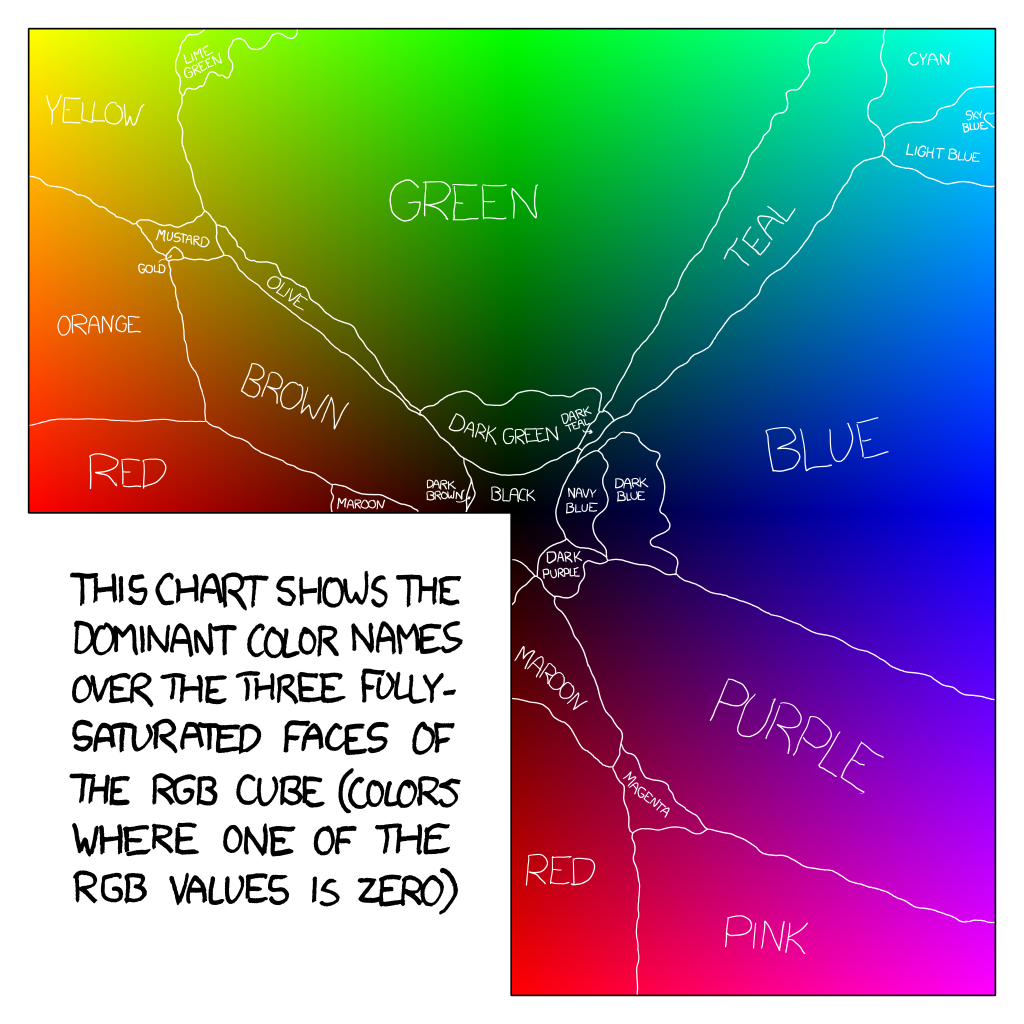
\includegraphics[width=0.5\textwidth]{images/satfaces_map.png}
  \caption[XKCD Color Survey: Color Dominant Names]{XKCD Color Survey: map of color dominant names.\protect\footnotemark{}}
  \label{fig:colornames_xkcd}
\end{figure}
%
Despite the fact XKCD's Color Survey was not a research realized with a scientific purpose, we decided to use it since it has plenty of information available to compare our results to, and it was executed with a great amount of users
which can verify it. We also found great compatibility between this survey and ours, since the values in the first were also presented in its maximum value of saturation (similar to our user study, in which we present colors in maximum hue).  \par
As said, these represent \gls{RGB} triplets but, being our user results all in accordance with the CIE XYZ Color Model, we needed some cleaning and processing to match the data our
responses. We \ul{converted the RGB to CIE XYZ values} and, then, \ul{divided all of the Color Bins in different tables}; there are 27 names atributted to colors, some have more triplets
(\emph{e.g.} blue, green or purple), but some have a smaller set, which could mean greater agreement to assign names to colors. These bins of color are represent with their frequencies, in table
\ref{table:colorbins}. \par
%
\begin{table}[htbp]
  \begin{center}
    \begin{tabular} {| c | c || c | c |}
      \hline
      Color Bin   &   Frequency   &   Color Bin   &   Frequency \\ \hline \hline
      Black       &   1782        &   Lime-Green  &   878 \\ \hline
      Blue        &   37725       &   Magenta     &   990 \\ \hline
      Brown       &   10499       &   Maroon      &   3283\\ \hline
      Cyan        &   2625        &   Mustard     &   711 \\ \hline
      Dark-Blue   &   2233        &   Navy-Blue   &   922 \\ \hline
      Dark-Brown  &   30          &   Olive       &   1336 \\ \hline
      Dark-Green  &   2927        &   Orange      &   9152 \\ \hline
      Dark-Purple &   669         &   Pink        &   12627 \\ \hline
      Dark-Red    &   2           &   Purple      &   25747 \\ \hline
      Dark-Teal   &   163         &   Red         &   15474 \\ \hline
      Gold        &   49          &   Sky-Blue    &   32 \\ \hline
      Green       &   47858       &   Teal        &   9007 \\ \hline
      Light-Blue  &   2078        &   Yellow      &   7808 \\ \hline
      Light-Green &   1           &   \-          &   \- \\
      \hline
    \end{tabular}
  \end{center}
  \caption[XKCD Color Survey: Color Bins]{XKCD Color Survey: color bins.}
  \label{table:colorbins}
\end{table}
%
The idea was to compare our answers with each color bin, to create a mapping between our users' values and commonly-used names; in order to simplify and speed up the computation
of the comparations, each color bin was drawn and the lowest polygon formed by the set of triplets of each bin was used to compare the values (instead of comparing each answer
with every triplet). Moreover, when processing these sets of RGB triplets, we left 3 color bins out of the game: \emph{Black} since it has no expressivity in the Chromaticity Diagram,
\emph{Dark-Red} and \emph{Light-Green} because they have very few triplets to be drawn. \par
%
\begin{figure}
  \centering
  \begin{minipage}{0.54\textwidth}
    \centering
    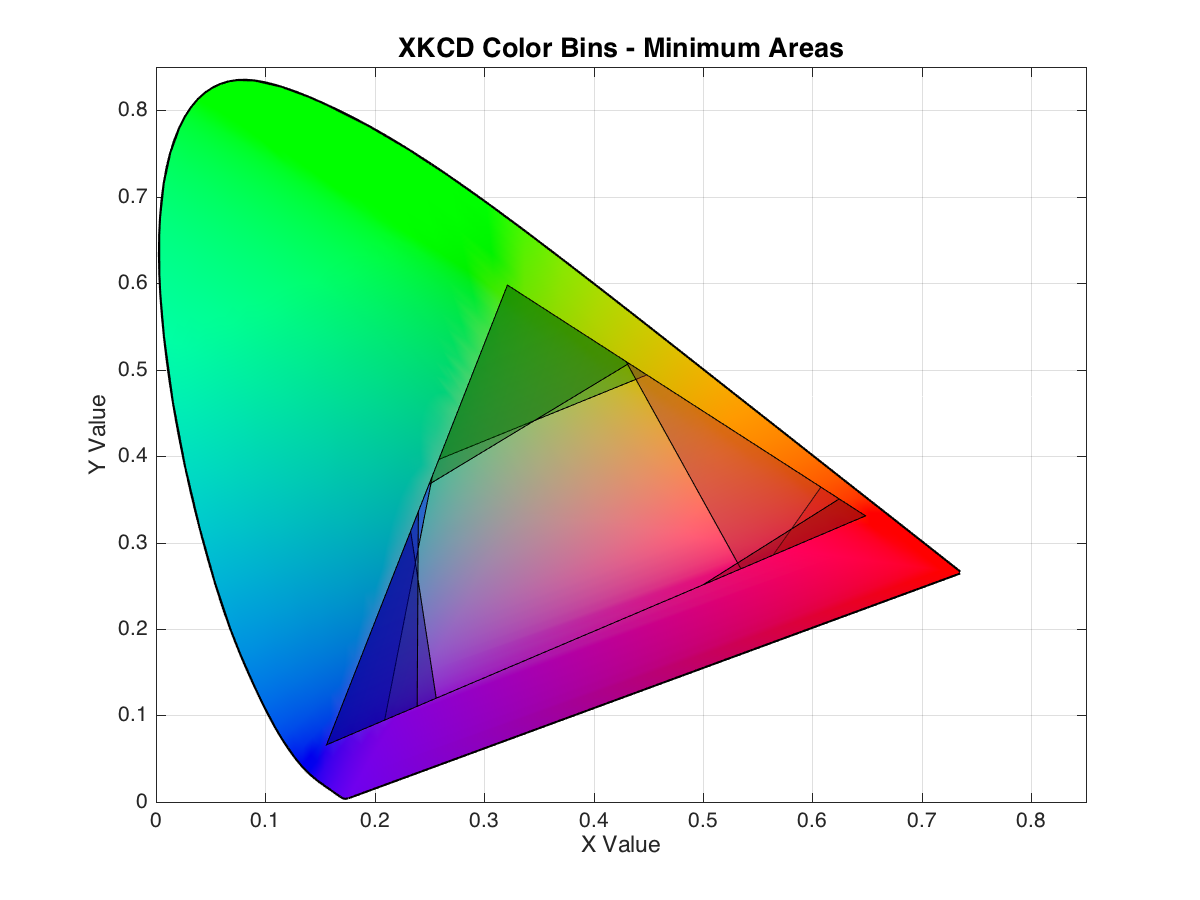
\includegraphics[width=0.9\textwidth]{images/colorbins_areas.png}
    \caption[XKCD Color Survey: Color Bins Minimum Areas]{XKCD Color Survey: Color Bins Minimum Areas.}
    \label{fig:colorbins_areas}
  \end{minipage}\hfill
  \begin{minipage}{0.45\textwidth}
    \centering
    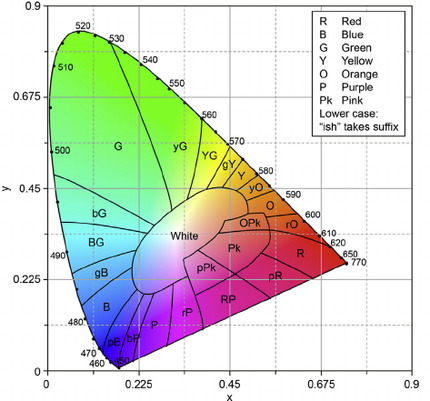
\includegraphics[width=0.87\textwidth]{images/cie_colors.png}
    \caption[Approximate Color Regions on CIE 1931 Chromaticity Diagram]{Approximate Color Regions on CIE 1931 Chromaticity Diagram. \cite{Fortner1997}}
    \label{fig:cie_colorregions}
  \end{minipage}
\end{figure}
%
However, we expected that when these color bins were drawn on a chromaticity diagram, they would create independent and more comprehensive shapes: we found that there are overlapping
values for some color bins (Figure \ref{fig:colorbins_areas}), which ultimately complicates the analysis because there is more than one possible name for the same color. For example, \emph{Blue} and \emph{Dark-Blue}
share 5 triplets: (0,0,76), (0,0,77), (0,0,78), (0,0,79) and (0,0,80); \emph{Green} and \emph{Dark-Green} share only 1 triplet, (0,57,0). No value was excluded from any color bin,
instead we solve the problem by allowing the program to find only one of the names and look no more after finding it. Moreover, the shapes created by each color bin can be depicted as \textbf{lines}
if they present contiguous values in the same edge of the triangle, or as \textbf{triangles} if the values are near the corner of the triangle and are distributed along two edges. The late situation is
represented in Figure \ref{fig:colorbins_triangle}\par
%
\begin{figure}
  \centering
  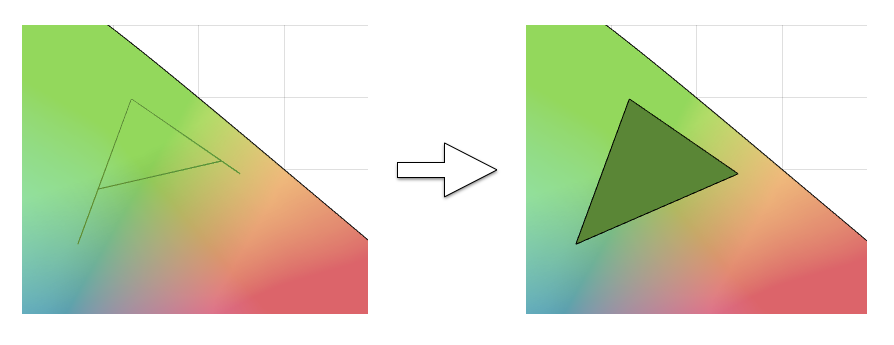
\includegraphics[width=0.8\textwidth]{images/colorbins_transformation.png}
  \caption[XKCD Color Survey: Color Bins Transformation]{XKCD Color Survey: Color Bins Transformation from line of points, to minimum polygon.}
  \label{fig:colornames_xkcd}
\end{figure} \par
%
Alternatively, we could have opted for another kind of color name detection, but its implementation would be out of the scope of this Master thesis and would take a much longer
analysis than the one performed. For instance, one could have gone for identifying the colors by analyzing their values and processing the wavelength originated, comparing the resulting
value with calculated areas, roughly defined by Brand Fortner \cite{Fortner1997} and represented on Figure \ref{fig:cie_colorregions}. This idea had one problem, which was the longevity
of its solution (dated from 1997), and the inexistence of a ready-to-go implementation, completed with an svg with all areas defined, had added weight on the decision. \par
%
Another possible method to decode color into name would be to interpret color values and associate a color temperature, being the late one compared against a well defined table
of values; the problem here was the non-existence of table of well defined values of color temperature. Further investigation is needed to ascertain the possibility of creating such
table. \par
%
\subsection{Outputs Generated}
\label{subsec:results_outputsgenerated}
%
Each script ends its execution when saving all the outputs contained in table \ref{table:outputs}: it generates a set of \gls{CSV} tables ready for being analyzed by
SPSS Program, besides creating a great amount of CIE chromaticity diagrams to support the analysis. As referred before, questions 18 to 32 do not generate any output about
white answers. \par
%
\begin{table}[htbp]
  \begin{center}
    \begin{tabular} {| c || c |}
      \hline
      Tables                    & Diagrams \\ \cline{1-2} \cline{1-2}
      age\_20\_results          & \multirow{3}{*}{\begin{tabular}[c]{@{}l@{}}For each Demographic Group:\\ - RGB, HSV and CMYK Responses \\ - CIE-L*C*h* and L*a*b* Responses \end{tabular}} \\ \cline{1-1}
      age\_20\_29\_results      &                 \\ \cline{1-1}
      age\_30\_39\_results      &                 \\ \cline{1-2}
      age\_40\_49\_results      & \multirow{4}{*}{\begin{tabular}[c]{@{}l@{}}For Laboratory Results:\\ - Regular and Daltonic Responses \\ - RGB, HSV and CMYK Responses \\ - CIE-L*C*h* and L*a*b* Responses \end{tabular}} \\ \cline{1-1}
      age\_50\_59\_results      &                 \\ \cline{1-1}
      age\_60\_results          &                 \\ \cline{1-1}
      gender\_female\_results   &                 \\ \cline{1-2}
      gender\_male\_results     & \multirow{5}{*}{\begin{tabular}[c]{@{}l@{}}For Online Results:\\ - Regular and Daltonic Responses \\ - Uncalibrated Responses \\ - RGB, HSV and CMYK Responses \\ - CIE-L*C*h* and L*a*b* Responses \end{tabular}} \\ \cline{1-1}
      gender\_other\_results    &                 \\ \cline{1-1}
      lab\_regular\_results     &                 \\ \cline{1-1}
      lab\_daltonic\_results    &                 \\ \cline{1-1}
      online\_regular\_results  &                 \\ \cline{1-2}
      online\_daltonic\_results & \multirow{3}{*}{\begin{tabular}[c]{@{}l@{}}For White Answers:\\ - White Responses \\ \end{tabular}} \\ \cline{1-1}
      online\_uncalibrated\_results &           \\ \cline{1-1}
      white\_answers            &               \\ \cline{1-2}
    \end{tabular}
  \end{center}
  \caption[Generated Outputs of Data Processing Phase]{Generated Outputs of Data Processing Phase.}
  \label{table:outputs}
\end{table}
%%%%%%%%%%%%%%%%%%%%%%%%%%%%%%%%%%%%%%%%%%%%%%%%%%%%%%%%%%%%%%%%%%%%%%%%%%%%%%%%%%%%%%%%%%%%%%%%%%%%%%%%%%%%%%%%%%%%%%%%%%%%%%%%%%%%%%%%%%%%%%%%%%%
%                                                                   RESULTS                                                                       %
%%%%%%%%%%%%%%%%%%%%%%%%%%%%%%%%%%%%%%%%%%%%%%%%%%%%%%%%%%%%%%%%%%%%%%%%%%%%%%%%%%%%%%%%%%%%%%%%%%%%%%%%%%%%%%%%%%%%%%%%%%%%%%%%%%%%%%%%%%%%%%%%%%%
\section{Results}
\label{sec:results_results}
%
In the following section, we perform a statistical analysis of the processed data obtained from the user study. The main data to be analyzed is the one obtained in the
laboratory environment, being the online data only the corroboration of the main data. We start by drawing a profile of users who responded the survey, characterizing them as the age,
country of residence, academic degree, along with other characteristics; after, we begin mapping answers to the questions raised in the beginning of study, also referred in section
\ref{sec:impl_objectives}, which comprises topics about \emph{Color Mixtures}, \emph{Color Models}, \emph{Color Naming} and consider differences between \emph{demographic groups}. \par
%
By the end of this chapter, we are going to discuss the results of the analysis and consider eventual implications for \gls{InfoVis} field of research. The following table \ref{table:summarize_results}
summarizes how the study is characterized: how many responses were given \emph{per} question, from which environment they came and the user sample from each demographic group. \par
%
\textbf{INCLUIR TABELA COM CONTAGEM.}
%
\subsection{User Profile}
\label{subsec:results_userprofile}
%
As previosuly said on section \ref{sec:results_datacleaning}, we gathered a total amount of 259 users with, at least, one valid answer: from the laboratory environment
we collected 28 users, and 231 from the online strand. All of these users gave valid answers along the Profiling, Calibration and Color Deficiencies Tests Phases: the information collected
in the Profiling page is the most important to compose a user profile. \par
Recalling section \ref{subsec:design_profiling}, we stablished that the most important informations to collect were the \emph{age}, the \emph{gender}, \emph{academic degree},
\emph{nationality} and \emph{country of residence}, as well as the \emph{native language} of each user. The table \ref{table:profiling_genderacademic} represents the frequencies of genders, ages and
academic degrees. \par
%
\begin{table}[htbp]
  \resizebox{\textwidth}{!} {
    \begin{tabular}{| l || c || c | c | c | c | c | c || c | c | c || c | c | c | c | c | c |}
      \hline
      \multicolumn{1}{|c||}{\multirow{2}{*}{Environment}} & \multirow{2}{*}{Users} & \multicolumn{6}{c||}{Ages}                                                           & \multicolumn{3}{c||}{Gender} & \multicolumn{6}{c|}{Academic Degree}                          \\ \cline{3-17}
      \multicolumn{1}{|c||}{}                             &                        & {[}0; 20{[} & {[}20; 29{]} & {[}30;39{]} & {[}40;49{]} & {[}50;59{]} & {[}60;90{]} & Female   & Male   & Other   & College & High-School & Bachelor & Master & Doctor & NoDegree \\ \hline
      Laboratory                                         & 28                     & 0           & 17           & 5           & 3           & 1           & 2            & 10       & 18     & 0        & 0       & 5           & 13       & 10     & 0      & 0        \\ \hline
      Online                                             & 231                    & 38          & 145          & 15          & 16          & 11          & 6            & 95       & 134    & 2        & 38      & 42          & 79       & 64     & 5      & 3        \\ \hline \hline
      Total                                              & 259                    & 38          & 162          & 20          & 19          & 12          & 8            & 105      & 152    & 2        & 38      & 47          & 92       & 74     & 5      & 3        \\ \hline
    \end{tabular}}
  \caption[Results: Profiling Information (Gender and Academic)]{Results: Profiling Information (Gender and Academic)}
  \label{table:profiling_genderacademic}
\end{table}
%
As seen above, our user sample is composed by 259 (100\%) users, being \textbf{105 (40.5\%) Females}, \textbf{152 (58.7\%) Males} and a minority of \textbf{2 (0.8\%) Other gendered users}: this sample age can
be characterized as being generally young ($\mu =$ 29.77, $\overline{X_{Age}} =$ 23, $\sigma =$ 40.30), surprinsigly having \textbf{8 users (3.09\%) aged above 60 years old} which could enhance some interesting
differences between age groups. Generally, our users have hight academic qualifications, representing \textbf{66.02\% of all users (Bachelor, Master and Doctoral Degrees)}, being \textbf{38 (14.67\%) users
qualified with College degree}, \textbf{47 (18.15\%) have a High-School degree} and only \textbf{3 (1.16\%) subjects do not presented any academic degree}. Between the laboratory and online environment, the distribution
of users remains with the same proportions: more male users than females, mostly aged between 20 and 29 years old (60.71\%) and the majority having a superior academic degree (46.43\% BSc and 35.71\% MSc). \par
%
\begin{table}[htbp]
  \resizebox{\textwidth}{!} {
  \begin{tabular}{| l || c || c | c | c | c | c | c || c | c | c | c | c | c || c | c | c |}
    \hline
    \multicolumn{1}{|c||}{\multirow{2}{*}{Environment}} & \multirow{2}{*}{Users} & \multicolumn{6}{c||}{Nacionality} & \multicolumn{6}{c||}{Country of Residence} & \multicolumn{3}{c|}{Languages} \\ \cline{3-17}
    \multicolumn{1}{|c||}{}                             &                        & CA  & ES & PT & UK & US & Others & CA   & DE   & GB   & PT   & US  & Others  & PT      & EN      & Others     \\ \hline
    Laboratory                                         & 28                     & 0   & 0  & 27 & 1  & 0  & 0      & 0    & 0    & 0    & 28   & 0   & 0       & 28      & 0       & 0          \\ \hline
    Online                                             & 231                    & 5   & 3  & 188& 6  & 11 & 18     & 5    & 3    & 9    & 189  & 11  & 14      & 188     & 29      & 14         \\ \hline \hline
    Total                                              & 259                    & 5   & 3  & 215& 7  & 11 & 18     & 5    & 3    & 9    & 217  & 11  & 14      & 216     & 29      & 14         \\ \hline
  \end{tabular}}
  \caption[Results: Profiling Information (Nationalities, Countries of Residence and Languages)]{Results: Profiling Information (Nationalities, Countries of Residence and Languages)}
  \label{table:profiling_nacionalities}
\end{table}
%
The table \ref{table:profiling_nacionalities} depicts nationalities, current countries of residence and native languages spoken by our users. From the 259 (100\%) participant users,
\textbf{215 (83.01\%) of them have Portuguese nationality}, \textbf{217 (83.78\%) live in Portugal} currently and \textbf{216 (83.40\%) speak Portuguese}; the second most influent group of users are from english-speaking
countries (United Kingdom, United States of America, and others). Other minor users which contributed to our survey came from Turkey, France, New Zealand, Sweden or even Antarctica (among others) -
\textbf{these countries represent only 5.41\%}. An ideal distribution of users would be such that it included enough users from all continents, which would give us room to investigate better the cultural
implications on the results; another interesting aspect would be to have the users of non-industrialized countries included in the sample, which was not accomplished in this study since an isolated vietnamese
user (0.39\% of the user sample) contributed to the study.
%
\subsection{Color Models}
\label{subsec:results_colormodels}
%
In this section, we will start by analyzing the results from each question, comparing the statistics collected from each color model. Then, we are going to decompose the results by color models and evaluate which questions
had the best and worst results. Along with the statistics we are going to present, in the end we are going to map them against the questions exposed before, clearly identifying them whenever they are answered. We would like
to emphasize that the important results are the ones collected in the laboratory environment: the online results will bridge and support the conclusions extracted from the laboratory conditions. The values presented as "distances"
are measured inside the finite interval between zero and one ($[0 ; 1]$), since the Chromaticity Diagram has its values comprised between this interval. \par
%
In order to improve this analysis, we present Table \ref{table:colormodels_distances_labonline} which contains the mean value for the distances to ideal color mixtures according to each color model: in green, it is marked the
best answer for each question, in each study environment (laboratory and online). \par
%
\begin{table}[!htbp]
  \resizebox{\textwidth}{!} {
  \begin{tabular}{@{}cccccccccccccc@{}}
                                  &                                                       & \multicolumn{2}{c}{Expected Colors}                         & \multicolumn{5}{c}{Laboratory Environment}                                                                                                                                                                                                                                      & \multicolumn{5}{c}{Online Environment}                                                                                                                                                                                                                                                                         \\ \cmidrule(l){3-14}
    \multirow{-2}{*}{Question ID} & \multirow{-2}{*}{Presented Color}                     & C1                           & \multicolumn{1}{c|}{C2}      & HSV                                                         & CIE-L*C*h*                                                 & CMYK                                                       & RGB                        & \multicolumn{1}{c||}{CIE-L*a*b*}                            & HSV                                                        & CIE-L*C*h*                                                 & CMYK                                                       & RGB                                                        & \multicolumn{1}{c|}{CIE-L*a*b*}                            \\ \midrule
    \multicolumn{1}{c}{1}       & \multicolumn{1}{c}{\cellcolor[HTML]{FFFF00}\#FFFF00} & \multicolumn{1}{c|}{Red}     & \multicolumn{1}{c|}{Green}   & \multicolumn{1}{c|}{0.13}                                   & \multicolumn{1}{c|}{0.2}                                   & \multicolumn{1}{c|}{\cellcolor[HTML]{32CB00}\textbf{0.09}} & \multicolumn{1}{c|}{0.12}  & \multicolumn{1}{c||}{0.12}                                  & \multicolumn{1}{c|}{0.07}                                  & \multicolumn{1}{c|}{0.21}                                  & \multicolumn{1}{c|}{\cellcolor[HTML]{32CB00}\textbf{0.06}} & \multicolumn{1}{c|}{0.07}                                  & \multicolumn{1}{c|}{0.07}                                  \\ \midrule
    \multicolumn{1}{c}{2}       & \multicolumn{1}{c}{\cellcolor[HTML]{FF00FF}\#FF00FF} & \multicolumn{1}{c|}{Red}     & \multicolumn{1}{c|}{Blue}    & \multicolumn{1}{c|}{0.22}                                   & \multicolumn{1}{c|}{0.16}                                  & \multicolumn{1}{c|}{\cellcolor[HTML]{32CB00}\textbf{0.11}} & \multicolumn{1}{c|}{0.17}  & \multicolumn{1}{c||}{0.16}                                  & \multicolumn{1}{c|}{0.15}                                  & \multicolumn{1}{c|}{0.16}                                  & \multicolumn{1}{c|}{\cellcolor[HTML]{32CB00}\textbf{0.08}} & \multicolumn{1}{c|}{0.1}                                   & \multicolumn{1}{c|}{0.12}                                  \\ \midrule
    \multicolumn{1}{c}{3}       & \multicolumn{1}{c}{\cellcolor[HTML]{80FF00}\#80FF00} & \multicolumn{1}{c|}{Red}     & \multicolumn{1}{c|}{Cyan}    & \multicolumn{1}{c|}{\cellcolor[HTML]{32CB00}\textbf{0.045}} & \multicolumn{1}{c|}{0.215}                                 & \multicolumn{1}{c|}{0.05}                                  & \multicolumn{1}{c|}{0.095} & \multicolumn{1}{c||}{0.11}                                  & \multicolumn{1}{c|}{\cellcolor[HTML]{32CB00}\textbf{0.04}} & \multicolumn{1}{c|}{0.21}                                  & \multicolumn{1}{c|}{0.06}                                  & \multicolumn{1}{c|}{0.11}                                  & \multicolumn{1}{c|}{0.11}                                  \\ \midrule
    \multicolumn{1}{c}{4}       & \multicolumn{1}{c}{\cellcolor[HTML]{7F00FF}\#7F00FF} & \multicolumn{1}{c|}{Red}     & \multicolumn{1}{c|}{Cyan}    & \multicolumn{1}{c|}{0.12}                                   & \multicolumn{4}{c||}{}                                                                                                                                                                                             & \multicolumn{1}{c|}{0.11}                                  & \multicolumn{4}{c|}{}                                                                                                                                                                                                                             \\ \midrule
    \multicolumn{1}{c}{5}       & \multicolumn{1}{c}{\cellcolor[HTML]{FF0080}\#FF0080} & \multicolumn{1}{c|}{Red}     & \multicolumn{1}{c|}{Magenta} & \multicolumn{1}{c|}{0.17}                                   & \multicolumn{1}{c|}{0.15}                                  & \multicolumn{1}{c|}{\cellcolor[HTML]{32CB00}\textbf{0.13}} & \multicolumn{1}{c|}{0.14}  & \multicolumn{1}{c||}{0.14}                                  & \multicolumn{1}{c|}{0.16}                                  & \multicolumn{1}{c|}{0.15}                                  & \multicolumn{1}{c|}{\cellcolor[HTML]{32CB00}\textbf{0.13}} & \multicolumn{1}{c|}{0.14}                                  & \multicolumn{1}{c|}{0.11}                                  \\ \midrule
    \multicolumn{1}{c}{6}       & \multicolumn{1}{c}{\cellcolor[HTML]{FF8000}\#FF8000} & \multicolumn{1}{c|}{Red}     & \multicolumn{1}{c|}{Yellow}  & \multicolumn{1}{c|}{0.07}                                   & \multicolumn{1}{c|}{0.13}                                  & \multicolumn{1}{c|}{0.06}                                  & \multicolumn{1}{c|}{0.08}  & \multicolumn{1}{c||}{\cellcolor[HTML]{32CB00}\textbf{0.05}} & \multicolumn{1}{c|}{0.03}                                  & \multicolumn{1}{c|}{0.14}                                  & \multicolumn{1}{c|}{0.03}                                  & \multicolumn{1}{c|}{0.04}                                  & \multicolumn{1}{c|}{\cellcolor[HTML]{32CB00}\textbf{0.02}} \\ \midrule
    \multicolumn{1}{c}{7}       & \multicolumn{1}{c}{\cellcolor[HTML]{0000FF}\#0000FF} & \multicolumn{1}{c|}{Cyan}    & \multicolumn{1}{c|}{Magenta} & \multicolumn{1}{c|}{0.16}                                   & \multicolumn{1}{c|}{0.23}                                  & \multicolumn{1}{c|}{\cellcolor[HTML]{32CB00}\textbf{0.10}} & \multicolumn{1}{c|}{0.15}  & \multicolumn{1}{c||}{0.17}                                  & \multicolumn{1}{c|}{0.13}                                  & \multicolumn{1}{c|}{0.18}                                  & \multicolumn{1}{c|}{\cellcolor[HTML]{32CB00}\textbf{0.11}} & \multicolumn{1}{c|}{0.17}                                  & \multicolumn{1}{c|}{0.22}                                  \\ \midrule
    \multicolumn{1}{c}{8}       & \multicolumn{1}{c}{\cellcolor[HTML]{FF0000}\#FF0000} & \multicolumn{1}{c|}{Magenta} & \multicolumn{1}{c|}{Yellow}  & \multicolumn{1}{c|}{\cellcolor[HTML]{32CB00}\textbf{0.10}}  & \multicolumn{1}{c|}{0.17}                                  & \multicolumn{1}{c|}{\cellcolor[HTML]{32CB00}\textbf{0.10}} & \multicolumn{1}{c|}{0.13}  & \multicolumn{1}{c||}{0.13}                                  & \multicolumn{1}{c|}{0.10}                                  & \multicolumn{1}{c|}{\cellcolor[HTML]{32CB00}\textbf{0.09}} & \multicolumn{1}{c|}{0.12}                                  & \multicolumn{1}{c|}{0.14}                                  & \multicolumn{1}{c|}{0.16}                                  \\ \midrule
    \multicolumn{1}{c}{9}       & \multicolumn{1}{c}{\cellcolor[HTML]{00FF80}\#00FF80} & \multicolumn{1}{c|}{Green}   & \multicolumn{1}{c|}{Cyan}    & \multicolumn{1}{c|}{0.13}                                   & \multicolumn{1}{c|}{0.16}                                  & \multicolumn{1}{c|}{\cellcolor[HTML]{32CB00}\textbf{0.09}} & \multicolumn{1}{c|}{0.10}  & \multicolumn{1}{c||}{0.11}                                  & \multicolumn{1}{c|}{0.11}                                  & \multicolumn{1}{c|}{0.13}                                  & \multicolumn{1}{c|}{\cellcolor[HTML]{32CB00}\textbf{0.10}} & \multicolumn{1}{c|}{\cellcolor[HTML]{32CB00}\textbf{0.10}} & \multicolumn{1}{c|}{0.11}                                  \\ \midrule
    \multicolumn{1}{c}{10}      & \multicolumn{1}{c}{\cellcolor[HTML]{0080FF}\#0080FF} & \multicolumn{1}{c|}{Green}   & \multicolumn{1}{c|}{Magenta} & \multicolumn{1}{c|}{0.30}                                   & \multicolumn{1}{c|}{0.26}                                  & \multicolumn{1}{c|}{\cellcolor[HTML]{32CB00}\textbf{0.13}} & \multicolumn{1}{c|}{0.21}  & \multicolumn{1}{c||}{0.20}                                  & \multicolumn{1}{c|}{0.17}                                  & \multicolumn{1}{c|}{0.27}                                  & \multicolumn{1}{c|}{\cellcolor[HTML]{32CB00}\textbf{0.13}} & \multicolumn{1}{c|}{0.20}                                  & \multicolumn{1}{c|}{0.22}                                  \\ \midrule
    \multicolumn{1}{c}{11}      & \multicolumn{1}{c}{\cellcolor[HTML]{FF8000}\#FF8000} & \multicolumn{1}{c|}{Green}   & \multicolumn{1}{c|}{Magenta} & \multicolumn{1}{c|}{\cellcolor[HTML]{32CB00}\textbf{0.06}}  & \multicolumn{4}{c||}{}                                                                                                                                                                                             & \multicolumn{1}{c|}{\cellcolor[HTML]{32CB00}\textbf{0.04}} & \multicolumn{4}{c|}{}                                                                                                                                                                                                                             \\ \midrule
    \multicolumn{1}{c}{12}      & \multicolumn{1}{c}{\cellcolor[HTML]{80FF00}\#80FF00} & \multicolumn{1}{c|}{Green}   & \multicolumn{1}{c|}{Yellow}  & \multicolumn{1}{c|}{\cellcolor[HTML]{32CB00}\textbf{0.11}}  & \multicolumn{1}{c|}{0.23}                                  & \multicolumn{1}{c|}{0.13}                                  & \multicolumn{1}{c|}{0.15}  & \multicolumn{1}{c||}{0.17}                                  & \multicolumn{1}{c|}{\cellcolor[HTML]{32CB00}\textbf{0.08}} & \multicolumn{1}{c|}{0.24}                                  & \multicolumn{1}{c|}{0.12}                                  & \multicolumn{1}{c|}{0.13}                                  & \multicolumn{1}{c|}{0.15}                                  \\ \midrule
    \multicolumn{1}{c}{13}      & \multicolumn{1}{c}{\cellcolor[HTML]{0080FF}\#0080FF} & \multicolumn{1}{c|}{Blue}    & \multicolumn{1}{c|}{Cyan}    & \multicolumn{1}{c|}{0.27}                                   & \multicolumn{1}{c|}{\cellcolor[HTML]{32CB00}\textbf{0.17}} & \multicolumn{1}{c|}{0.19}                                  & \multicolumn{1}{c|}{0.25}  & \multicolumn{1}{c||}{0.23}                                  & \multicolumn{1}{c|}{0.14}                                  & \multicolumn{1}{c|}{0.20}                                  & \multicolumn{1}{c|}{0.14}                                  & \multicolumn{1}{c|}{\cellcolor[HTML]{32CB00}\textbf{0.13}} & \multicolumn{1}{c|}{0.14}                                  \\ \midrule
    \multicolumn{1}{c}{14}      & \multicolumn{1}{c}{\cellcolor[HTML]{8000FF}\#8000FF} & \multicolumn{1}{c|}{Blue}    & \multicolumn{1}{c|}{Magenta} & \multicolumn{1}{c|}{0.12}                                   & \multicolumn{1}{c|}{0.30}                                  & \multicolumn{1}{c|}{\cellcolor[HTML]{32CB00}\textbf{0.10}} & \multicolumn{1}{c|}{0.13}  & \multicolumn{1}{c||}{0.13}                                  & \multicolumn{1}{c|}{0.10}                                  & \multicolumn{1}{c|}{0.29}                                  & \multicolumn{1}{c|}{\cellcolor[HTML]{32CB00}\textbf{0.09}} & \multicolumn{1}{c|}{0.11}                                  & \multicolumn{1}{c|}{0.12}                                  \\ \midrule
    \multicolumn{1}{c}{15}      & \multicolumn{1}{c}{\cellcolor[HTML]{00FF80}\#00FF80} & \multicolumn{1}{c|}{Blue}    & \multicolumn{1}{c|}{Yellow}  & \multicolumn{1}{c|}{0.09}                                   & \multicolumn{1}{c|}{0.30}                                  & \multicolumn{1}{c|}{\cellcolor[HTML]{32CB00}\textbf{0.06}} & \multicolumn{1}{c|}{0.11}  & \multicolumn{1}{c||}{0.13}                                  & \multicolumn{1}{c|}{0.11}                                  & \multicolumn{1}{c|}{0.30}                                  & \multicolumn{1}{c|}{\cellcolor[HTML]{32CB00}\textbf{0.06}} & \multicolumn{1}{c|}{0.11}                                  & \multicolumn{1}{c|}{0.13}                                  \\ \midrule
    \multicolumn{1}{c}{16}      & \multicolumn{1}{c}{\cellcolor[HTML]{FF007F}\#FF007F} & \multicolumn{1}{c|}{Blue}    & \multicolumn{1}{c|}{Yellow}  & \multicolumn{1}{c|}{0.21}                                   & \multicolumn{4}{c||}{}                                                                                                                                                                                             & \multicolumn{1}{c|}{0.19}                                  & \multicolumn{4}{c|}{}                                                                                                                                                                                                                             \\ \midrule
    \multicolumn{1}{c}{17}      & \multicolumn{1}{c}{\cellcolor[HTML]{00FF00}\#00FF00} & \multicolumn{1}{c|}{Cyan}    & \multicolumn{1}{c|}{Yellow}  & \multicolumn{1}{c|}{0.07}                                   & \multicolumn{1}{c|}{0.16}                                  & \multicolumn{1}{c|}{\cellcolor[HTML]{32CB00}\textbf{0.05}} & \multicolumn{1}{c|}{0.10}  & \multicolumn{1}{c||}{0.11}                                  & \multicolumn{1}{c|}{0.08}                                  & \multicolumn{1}{c|}{0.17}                                  & \multicolumn{1}{c|}{\cellcolor[HTML]{32CB00}\textbf{0.05}} & \multicolumn{1}{c|}{0.10}                                  & \multicolumn{1}{c|}{0.11}                                  \\ \bottomrule
  \end{tabular}}
  \caption[Results: Distances of Results Mixed in each Color Model]{Results: Distances of Results Mixed in each Color Model, for each question, with the distance from itself to the ideal pre-calculated answer. Colored
  in green are, the color model which has the best result, \emph{per} question, in each environment.}
  \label{table:colormodels_distances_labonline}
\end{table}
%
As referred before, each answer pair given from our users on questions 1 to 17 (one color given, two colors asked) was blendend in 5 color models: HSV, CIE-L*C*h*, CMYK, RGB and CIE-L*a*b*. Then, the XY coordinates of each resulting
mixture were mapped on a CIE Chromaticity Diagram, the centroids of each group of mixtures was calculated, and the distance from each centroid to the (ideal) pre-calculated answer was measured. The table \ref{table:colormodels_distances_labonline}
represents the distance measured associated to each color model, for every laboratory result. \par
%
%%%%%%%%%%%%%%%%%%%%%%%%%%%%%%%%%%%%%%%%%%%%%%%%%%%%%%%%%%%%%%%%%%%%%%%%%%%%%%%%%
%
\subsubsection{Analyzing Questions}
\label{subsubsec:questions_analyzing}
%
The importance of breaking down the evaluation into questions is such that, it is relevant to understand, at least, which color models have the best results for each mixture. The results from this section will be critical
to determine later which color models are more compatible with each mixture, which model yields better results and others who do not. A crucial reminder is that each question set for this user study is blended in HSV Color
Model: the primitives anticipated for the blends are, then, colors required to produce the result according to the HSV Color Model. The triples presented in each shaded cell of tables below, are XYZ coordinates for the CIE
XYZ Color Model. \par
%
\paragraph{\ul{Question One}}
%
This is the only question in the entire study which has \ul{yellow as the resulting color of the blending}. The expected colors are \ul{Red and Green}, two primitives from RGB Color Model. Table \ref{table:lab_q1_expected} shows the
expected colors when mixing in each color model: HSV, CIE-L*C*h*, CMYK, RGB and CIE-L*a*b*. \par
%
As said before, each answer-pair was blended according to those 5 models; after processing data from each question, we performed the mean calculation over the entire set of distances, between each resulting blend and the ideal blend (according
to every color model). This produced the results reported on Table \ref{table:lab_q1_expected}. \par
%
One can observe that the model which presents the lowest mean value is the CMYK ($\tilde{x} = 0.09$), possibily indicating that this model yields the best results for this question, while HSV, RGB and CIE-L*a*b* have closer values.
A Friedman Test showed that there are, indeed, significant differences ($\chi^2 = 48.568$, $p < 0.05$) between each color model. \par
%
Further analyis with the Wilcoxon Test reveals that CMYK ($p < 0.05$) has, in fact, very different responses from the other color models, which leads us to conclude that \textbf{the CMYK Color Model is the best model to represent yellow blends}.
Since HSV, RGB and CIE-L*a*b* have similar mean values, we tried to compare them between each other: \textbf{there is no statiscally significant differences among HSV, RGB and CIE-L*a*b*, whereby there is insufficient information to evaluate this
color models regarding this color mixture}. According to table, it is also possible to say that \textbf{CMYK Color Model presents a low deviation}, not only in laboratory results ($\sigma_{lab} = 0.06$), but
such value is corroborated by the online users ($\sigma_{online} = 0.06$). \par
%
It is safe to say that \textbf{CIE-L*C*h* has the worst performance against the other color models}, since its mean is the highest of all ($\tilde{x} = 0.20$), and the values from Wilcoxon Test ($p < 0.005$) indicates that this color model has
statistically signifcant differences every other model. \textbf{This results are corroborated by the online users}.
%
\begin{table}[H]
  \resizebox{\textwidth}{!} {
  \begin{tabular}{lccccccccccccc}
    \hline
    \multicolumn{1}{c}{}                              &                                      & \multicolumn{2}{c}{Expected Colors}                   & \multicolumn{10}{c}{Possible Results}                                                                                                                                                                                                                                                                                        \\ \cline{3-14}
    \multicolumn{1}{c}{\multirow{-2}{*}{Question ID}} & \multirow{-2}{*}{Given Color}        & C1                       & C2                         & \multicolumn{2}{c}{HSV}                                        & \multicolumn{2}{c}{CIE-L*C*h*}                                 & \multicolumn{2}{c}{CMYK}                                       & \multicolumn{2}{c}{RGB}                                        & \multicolumn{2}{c}{CIE-L*a*b*}                                 \\ \hline
    \multicolumn{1}{c}{1}                             & \cellcolor[HTML]{FFFF00}(77, 93, 14) & \multicolumn{1}{c|}{Red} & \multicolumn{1}{c|}{Green} & \multicolumn{2}{c|}{\cellcolor[HTML]{FFFF00}(77, 93, 14)}      & \multicolumn{2}{c|}{\cellcolor[HTML]{D7A700}(42, 42, 6)}       & \multicolumn{2}{c|}{\cellcolor[HTML]{808000}(17, 20, 3)}       & \multicolumn{2}{c|}{\cellcolor[HTML]{808000}(17, 20, 3)}       & \multicolumn{2}{c|}{\cellcolor[HTML]{C9AB00}(39, 42, 6)}       \\ \hline
                                                      & \multicolumn{1}{l}{}                 & \multicolumn{1}{l}{}     & \multicolumn{1}{l}{}       & \multicolumn{1}{c}{$\tilde{x}$} & \multicolumn{1}{c}{$\sigma$} & \multicolumn{1}{c}{$\tilde{x}$} & \multicolumn{1}{c}{$\sigma$} & \multicolumn{1}{c}{$\tilde{x}$} & \multicolumn{1}{c}{$\sigma$} & \multicolumn{1}{c}{$\tilde{x}$} & \multicolumn{1}{c}{$\sigma$} & \multicolumn{1}{c}{$\tilde{x}$} & \multicolumn{1}{c}{$\sigma$} \\ \hline
    \multicolumn{4}{l}{Distance to Objective - Laboratory}                                                                                           & \multicolumn{1}{|c}{0.13}       & \multicolumn{1}{c|}{0.08}    & \multicolumn{1}{|c}{0.2}        & \multicolumn{1}{c|}{0.06}    & \multicolumn{1}{|c}{\textbf{0.09}}       & \multicolumn{1}{c|}{0.06}    & \multicolumn{1}{|c}{0.12}       & \multicolumn{1}{c|}{0.08}    & \multicolumn{1}{|c}{0.12}       & \multicolumn{1}{c|}{0.08}    \\
    \multicolumn{4}{l}{Distance to Objective - Online}                                                                                               & \multicolumn{1}{|c}{0.07}       & \multicolumn{1}{c|}{0.09}    & \multicolumn{1}{|c}{0.21}       & \multicolumn{1}{c|}{0.07}    & \multicolumn{1}{|c}{\textbf{0.06}}       & \multicolumn{1}{c|}{0.06}    & \multicolumn{1}{|c}{0.07}       & \multicolumn{1}{c|}{0.09}    & \multicolumn{1}{|c}{0.07}       & \multicolumn{1}{c|}{0.08}    \\ \hline
    \end{tabular}}
  \caption[Question 1, with expected Results.]{Question 1, with expected colors, possible results, mean and standard deviation of distances to Objective colors.}
  \label{table:lab_q1_expected}
\end{table}
%
\paragraph{\ul{Question Two}}
%
This question \ul{presents a Magenta color} and expects to receive, from the user, the \ul{Red and Blue colors} according to the HSV Color Model. \par
%
The colors were blended, and again the mean values over distances were calculated, as Table \ref{table:lab_q2_expected} shows. It is observable that CMYK Color Model presents, yet again,
the lowest mean value for distance to ideal answer ($\tilde{x} = 0.11$), whilst its standard deviation is also the lowest between both study environments. \par
%
However, it is not safe to say that which color model had the worst results: judging by laboratory values, the HSV Color Model would not only the have highest mean distance, but also
the largest deviation of answers; yet, evaluating the online results, it would CIE-L*C*h* to occupy such position. Performing a Friedman Test, we can conclude that there are, in fact,
significant differences ($\chi^2 = 22.041$, $p < 0.05$) between the color models; post hoc Wilcoxon Analysis ($p < 0.05$) reveals CMYK has statistically different results from every other
color model, therefore concluding that \textbf{CMYK has the best solution for this blending}, according to users' responses. \par
%
The tendency of results to blend Magenta in CMYK Color Model, could be explained by the fact that magenta is a primitive color of such model, therefore leading the user to blend it
accordingly. \par
%
In this question, \textbf{CIE-L*C*h* has only significant differences with HSV ($p < 0.05$)}, which is far opposite from question 1. The online results for this question validate the
laboratory experience.
%
\begin{table}[H]
  \resizebox{\textwidth}{!} {
  \begin{tabular}{lccccccccccccc}
    \hline
    \multicolumn{1}{c}{}                              &                                      & \multicolumn{2}{c}{Expected Colors}                   & \multicolumn{10}{c}{Possible Results}                                                                                                                                                                                                                                                                                        \\ \cline{3-14}
    \multicolumn{1}{c}{\multirow{-2}{*}{Question ID}} & \multirow{-2}{*}{Given Color}        & C1                       & C2                         & \multicolumn{2}{c}{HSV}                                        & \multicolumn{2}{c}{CIE-L*C*h*}                                 & \multicolumn{2}{c}{CMYK}                                       & \multicolumn{2}{c}{RGB}                                        & \multicolumn{2}{c}{CIE-L*a*b*}                                 \\ \hline
    \multicolumn{1}{c}{2}                             & \cellcolor[HTML]{FF00FF}(59, 28, 97) & \multicolumn{1}{c|}{Red} & \multicolumn{1}{c|}{Blue}  & \multicolumn{2}{c|}{\cellcolor[HTML]{FF00FF}(59, 28, 97)}      & \multicolumn{2}{c|}{\cellcolor[HTML]{FB0080}(44, 22, 22)}       & \multicolumn{2}{c|}{\cellcolor[HTML]{800080}(13, 6, 21)}       & \multicolumn{2}{c|}{\cellcolor[HTML]{800080}(13, 6, 21)}       & \multicolumn{2}{c|}{\cellcolor[HTML]{CA0088}(29, 14, 25)}       \\ \hline
                                                      & \multicolumn{1}{l}{}                 & \multicolumn{1}{l}{}     & \multicolumn{1}{l}{}       & \multicolumn{1}{c}{$\tilde{x}$} & \multicolumn{1}{c}{$\sigma$} & \multicolumn{1}{c}{$\tilde{x}$} & \multicolumn{1}{c}{$\sigma$} & \multicolumn{1}{c}{$\tilde{x}$} & \multicolumn{1}{c}{$\sigma$} & \multicolumn{1}{c}{$\tilde{x}$} & \multicolumn{1}{c}{$\sigma$} & \multicolumn{1}{c}{$\tilde{x}$} & \multicolumn{1}{c}{$\sigma$} \\ \hline
    \multicolumn{4}{l}{Distance to Objective - Laboratory}                                                                                           & \multicolumn{1}{|c}{0.22}       & \multicolumn{1}{c|}{0.13}    & \multicolumn{1}{|c}{0.16}       & \multicolumn{1}{c|}{0.09}    & \multicolumn{1}{|c}{\textbf{0.11}}       & \multicolumn{1}{c|}{0.06}    & \multicolumn{1}{|c}{0.17}       & \multicolumn{1}{c|}{0.11}    & \multicolumn{1}{|c}{0.16}       & \multicolumn{1}{c|}{0.08}    \\
    \multicolumn{4}{l}{Distance to Objective - Online}                                                                                               & \multicolumn{1}{|c}{0.15}       & \multicolumn{1}{c|}{0.13}    & \multicolumn{1}{|c}{0.16}       & \multicolumn{1}{c|}{0.08}    & \multicolumn{1}{|c}{\textbf{0.08}}       & \multicolumn{1}{c|}{0.04}    & \multicolumn{1}{|c}{0.1}        & \multicolumn{1}{c|}{0.08}    & \multicolumn{1}{|c}{0.12}       & \multicolumn{1}{c|}{0.05}    \\ \hline
    \end{tabular}}
  \caption[Question 2, with expected Results.]{Question 2, with expected colors, possible results, mean and standard deviation of distances to Objective colors.}
  \label{table:lab_q2_expected}
\end{table}
%
%
\paragraph{\ul{Question Three}}
%
This question \ul{presents a Green color} and expects to receive, from the user, the \ul{Red and Cyan colors}. According to the HSV Color Model, Red and Cyan are positioned in
opposite angles in the Hue Circle of Colors: therefore, blending these opposite colors that output two different colors. It is important to study to which color the users tend
to blend; this question should be evaluate along with Question Four, which has the contrary output. \par
%
The colors were blended, and again the mean values over distances were calculated, as Table \ref{table:lab_q3_expected} shows. It is observable that CMYK Color Model presents
the lowest mean value for distance to ideal answer ($\tilde{x} = 0.05$); however, the standard deviation for the HSV Color Model is the highest between both study environments ($\sigma = 0.12$). \par
%
Running the Friedman Test, we can conclude that there are significant differences ($\chi^2 = 84.448$, $p < 0.05$) between the color models; Wilcoxon Analysis ($p < 0.05$) reveals
CMYK has statistically different results from other color models (except RGB), therefore concluding that \textbf{CMYK has the best solution for this blending}, according to
users' responses. CIE-L*C*h* is again the lower color model being significantly different from every other color model. The second best color model is \textbf{CMYK}, with
statistically different results with every color model, except for \textbf{HSV}. \par
%
Once again, these results are validated by the online users' dataset. The results from this question will be useful later, when analyzing question twelve.
%
\begin{table}[H]
  \resizebox{\textwidth}{!} {
  \begin{tabular}{lccccccccccccc}
    \hline
    \multicolumn{1}{c}{}                              &                                      & \multicolumn{2}{c}{Expected Colors}                   & \multicolumn{10}{c}{Possible Results}                                                                                                                                                                                                                                                                                        \\ \cline{3-14}
    \multicolumn{1}{c}{\multirow{-2}{*}{Question ID}} & \multirow{-2}{*}{Given Color}        & C1                       & C2                         & \multicolumn{2}{c}{HSV}                                        & \multicolumn{2}{c}{CIE-L*C*h*}                                 & \multicolumn{2}{c}{CMYK}                                       & \multicolumn{2}{c}{RGB}                                        & \multicolumn{2}{c}{CIE-L*a*b*}                                 \\ \hline
    \multicolumn{1}{c}{3}                             & \cellcolor[HTML]{80FF00}(45, 76, 12) & \multicolumn{1}{c|}{Red} & \multicolumn{1}{c|}{Cyan}  & \multicolumn{2}{c|}{\cellcolor[HTML]{80FF00}(45, 76, 12)}      & \multicolumn{2}{c|}{\cellcolor[HTML]{91C01D}(31, 44, 8)}       & \multicolumn{2}{c|}{\cellcolor[HTML]{808080}(21, 22, 24)}       & \multicolumn{2}{c|}{\cellcolor[HTML]{808080}(21, 22, 24)}       & \multicolumn{2}{c|}{\cellcolor[HTML]{DDA581}(47, 44, 27)}       \\ \hline
                                                      & \multicolumn{1}{l}{}                 & \multicolumn{1}{l}{}     & \multicolumn{1}{l}{}       & \multicolumn{1}{c}{$\tilde{x}$} & \multicolumn{1}{c}{$\sigma$} & \multicolumn{1}{c}{$\tilde{x}$} & \multicolumn{1}{c}{$\sigma$} & \multicolumn{1}{c}{$\tilde{x}$} & \multicolumn{1}{c}{$\sigma$} & \multicolumn{1}{c}{$\tilde{x}$} & \multicolumn{1}{c}{$\sigma$} & \multicolumn{1}{c}{$\tilde{x}$} & \multicolumn{1}{c}{$\sigma$} \\ \hline
    \multicolumn{4}{l}{Distance to Objective - Laboratory}                                                                                           & \multicolumn{1}{|c}{0.094}       & \multicolumn{1}{c|}{0.12}    & \multicolumn{1}{|c}{0.23}       & \multicolumn{1}{c|}{0.06}    & \multicolumn{1}{|c}{\textbf{0.061}}       & \multicolumn{1}{c|}{0.03}    & \multicolumn{1}{|c}{0.11}       & \multicolumn{1}{c|}{0.06}    & \multicolumn{1}{|c}{0.12}       & \multicolumn{1}{c|}{0.04}    \\
    \multicolumn{4}{l}{Distance to Objective - Online}                                                                                               & \multicolumn{1}{|c}{\textbf{0.07}}        & \multicolumn{1}{c|}{0.09}    & \multicolumn{1}{|c}{0.23}        & \multicolumn{1}{c|}{0.06}    & \multicolumn{1}{|c}{\textbf{0.07}}       & \multicolumn{1}{c|}{0.03}    & \multicolumn{1}{|c}{0.12}        & \multicolumn{1}{c|}{0.06}    & \multicolumn{1}{|c}{0.13}       & \multicolumn{1}{c|}{0.04}    \\ \hline
    \end{tabular}}
  \caption[Question 3, with expected Results.]{Question 3, with expected colors, possible results, mean and standard deviation of distances to Objective colors.}
  \label{table:lab_q3_expected}
\end{table}
%
\paragraph{\ul{Question Four}}
%
As explained in previous question, this one is the second possible output from the blend of \ul{Red and Cyan colors}. This color has no matching color pairs in the other models,
since this color is only obtained in the HSV Color Model. Comparing the results for the HSV Color Model of both questions, mean distances are quite lower for question thirteen
($\tilde{x} = 0.045$), whilst the deviation of answers is higher in both questions. \par
%
Based on these results, corroborated by the online users, we can conclude \textbf{users tend to blend in CMYK Color Model to obtain a green color}, \textbf{mixing red and cyan
does not generate a purple shade, according to users' expectations}. The results from this question can be found in table \ref{table:lab_q4_expected}.
%
\begin{table}[H]
  \resizebox{\textwidth}{!} {
  \begin{tabular}{lccccccccccccc}
    \hline
    \multicolumn{1}{c}{}                              &                                      & \multicolumn{2}{c}{Expected Colors}                   & \multicolumn{10}{c}{Possible Results}                                                                                                                                                                                                                                                                                        \\ \cline{3-14}
    \multicolumn{1}{c}{\multirow{-2}{*}{Question ID}} & \multirow{-2}{*}{Given Color}        & C1                       & C2                         & \multicolumn{2}{c}{HSV}                                        & \multicolumn{2}{c}{CIE-L*C*h*}                                 & \multicolumn{2}{c}{CMYK}                                       & \multicolumn{2}{c}{RGB}                                        & \multicolumn{2}{c}{CIE-L*a*b*}                                 \\ \hline
    \multicolumn{1}{c}{4}                             & \cellcolor[HTML]{7F00FF}(27, 12, 95) & \multicolumn{1}{c|}{Red} & \multicolumn{1}{c|}{Cyan}  & \multicolumn{2}{c|}{\cellcolor[HTML]{FF00FF}(59, 28, 97)}      & \multicolumn{2}{c|}{-}       & \multicolumn{2}{c|}{-}        & \multicolumn{2}{c|}{-}       & \multicolumn{2}{c|}{-}       \\ \hline
                                                      & \multicolumn{1}{l}{}                 & \multicolumn{1}{l}{}     & \multicolumn{1}{l}{}       & \multicolumn{1}{c}{$\tilde{x}$} & \multicolumn{1}{c}{$\sigma$} & \multicolumn{1}{c}{$\tilde{x}$} & \multicolumn{1}{c}{$\sigma$} & \multicolumn{1}{c}{$\tilde{x}$} & \multicolumn{1}{c}{$\sigma$} & \multicolumn{1}{c}{$\tilde{x}$} & \multicolumn{1}{c}{$\sigma$} & \multicolumn{1}{c}{$\tilde{x}$} & \multicolumn{1}{c}{$\sigma$} \\ \hline
    \multicolumn{4}{l}{Distance to Objective - Laboratory}                                                                                           & \multicolumn{1}{|c}{0.12}       & \multicolumn{1}{c|}{0.13}    & \multicolumn{1}{|c}{-}       & \multicolumn{1}{c|}{-}    & \multicolumn{1}{|c}{-}         & \multicolumn{1}{c|}{-}    & \multicolumn{1}{|c}{-}       & \multicolumn{1}{c|}{-}    & \multicolumn{1}{|c}{-}       & \multicolumn{1}{c|}{-}    \\
    \multicolumn{4}{l}{Distance to Objective - Online}                                                                                               & \multicolumn{1}{|c}{0.11}       & \multicolumn{1}{c|}{0.15}    & \multicolumn{1}{|c}{-}       & \multicolumn{1}{c|}{-}    & \multicolumn{1}{|c}{-}         & \multicolumn{1}{c|}{-}    & \multicolumn{1}{|c}{-}        & \multicolumn{1}{c|}{-}    & \multicolumn{1}{|c}{-}       & \multicolumn{1}{c|}{-}    \\ \hline
    \end{tabular}}
  \caption[Question 4, with expected Results.]{Question 4, with expected colors, possible results, mean and standard deviation of distances to Objective colors.}
  \label{table:lab_q4_expected}
\end{table}
%
\paragraph{\ul{Question Five}}
%
This question expected \ul{Red and Magenta} colors as response to a shade of red presented. As observed in Table \ref{table:lab_q5_expected}, when this mixture is blended according
to each color model, it generates fairly the same color. \par
%
The colors were blended, and again the mean values over distances were calculated, as Table \ref{table:lab_q5_expected} shows. It is observable that CMYK Color Model presents,
the lowest mean value for distance to ideal answer ($\tilde{x} = 0.13$), whilst its standard deviation is also the lowest between both study environments. \par
%
However, it is not safe to say that which color model had the worst results: judging by laboratory and online values, every color model have closer values from each other, being the
standard deviation the differentiator between them. The HSV Color Model has, again, not only the have highest mean distance, but also the largest deviation of answers; yet, evaluating
the result from Friedman Test, we can conclude that there are, in fact, significant differences ($\chi^2 = 32.720$, $p < 0.05$) between the color models; post hoc Wilcoxon Analysis
($p < 0.05$) reveals CMYK only has statistically different results from HSV color model, and RGB and CIE-L*a*b* have both statistically significant differences with HSV. \par
%
Evaluating this question by the values only, it would be possible to affirm that CMYK has the best results; despite, \textbf{there is no substantial differences to declare that}, which
leads us to allege that \textbf{every color model studied yield acceptable results when blending red and magenta}.
%
\begin{table}[H]
  \resizebox{\textwidth}{!} {
  \begin{tabular}{lccccccccccccc}
    \hline
    \multicolumn{1}{c}{}                              &                                      & \multicolumn{2}{c}{Expected Colors}                   & \multicolumn{10}{c}{Possible Results}                                                                                                                                                                                                                                                                                        \\ \cline{3-14}
    \multicolumn{1}{c}{\multirow{-2}{*}{Question ID}} & \multirow{-2}{*}{Given Color}        & C1                       & C2                         & \multicolumn{2}{c}{HSV}                                        & \multicolumn{2}{c}{CIE-L*C*h*}                                 & \multicolumn{2}{c}{CMYK}                                       & \multicolumn{2}{c}{RGB}                                        & \multicolumn{2}{c}{CIE-L*a*b*}                                 \\ \hline
    \multicolumn{1}{c}{5}                             & \cellcolor[HTML]{FF0080}(45, 23, 22) & \multicolumn{1}{c|}{Red} & \multicolumn{1}{c|}{Magenta}  & \multicolumn{2}{c|}{\cellcolor[HTML]{FF0080}(45, 23, 22)}      & \multicolumn{2}{c|}{\cellcolor[HTML]{FF0080}(45, 23, 22)}       & \multicolumn{2}{c|}{\cellcolor[HTML]{FF0080}(45, 23, 22)}       & \multicolumn{2}{c|}{\cellcolor[HTML]{FF0080}(45, 23, 22)}       & \multicolumn{2}{c|}{\cellcolor[HTML]{FF0087}(45, 23, 25)}       \\ \hline
                                                      & \multicolumn{1}{l}{}                 & \multicolumn{1}{l}{}     & \multicolumn{1}{l}{}       & \multicolumn{1}{c}{$\tilde{x}$} & \multicolumn{1}{c}{$\sigma$} & \multicolumn{1}{c}{$\tilde{x}$} & \multicolumn{1}{c}{$\sigma$} & \multicolumn{1}{c}{$\tilde{x}$} & \multicolumn{1}{c}{$\sigma$} & \multicolumn{1}{c}{$\tilde{x}$} & \multicolumn{1}{c}{$\sigma$} & \multicolumn{1}{c}{$\tilde{x}$} & \multicolumn{1}{c}{$\sigma$} \\ \hline
    \multicolumn{4}{l}{Distance to Objective - Laboratory}                                                                                           & \multicolumn{1}{|c}{0.17}       & \multicolumn{1}{c|}{0.10}    & \multicolumn{1}{|c}{0.15}       & \multicolumn{1}{c|}{0.08}    & \multicolumn{1}{|c}{\textbf{0.13}}       & \multicolumn{1}{c|}{0.07}    & \multicolumn{1}{|c}{0.14}       & \multicolumn{1}{c|}{0.09}    & \multicolumn{1}{|c}{0.14}       & \multicolumn{1}{c|}{0.08}    \\
    \multicolumn{4}{l}{Distance to Objective - Online}                                                                                               & \multicolumn{1}{|c}{0.16}        & \multicolumn{1}{c|}{0.13}    & \multicolumn{1}{|c}{0.15}        & \multicolumn{1}{c|}{0.07}    & \multicolumn{1}{|c}{\textbf{0.13}}       & \multicolumn{1}{c|}{0.06}    & \multicolumn{1}{|c}{0.14}        & \multicolumn{1}{c|}{0.10}    & \multicolumn{1}{|c}{0.11}       & \multicolumn{1}{c|}{0.07}    \\ \hline
    \end{tabular}}
  \caption[Question 5, with expected Results.]{Question 5, with expected colors, possible results, mean and standard deviation of distances to Objective colors.}
  \label{table:lab_q5_expected}
\end{table}
%
\paragraph{\ul{Question Six}}
%
This question expected \ul{Red and Yellow} colors as response to a shade of \ul{Orange p}resented. As observed in Table \ref{table:lab_q6_expected}, when this mixture is blended according
to each color model, it generates fairly the same color (HSV, RGB and CMYK all generate the same shade). \par
%
The colors were blended, and again the mean values over distances were calculated, as Table \ref{table:lab_q6_expected} shows. It is observable that CIE-L*a*b* Color Model presents,
the lowest mean value for distance to ideal answer ($\tilde{x} = 0.05$). \par
%
However, it is not safe to say that which color model had the worst results: judging by laboratory and online values, every color model have closer values from each other, being the
standard deviation the differentiator between them. In fact, \textbf{HSV, CMYK and RGB have similar values due to the similarity between their outputs}: their mean values, though not
the lower ones, are still very good and closer to the objective colors ($\tilde{x}_{CMYK} = 0.06$, $\tilde{x}_{HSV} = 0.07$ and $\tilde{x}_{RGB} = 0.08$). \par
%
The CMYK Color Model has, again, the lowest deviaton of results. Performing a Friedman Test, we can conclude that there are, in fact, significant differences ($\chi^2 = 45.396$, $p < 0.05$)
between the color models; post hoc Wilcoxon Analysis ($p < 0.05$) reveals CIE-L*a*b* only has no statistically different results from CMYK color model, and CIE-L*C*h* has statistically
significant differences with every color model. \par
%
Evaluating this question by the values only, it would be possible to affirm that CIE-L*a*b* has the best results; despite, \textbf{there is no substantial differences to declare that}, since
every color model besides CIE-L*C*h offers great results, which leads us to allege that \textbf{HSV, RGB, CMYK and CIE-L*a*b* color models provide quite good results when blending red and yellow}.
%
\begin{table}[H]
  \resizebox{\textwidth}{!} {
  \begin{tabular}{lccccccccccccc}
    \hline
    \multicolumn{1}{c}{}                              &                                      & \multicolumn{2}{c}{Expected Colors}                   & \multicolumn{10}{c}{Possible Results}                                                                                                                                                                                                                                                                                        \\ \cline{3-14}
    \multicolumn{1}{c}{\multirow{-2}{*}{Question ID}} & \multirow{-2}{*}{Given Color}        & C1                       & C2                         & \multicolumn{2}{c}{HSV}                                        & \multicolumn{2}{c}{CIE-L*C*h*}                                 & \multicolumn{2}{c}{CMYK}                                       & \multicolumn{2}{c}{RGB}                                        & \multicolumn{2}{c}{CIE-L*a*b*}                                 \\ \hline
    \multicolumn{1}{c}{6}                             & \cellcolor[HTML]{FF8000}(49, 37, 5) & \multicolumn{1}{c|}{Red} & \multicolumn{1}{c|}{Yellow}  & \multicolumn{2}{c|}{\cellcolor[HTML]{FF8000}(49, 37, 5)}      & \multicolumn{2}{c|}{\cellcolor[HTML]{FF9F00}(54, 46, 6)}       & \multicolumn{2}{c|}{\cellcolor[HTML]{FF8000}(49, 37, 5)}       & \multicolumn{2}{c|}{\cellcolor[HTML]{FF8000}(49, 37, 5)}       & \multicolumn{2}{c|}{\cellcolor[HTML]{FFA100}(54, 47, 6)}       \\ \hline
                                                      & \multicolumn{1}{l}{}                 & \multicolumn{1}{l}{}     & \multicolumn{1}{l}{}       & \multicolumn{1}{c}{$\tilde{x}$} & \multicolumn{1}{c}{$\sigma$} & \multicolumn{1}{c}{$\tilde{x}$} & \multicolumn{1}{c}{$\sigma$} & \multicolumn{1}{c}{$\tilde{x}$} & \multicolumn{1}{c}{$\sigma$} & \multicolumn{1}{c}{$\tilde{x}$} & \multicolumn{1}{c}{$\sigma$} & \multicolumn{1}{c}{$\tilde{x}$} & \multicolumn{1}{c}{$\sigma$} \\ \hline
    \multicolumn{4}{l}{Distance to Objective - Laboratory}                                                                                           & \multicolumn{1}{|c}{0.07}       & \multicolumn{1}{c|}{0.10}    & \multicolumn{1}{|c}{0.13}       & \multicolumn{1}{c|}{0.09}    & \multicolumn{1}{|c}{0.06}       & \multicolumn{1}{c|}{0.06}    & \multicolumn{1}{|c}{0.08}       & \multicolumn{1}{c|}{0.09}    & \multicolumn{1}{|c}{\textbf{0.05}}       & \multicolumn{1}{c|}{0.07}    \\
    \multicolumn{4}{l}{Distance to Objective - Online}                                                                                               & \multicolumn{1}{|c}{0.03}        & \multicolumn{1}{c|}{0.05}    & \multicolumn{1}{|c}{0.14}        & \multicolumn{1}{c|}{0.07}    & \multicolumn{1}{|c}{0.03}       & \multicolumn{1}{c|}{0.03}    & \multicolumn{1}{|c}{0.04}        & \multicolumn{1}{c|}{0.05}    & \multicolumn{1}{|c}{\textbf{0.02}}       & \multicolumn{1}{c|}{0.03}    \\ \hline
    \end{tabular}}
  \caption[Question 6, with expected Results.]{Question 6, with expected colors, possible results, mean and standard deviation of distances to Objective colors.}
  \label{table:lab_q6_expected}
\end{table}
%
\paragraph{\ul{Question Seven}}
%
This question expected \ul{Cyan and Magenta} colors as response to \ul{Blue}, presented. The range of colors generated as possible outputs from color models, varying between blue,
cyan, purple and pink. \par
%
The colors were blended, and mean values over distances were calculated, as Table \ref{table:lab_q7_expected} shows. It is observable that CMYK Color Model proves to be again the
lowest mean value for distance to ideal answer ($\tilde{x} = 0.10$), whilst offering the lowest value for deviation along with CIE-L*a*b* ($\sigma = 0.08$). CIE-L*C*h* has the
highest mean result of distances, but the one which has the highest deviation is the HSV Color Model. In fact, \textbf{HSV, RGB and CIE-L*a*b* have similar}. \par
%
Performing a Friedman Test, we can conclude that there are, in fact, significant differences ($\chi^2 = 60.886$, $p < 0.05$) between the color models; Wilcoxon Analysis ($p < 0.05$)
shows HSV has no statistically different results from any color model and CIE-L*C*h* has statistically significant differences only with CMYK color model. In general, this question
gathers a low quantity of statistically significant differences: between CIE-L*C*h* and CMYK, CMYK and RGB, and CMYK and CIE-L*a*b* \par
%
Based on these results, corroborated by the online users, we can conclude \textbf{users tend to blend in HSV to obtain a blue color}. However, it should be considered that \textbf{
HSV, RGB and CIE-L*a*b* also yielded good results, particularly the last one which had the lowest deviation of answers}. The results from this question can be found
in table \ref{table:lab_q7_expected}.
%
\begin{table}[H]
  \resizebox{\textwidth}{!} {
  \begin{tabular}{lccccccccccccc}
    \hline
    \multicolumn{1}{c}{}                              &                                      & \multicolumn{2}{c}{Expected Colors}                   & \multicolumn{10}{c}{Possible Results}                                                                                                                                                                                                                                                                                        \\ \cline{3-14}
    \multicolumn{1}{c}{\multirow{-2}{*}{Question ID}} & \multirow{-2}{*}{Given Color}        & C1                       & C2                         & \multicolumn{2}{c}{HSV}                                        & \multicolumn{2}{c}{CIE-L*C*h*}                                 & \multicolumn{2}{c}{CMYK}                                       & \multicolumn{2}{c}{RGB}                                        & \multicolumn{2}{c}{CIE-L*a*b*}                                 \\ \hline
    \multicolumn{1}{c}{7}                             & \cellcolor[HTML]{0000FF}(18, 7, 95) & \multicolumn{1}{c|}{Cyan} & \multicolumn{1}{c|}{Magenta}  & \multicolumn{2}{c|}{\cellcolor[HTML]{0000FF}(18, 7, 95)}      & \multicolumn{2}{c|}{\cellcolor[HTML]{00CAFF}(39, 49, 102)}       & \multicolumn{2}{c|}{\cellcolor[HTML]{8080FF}(35, 27, 98)}       & \multicolumn{2}{c|}{\cellcolor[HTML]{8080FF}(35, 27, 98)}       & \multicolumn{2}{c|}{\cellcolor[HTML]{C6AEFF}(56, 50, 101)}       \\ \hline
                                                      & \multicolumn{1}{l}{}                 & \multicolumn{1}{l}{}     & \multicolumn{1}{l}{}       & \multicolumn{1}{c}{$\tilde{x}$} & \multicolumn{1}{c}{$\sigma$} & \multicolumn{1}{c}{$\tilde{x}$} & \multicolumn{1}{c}{$\sigma$} & \multicolumn{1}{c}{$\tilde{x}$} & \multicolumn{1}{c}{$\sigma$} & \multicolumn{1}{c}{$\tilde{x}$} & \multicolumn{1}{c}{$\sigma$} & \multicolumn{1}{c}{$\tilde{x}$} & \multicolumn{1}{c}{$\sigma$} \\ \hline
    \multicolumn{4}{l}{Distance to Objective - Laboratory}                                                                                           & \multicolumn{1}{|c}{0.16}       & \multicolumn{1}{c|}{0.21}    & \multicolumn{1}{|c}{0.23}       & \multicolumn{1}{c|}{0.10}    & \multicolumn{1}{|c}{\textbf{0.10}}       & \multicolumn{1}{c|}{0.08}    & \multicolumn{1}{|c}{0.15}       & \multicolumn{1}{c|}{0.13}    & \multicolumn{1}{|c}{0.17}       & \multicolumn{1}{c|}{0.08}    \\
    \multicolumn{4}{l}{Distance to Objective - Online}                                                                                               & \multicolumn{1}{|c}{0.13}        & \multicolumn{1}{c|}{0.21}    & \multicolumn{1}{|c}{0.18}        & \multicolumn{1}{c|}{0.08}    & \multicolumn{1}{|c}{\textbf{0.11}}       & \multicolumn{1}{c|}{0.06}    & \multicolumn{1}{|c}{0.17}        & \multicolumn{1}{c|}{0.11}    & \multicolumn{1}{|c}{0.22}       & \multicolumn{1}{c|}{0.07}    \\ \hline
    \end{tabular}}
  \caption[Question 7, with expected Results.]{Question 7, with expected colors, possible results, mean and standard deviation of distances to Objective colors.}
  \label{table:lab_q7_expected}
\end{table}
%
\paragraph{\ul{Question Eight}}
%
This blending question expected \ul{Magenta and Yellow} colors as response to \textbf{Red} presented. As observed in Table \ref{table:lab_q8_expected}, when this mixture is blended according
to each color model, it generates fairly the same color, similarly to question five. \par
%
The colors were blended, and again the mean values over distances were calculated, as Table \ref{table:lab_q8_expected} shows. It is observable that CMYK and HSV Color Model presents,
the lowest mean value for distance to ideal answer ($\tilde{x} = 0.10$), whilst standard deviation for the CMYK Color Model is also the lowest between both study environments. \par
%
Surprisingly, CIE-L*C*h has the lowest result for the mean distance of online results ($\tilde{x} = 0.09$), which is quite lower than the maximum value of this parameter in the online
environment ($\tilde{x}_{lab} = 0.16$). This result is different from the laboratory data, in which this same color model has the highest mean value for distance to ideal answer. With
this said, \textbf{it is not safe to say that which color model had the worst results}. \par
%
Also, there should be some sort of affinity between RGB and CIE-L*a*b* models, regarding the laboratory results: they both have the same mean distance and deviation values.
Evaluating the data with the Friedman Test, we can conclude that there are, in fact, significant differences ($\chi^2 = 27.377$, $p < 0.05$) between the color models; a Wilcoxon Analysis
($p < 0.05$) does not reveal a significant difference between color models. \par
%
Evaluating this question by the values only, it would be possible to affirm that CMYK has the best results, due to the commitment between the mean value and standard deviation; despite,
\textbf{there is no substantial differences to declare that}, which leads us to allege that \textbf{every color model studied yield acceptable results when blending magenta and yellow},
but further depth studying should be applied.
%
\begin{table}[H]
  \resizebox{\textwidth}{!} {
  \begin{tabular}{lccccccccccccc}
    \hline
    \multicolumn{1}{c}{}                              &                                      & \multicolumn{2}{c}{Expected Colors}                   & \multicolumn{10}{c}{Possible Results}                                                                                                                                                                                                                                                                                        \\ \cline{3-14}
    \multicolumn{1}{c}{\multirow{-2}{*}{Question ID}} & \multirow{-2}{*}{Given Color}        & C1                       & C2                         & \multicolumn{2}{c}{HSV}                                        & \multicolumn{2}{c}{CIE-L*C*h*}                                 & \multicolumn{2}{c}{CMYK}                                       & \multicolumn{2}{c}{RGB}                                        & \multicolumn{2}{c}{CIE-L*a*b*}                                 \\ \hline
    \multicolumn{1}{c}{8}                             & \cellcolor[HTML]{FF0000}(41, 21, 2) & \multicolumn{1}{c|}{Magenta} & \multicolumn{1}{c|}{Yellow}  & \multicolumn{2}{c|}{\cellcolor[HTML]{FF0000}(41, 21, 2)}      & \multicolumn{2}{c|}{\cellcolor[HTML]{FF6755}(48, 32, 12)}       & \multicolumn{2}{c|}{\cellcolor[HTML]{FF8080}(53, 38, 25)}       & \multicolumn{2}{c|}{\cellcolor[HTML]{FF8080}(53, 38, 25)}       & \multicolumn{2}{c|}{\cellcolor[HTML]{FFA6A6}(62, 51, 43)}       \\ \hline
                                                      & \multicolumn{1}{l}{}                 & \multicolumn{1}{l}{}     & \multicolumn{1}{l}{}       & \multicolumn{1}{c}{$\tilde{x}$} & \multicolumn{1}{c}{$\sigma$} & \multicolumn{1}{c}{$\tilde{x}$} & \multicolumn{1}{c}{$\sigma$} & \multicolumn{1}{c}{$\tilde{x}$} & \multicolumn{1}{c}{$\sigma$} & \multicolumn{1}{c}{$\tilde{x}$} & \multicolumn{1}{c}{$\sigma$} & \multicolumn{1}{c}{$\tilde{x}$} & \multicolumn{1}{c}{$\sigma$} \\ \hline
    \multicolumn{4}{l}{Distance to Objective - Laboratory}                                                                                           & \multicolumn{1}{|c}{\textbf{0.10}}       & \multicolumn{1}{c|}{0.16}    & \multicolumn{1}{|c}{0.17}       & \multicolumn{1}{c|}{0.13}    & \multicolumn{1}{|c}{\textbf{0.10}}       & \multicolumn{1}{c|}{0.05}    & \multicolumn{1}{|c}{0.13}       & \multicolumn{1}{c|}{0.09}    & \multicolumn{1}{|c}{0.13}       & \multicolumn{1}{c|}{0.09}    \\
    \multicolumn{4}{l}{Distance to Objective - Online}                                                                                               & \multicolumn{1}{|c}{0.10}        & \multicolumn{1}{c|}{0.17}    & \multicolumn{1}{|c}{\textbf{0.09}}        & \multicolumn{1}{c|}{0.12}    & \multicolumn{1}{|c}{0.12}       & \multicolumn{1}{c|}{0.05}    & \multicolumn{1}{|c}{0.14}        & \multicolumn{1}{c|}{0.07}    & \multicolumn{1}{|c}{0.16}       & \multicolumn{1}{c|}{0.07}    \\ \hline
    \end{tabular}}
  \caption[Question 8, with expected Results.]{Question 8, with expected colors, possible results, mean and standard deviation of distances to Objective colors.}
  \label{table:lab_q8_expected}
\end{table}
%
\paragraph{\ul{Question Nine}}
%
This blending question expected \ul{Magenta and Yellow} colors as response to \textbf{Red} presented. As observed in Table \ref{table:lab_q9_expected}, when this mixture is blended according
to each color model, it generates fairly the same color, similarly to question five. \par
%
The colors were blended, and again the mean values over distances were calculated, as Table \ref{table:lab_q9_expected} shows. It is observable that CMYK and HSV Color Model presents,
the lowest mean value for distance to ideal answer ($\tilde{x} = 0.10$), whilst standard deviation for the CMYK Color Model is also the lowest between both study environments. \par
%
The results show that CIE-L*C*h* is the worst-generating values Color Model, having the higher mean value of all models across study environments. There is also the same tendency of RGB,
CIE-L*a*b* and HSV present closer values between each other. Evaluating the data with the Friedman Test, we can conclude that there are significant differences ($\chi^2 = 48.252$, $p < 0.05$)
between the color models; a Wilcoxon Analysis ($p < 0.05$) does reveal there are almost no significant difference between color models: mostly, the significant differences reside in CIE-L*C*h*, when
compared again with CMYK, RGB and CIE-L*a*b*. \par
%
Evaluating this question by the values only, it would be possible to affirm that CMYK has the best results, due to the commitment between the mean value and standard deviation; despite,
\textbf{there is no substantial differences to declare that}, which leads us to allege that \textbf{every color model (except CIE-L*C*h*) studied yield acceptable results when blending green and cyan}.
%
The results from this question will be useful when analyzing question fifteen.
%
\begin{table}[H]
  \resizebox{\textwidth}{!} {
  \begin{tabular}{lccccccccccccc}
    \hline
    \multicolumn{1}{c}{}                              &                                      & \multicolumn{2}{c}{Expected Colors}                   & \multicolumn{10}{c}{Possible Results}                                                                                                                                                                                                                                                                                        \\ \cline{3-14}
    \multicolumn{1}{c}{\multirow{-2}{*}{Question ID}} & \multirow{-2}{*}{Given Color}        & C1                       & C2                         & \multicolumn{2}{c}{HSV}                                        & \multicolumn{2}{c}{CIE-L*C*h*}                                 & \multicolumn{2}{c}{CMYK}                                       & \multicolumn{2}{c}{RGB}                                        & \multicolumn{2}{c}{CIE-L*a*b*}                                 \\ \hline
    \multicolumn{1}{c}{9}                             & \cellcolor[HTML]{00FF80}(40, 73, 32) & \multicolumn{1}{c|}{Green} & \multicolumn{1}{c|}{Cyan}  & \multicolumn{2}{c|}{\cellcolor[HTML]{00FF80}(40, 73, 32)}      & \multicolumn{2}{c|}{\cellcolor[HTML]{00FFB7}(44, 75, 57)}       & \multicolumn{2}{c|}{\cellcolor[HTML]{00FF80}(40, 73, 32)}       & \multicolumn{2}{c|}{\cellcolor[HTML]{00FF80}(40, 73, 32)}       & \multicolumn{2}{c|}{\cellcolor[HTML]{46FF9C}(44, 75, 44)}       \\ \hline
                                                      & \multicolumn{1}{l}{}                 & \multicolumn{1}{l}{}     & \multicolumn{1}{l}{}       & \multicolumn{1}{c}{$\tilde{x}$} & \multicolumn{1}{c}{$\sigma$} & \multicolumn{1}{c}{$\tilde{x}$} & \multicolumn{1}{c}{$\sigma$} & \multicolumn{1}{c}{$\tilde{x}$} & \multicolumn{1}{c}{$\sigma$} & \multicolumn{1}{c}{$\tilde{x}$} & \multicolumn{1}{c}{$\sigma$} & \multicolumn{1}{c}{$\tilde{x}$} & \multicolumn{1}{c}{$\sigma$} \\ \hline
    \multicolumn{4}{l}{Distance to Objective - Laboratory}                                                                                           & \multicolumn{1}{|c}{0.13}       & \multicolumn{1}{c|}{0.10}    & \multicolumn{1}{|c}{0.16}       & \multicolumn{1}{c|}{0.07}    & \multicolumn{1}{|c}{\textbf{0.09}}       & \multicolumn{1}{c|}{0.05}    & \multicolumn{1}{|c}{0.10}       & \multicolumn{1}{c|}{0.08}    & \multicolumn{1}{|c}{0.11}       & \multicolumn{1}{c|}{0.07}    \\
    \multicolumn{4}{l}{Distance to Objective - Online}                                                                                               & \multicolumn{1}{|c}{0.11}        & \multicolumn{1}{c|}{0.08}    & \multicolumn{1}{|c}{0.13}        & \multicolumn{1}{c|}{0.06}    & \multicolumn{1}{|c}{\textbf{0.10}}       & \multicolumn{1}{c|}{0.04}    & \multicolumn{1}{|c}{\textbf{0.10}}        & \multicolumn{1}{c|}{0.08}    & \multicolumn{1}{|c}{0.11}       & \multicolumn{1}{c|}{0.06}    \\ \hline
    \end{tabular}}
  \caption[Question 9, with expected Results.]{Question 9, with expected colors, possible results, mean and standard deviation of distances to Objective colors.}
  \label{table:lab_q9_expected}
\end{table}
%
\paragraph{\ul{Question Ten}}
%
This question \ul{presents a shade of Blue color} and expects to receive, the pair \ul{Green and Magenta}. As in question 3, according to the HSV Color Model, Green and Magenta are positioned in
opposite angles in the Hue Circle of Colors: therefore, blending these opposite colors that output two different colors. This question should be evaluate along with Question Eleven, which has
the opposite output. \par
%
These two colors, when blended, produce substantitally different colors according to each model interpolation: this question could produce significaaly different results from model to model,
since the users would be clearly indicating which color they would tend to. \par
%
The colors were blended and the mean values over distances were calculated, as Table \ref{table:lab_q10_expected} shows. It is observable that CMYK Color Model presents
the lowest mean value for distance to ideal answer ($\tilde{x} = 0.013$); its standard deviation is also the lowest between both study environments ($\sigma = 0.05$), which could indicate a preference
for this color model. Notwithstanding, all the mean values are substatially high when compared with previous questions, which could indicate that \textbf{none of these models produce the color blending according
to the users' expectations, nor blending green and magenta to produce a blue shade}. \par
%
Running the Friedman Test, we can conclude that there are significant differences ($\chi^2 = 37.700$, $p < 0.05$) between the color models; a Wilcoxon Analysis ($p < 0.05$) reveals
CMYK has statistically different results from other color model, therefore concluding that \textbf{CMYK has the best solution for this blending}, according to
users' responses. HSV is the lower color model, being significantly different from every other color model excluding CMYK. CIE-L*C*h*, RGB and CIE-L*a*b* all afford similar mean values. \par
%
Once again, these results are validated by the online users' dataset. The results from this question will be useful later, when analyzing question thirteen. Figures \ref{fig:onlineregular_10} and
\ref{fig:onlinehsvregular_10} demonstrates the placement of answer-pairs, and the pairs blended in HSV Color Model.
%
\begin{table}[htbp]
  \resizebox{\textwidth}{!} {
  \begin{tabular}{lccccccccccccc}
    \hline
    \multicolumn{1}{c}{}                              &                                      & \multicolumn{2}{c}{Expected Colors}                   & \multicolumn{10}{c}{Possible Results}                                                                                                                                                                                                                                                                                        \\ \cline{3-14}
    \multicolumn{1}{c}{\multirow{-2}{*}{Question ID}} & \multirow{-2}{*}{Given Color}        & C1                       & C2                         & \multicolumn{2}{c}{HSV}                                        & \multicolumn{2}{c}{CIE-L*C*h*}                                 & \multicolumn{2}{c}{CMYK}                                       & \multicolumn{2}{c}{RGB}                                        & \multicolumn{2}{c}{CIE-L*a*b*}                                 \\ \hline
    \multicolumn{1}{c}{10}                             & \cellcolor[HTML]{0080FF}(26, 23, 98) & \multicolumn{1}{c|}{Green} & \multicolumn{1}{c|}{Magenta}  & \multicolumn{2}{c|}{\cellcolor[HTML]{0080FF}(26, 23, 98)}      & \multicolumn{2}{c|}{\cellcolor[HTML]{FF6F00}(47, 33, 4)}       & \multicolumn{2}{c|}{\cellcolor[HTML]{808080}(21, 22, 24)}       & \multicolumn{2}{c|}{\cellcolor[HTML]{808080}(21, 22, 24)}       & \multicolumn{2}{c|}{\cellcolor[HTML]{C9B2A2}(47, 48, 41)}       \\ \hline
                                                      & \multicolumn{1}{l}{}                 & \multicolumn{1}{l}{}     & \multicolumn{1}{l}{}       & \multicolumn{1}{c}{$\tilde{x}$} & \multicolumn{1}{c}{$\sigma$} & \multicolumn{1}{c}{$\tilde{x}$} & \multicolumn{1}{c}{$\sigma$} & \multicolumn{1}{c}{$\tilde{x}$} & \multicolumn{1}{c}{$\sigma$} & \multicolumn{1}{c}{$\tilde{x}$} & \multicolumn{1}{c}{$\sigma$} & \multicolumn{1}{c}{$\tilde{x}$} & \multicolumn{1}{c}{$\sigma$} \\ \hline
    \multicolumn{4}{l}{Distance to Objective - Laboratory}                                                                                           & \multicolumn{1}{|c}{0.30}       & \multicolumn{1}{c|}{0.16}    & \multicolumn{1}{|c}{0.26}       & \multicolumn{1}{c|}{0.12}    & \multicolumn{1}{|c}{\textbf{0.13}}       & \multicolumn{1}{c|}{0.05}    & \multicolumn{1}{|c}{0.21}       & \multicolumn{1}{c|}{0.06}    & \multicolumn{1}{|c}{0.20}       & \multicolumn{1}{c|}{0.10}    \\
    \multicolumn{4}{l}{Distance to Objective - Online}                                                                                               & \multicolumn{1}{|c}{0.17}        & \multicolumn{1}{c|}{0.17}    & \multicolumn{1}{|c}{0.27}        & \multicolumn{1}{c|}{0.09}    & \multicolumn{1}{|c}{\textbf{0.13}}       & \multicolumn{1}{c|}{0.04}    & \multicolumn{1}{|c}{0.20}        & \multicolumn{1}{c|}{0.04}    & \multicolumn{1}{|c}{0.22}       & \multicolumn{1}{c|}{0.07}    \\ \hline
    \end{tabular}}
  \caption[Question 10, with expected Results.]{Question 10, with expected colors, possible results, mean and standard deviation of distances to Objective colors.}
  \label{table:lab_q10_expected}
\end{table}
%
\begin{figure}[htbp]
  \centering
  \begin{minipage}{0.48\textwidth}
    \centering
    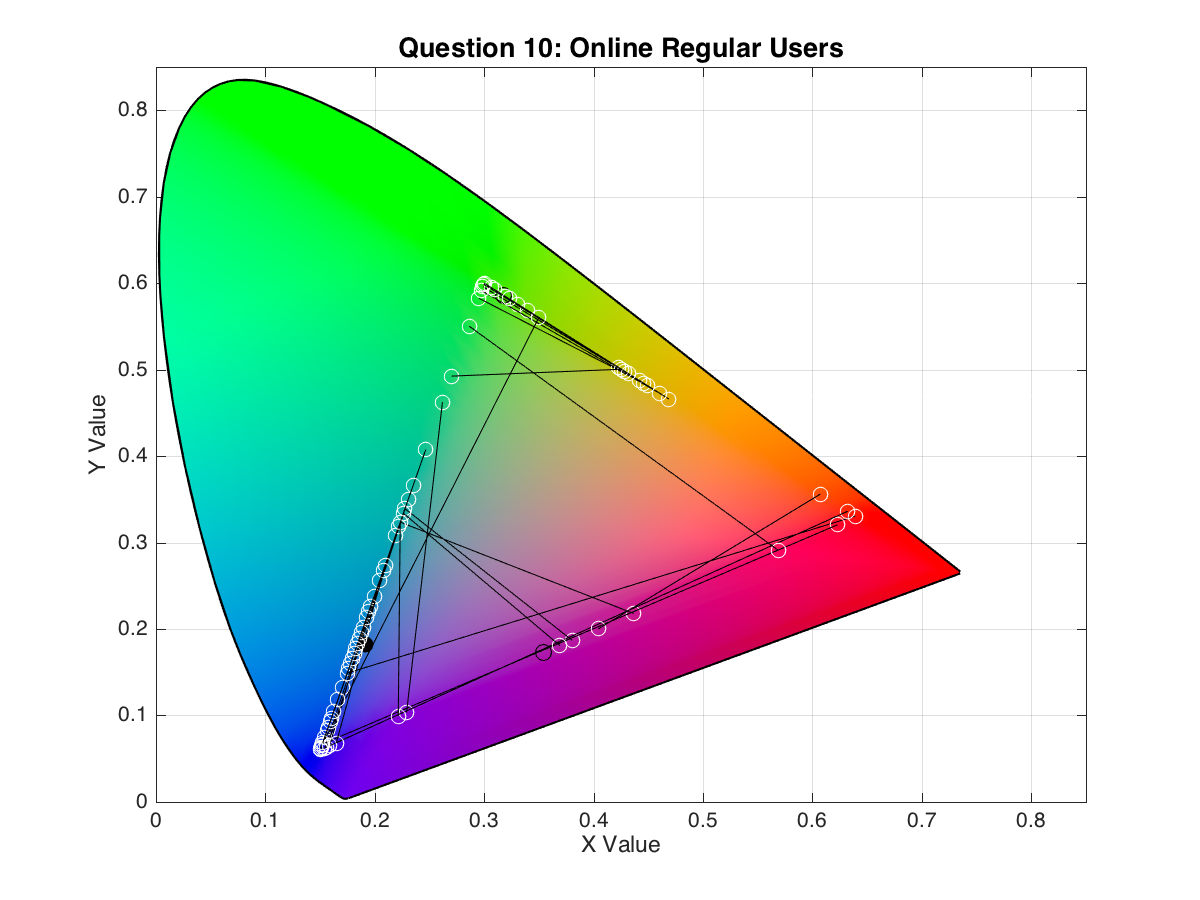
\includegraphics[width=\textwidth]{images/10_online_regularUsers.png}
    \caption[Online Results: Answers for Question 10, from regular users.]{Online Results: Answers for Question 10, from regular users.}
    \label{fig:onlineregular_10}
  \end{minipage}\hfill
  \begin{minipage}{0.48\textwidth}
    \centering
    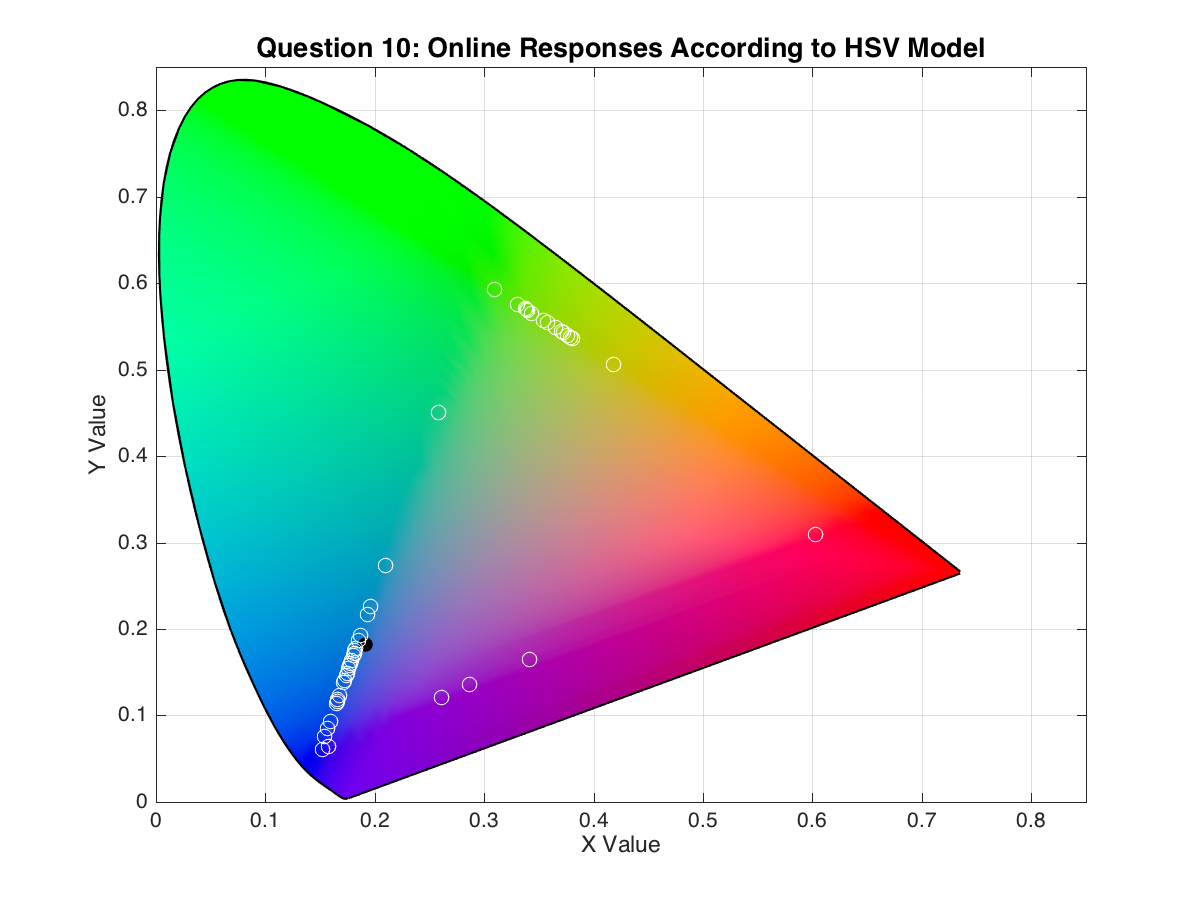
\includegraphics[width=\textwidth]{images/10_online_HSVresponses.png}
    \caption[Online Results: Answers for Question 10, from regular users, mixed in HSV Color Model.]{Online Results: Answers for Question 10, from regular users, mixed in HSV Color Model.}
    \label{fig:onlinehsvregular_10}
  \end{minipage}
\end{figure}
%
\paragraph{\ul{Question Eleven}}
%
As explained in previous question, this one is the second possible output from the blend of \ul{Green and Magenta colors}. This color has no matching color pairs in the other models,
since this color is only obtained in the HSV Color Model. Comparing the results for the HSV Color Model of both questions, mean distances are dramatically lower for question fourteen
($\tilde{x} = 0.06$), whilst the deviation of answers is also lower in question fourteen. \par
%
However, there is an interesting feature: instead of believing in a Green-Magenta blending to produce Orange, \textbf{the users tend to use again Red and Yellow} as on question six,
which explains the low HSV mean value for question eleven.
%
Based on these results, corroborated by the online users, we can conclude \textbf{the orange color is a strongly implemented color in mental models of our users}. The results from
this question can be found in table \ref{table:lab_q11_expected}. These differences can be seen on Figures \ref{fig:onlineregular_11} and \ref{fig:onlinehsvregular_11}, which largely
demonstrates the placement of answer-pairs, and the pairs blended in HSV Color Model.
%
\begin{table}[H]
  \resizebox{\textwidth}{!} {
  \begin{tabular}{lccccccccccccc}
    \hline
    \multicolumn{1}{c}{}                              &                                      & \multicolumn{2}{c}{Expected Colors}                   & \multicolumn{10}{c}{Possible Results}                                                                                                                                                                                                                                                                                        \\ \cline{3-14}
    \multicolumn{1}{c}{\multirow{-2}{*}{Question ID}} & \multirow{-2}{*}{Given Color}        & C1                       & C2                         & \multicolumn{2}{c}{HSV}                                        & \multicolumn{2}{c}{CIE-L*C*h*}                                 & \multicolumn{2}{c}{CMYK}                                       & \multicolumn{2}{c}{RGB}                                        & \multicolumn{2}{c}{CIE-L*a*b*}                                 \\ \hline
    \multicolumn{1}{c}{11}                             & \cellcolor[HTML]{FF8000}(49, 37, 5) & \multicolumn{1}{c|}{Green} & \multicolumn{1}{c|}{Magenta}  & \multicolumn{2}{c|}{\cellcolor[HTML]{FF8000}(49, 37, 5)}      & \multicolumn{2}{c|}{-}       & \multicolumn{2}{c|}{-}       & \multicolumn{2}{c|}{-}       & \multicolumn{2}{c|}{-}       \\ \hline
                                                      & \multicolumn{1}{l}{}                 & \multicolumn{1}{l}{}     & \multicolumn{1}{l}{}       & \multicolumn{1}{c}{$\tilde{x}$} & \multicolumn{1}{c}{$\sigma$} & \multicolumn{1}{c}{$\tilde{x}$} & \multicolumn{1}{c}{$\sigma$} & \multicolumn{1}{c}{$\tilde{x}$} & \multicolumn{1}{c}{$\sigma$} & \multicolumn{1}{c}{$\tilde{x}$} & \multicolumn{1}{c}{$\sigma$} & \multicolumn{1}{c}{$\tilde{x}$} & \multicolumn{1}{c}{$\sigma$} \\ \hline
    \multicolumn{4}{l}{Distance to Objective - Laboratory}                                                                                           & \multicolumn{1}{|c}{0.06}       & \multicolumn{1}{c|}{0.09}    & \multicolumn{1}{|c}{-}       & \multicolumn{1}{c|}{-}    & \multicolumn{1}{|c}{-}       & \multicolumn{1}{c|}{-}    & \multicolumn{1}{|c}{-}       & \multicolumn{1}{c|}{-}    & \multicolumn{1}{|c}{-}       & \multicolumn{1}{c|}{-}    \\
    \multicolumn{4}{l}{Distance to Objective - Online}                                                                                               & \multicolumn{1}{|c}{0.04}        & \multicolumn{1}{c|}{0.06}    & \multicolumn{1}{|c}{-}        & \multicolumn{1}{c|}{-}    & \multicolumn{1}{|c}{-}       & \multicolumn{1}{c|}{-}    & \multicolumn{1}{|c}{-}        & \multicolumn{1}{c|}{-}    & \multicolumn{1}{|c}{-}       & \multicolumn{1}{c|}{-}    \\ \hline
    \end{tabular}}
  \caption[Question 11, with expected Results.]{Question 11, with expected colors, possible results, mean and standard deviation of distances to Objective colors.}
  \label{table:lab_q11_expected}
\end{table}
%
\begin{figure}[htbp]
  \centering
  \begin{minipage}{0.48\textwidth}
    \centering
    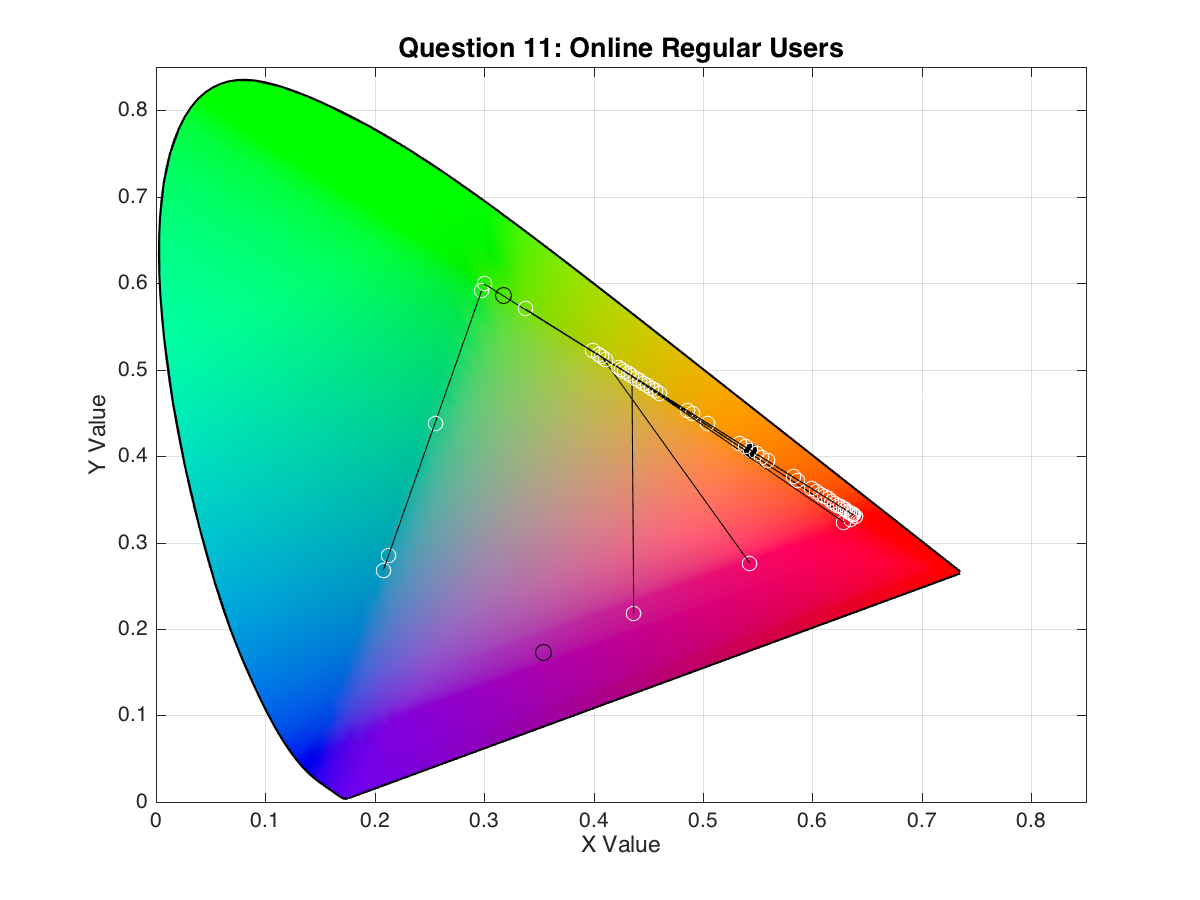
\includegraphics[width=\textwidth]{images/11_online_regularUsers.png}
    \caption[Online Results: Answers for Question 11, from regular users.]{Online Results: Answers for Question 11, from regular users.}
    \label{fig:onlineregular_11}
  \end{minipage}\hfill
  \begin{minipage}{0.48\textwidth}
    \centering
    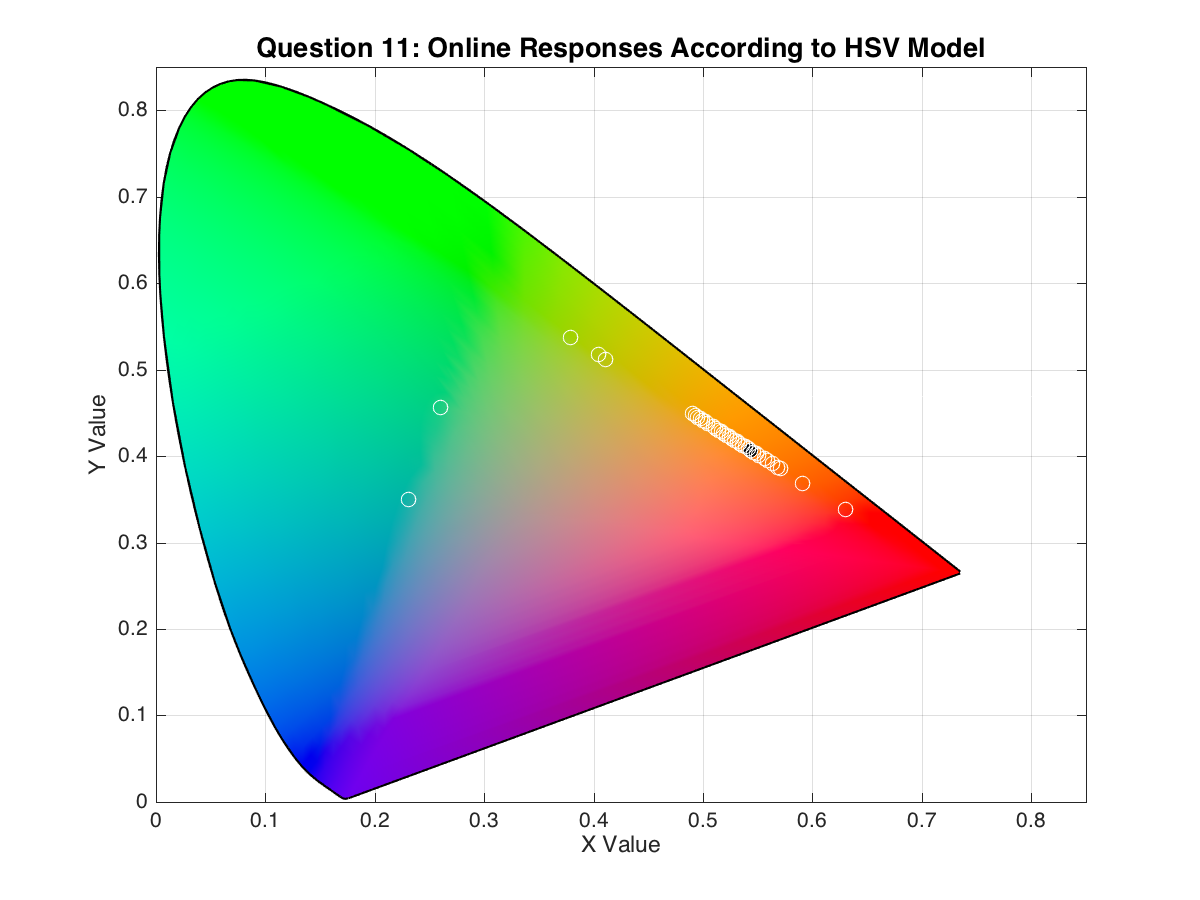
\includegraphics[width=\textwidth]{images/11_online_HSVresponses.png}
    \caption[Online Results: Answers for Question 11, from regular users, mixed in HSV Color Model.]{Online Results: Answers for Question 11, from regular users, mixed in HSV Color Model.}
    \label{fig:onlinehsvregular_11}
  \end{minipage}
\end{figure}
%
\paragraph{\ul{Question Twelve}}
%
This blending question expected \ul{Green and Yellow} colors as response to a tone of \textbf{Green} presented. This green tone is equal to the one presented in question three, therefore
its results are interesting to compare with this question. As observed in Table \ref{table:lab_q12_expected}, when this mixture is blended according to each color model, it generates almost
the same green color, so distances and their statistics are expected to be closer to each other. \par
%
The colors were blended, and again the mean values over distances were calculated, as Table \ref{table:lab_q12_expected} shows. It is observable that HSV Color Model presents,
the lowest mean value for distance to ideal answer ($\tilde{x} = 0.11$), whilst standard deviation for the CMYK Color Model provides the lowest value between both study environments
($\sigma_{lab} = 0.04$, $\sigma_{online} = 0.05$). \par
%
The results show that CIE-L*C*h* the worst-generating values Color Model, having the higher mean value of all models across study environments. There is also the same tendency of RGB,
CIE-L*a*b* and CMYK present closer values between each other. Evaluating the data with the Friedman Test, we can conclude that there are significant differences ($\chi^2 = 71.788$, $p < 0.05$)
between the color models; a Wilcoxon Analysis ($p < 0.05$) does reveal \textbf{there are significant difference between color models}: when analyzing the results for the tests between HSV and other
color models, it presents significant differences between all models except CMYK; the model which consistently presents the larger distances is CIE-L*C*h* against every color model, leading to
statistically significant differences with every other model. \par
%
Comparing the results of this question with number three, we can observe that the later has shorter values: HSV Color Model still presents the best mean values between questions.
The fact that question three has lower values, leads us to conclude that \textbf{mixing Red and Cyan to achieve this green tone is more similar with the users' expectations, than blending a Green and
Yellow color}. Figures \ref{fig:onlinehsvregular_3} and \ref{fig:onlinehsvregular_12} compare the results from both question three and twelve, blended in HSV (the model which yields the best results). \par
%
\begin{table}[H]
  \resizebox{\textwidth}{!} {
  \begin{tabular}{lccccccccccccc}
    \hline
    \multicolumn{1}{c}{}                              &                                      & \multicolumn{2}{c}{Expected Colors}                   & \multicolumn{10}{c}{Possible Results}                                                                                                                                                                                                                                                                                        \\ \cline{3-14}
    \multicolumn{1}{c}{\multirow{-2}{*}{Question ID}} & \multirow{-2}{*}{Given Color}        & C1                       & C2                         & \multicolumn{2}{c}{HSV}                                        & \multicolumn{2}{c}{CIE-L*C*h*}                                 & \multicolumn{2}{c}{CMYK}                                       & \multicolumn{2}{c}{RGB}                                        & \multicolumn{2}{c}{CIE-L*a*b*}                                 \\ \hline
    \multicolumn{1}{c}{12}                             & \cellcolor[HTML]{80FF00}(45, 76, 12) & \multicolumn{1}{c|}{Green} & \multicolumn{1}{c|}{Yellow}  & \multicolumn{2}{c|}{\cellcolor[HTML]{80FF00}(45, 76, 12)}      & \multicolumn{2}{c|}{\cellcolor[HTML]{B1FF00}(54, 81, 13)}       & \multicolumn{2}{c|}{\cellcolor[HTML]{80FF00}(45, 76, 12)}       & \multicolumn{2}{c|}{\cellcolor[HTML]{80FF00}(45, 76, 12)}       & \multicolumn{2}{c|}{\cellcolor[HTML]{AEFF00}(53, 81, 13)}       \\ \hline
                                                      & \multicolumn{1}{l}{}                 & \multicolumn{1}{l}{}     & \multicolumn{1}{l}{}       & \multicolumn{1}{c}{$\tilde{x}$} & \multicolumn{1}{c}{$\sigma$} & \multicolumn{1}{c}{$\tilde{x}$} & \multicolumn{1}{c}{$\sigma$} & \multicolumn{1}{c}{$\tilde{x}$} & \multicolumn{1}{c}{$\sigma$} & \multicolumn{1}{c}{$\tilde{x}$} & \multicolumn{1}{c}{$\sigma$} & \multicolumn{1}{c}{$\tilde{x}$} & \multicolumn{1}{c}{$\sigma$} \\ \hline
    \multicolumn{4}{l}{Distance to Objective - Laboratory}                                                                                           & \multicolumn{1}{|c}{\textbf{0.11}}       & \multicolumn{1}{c|}{0.13}    & \multicolumn{1}{|c}{0.23}       & \multicolumn{1}{c|}{0.07}    & \multicolumn{1}{|c}{0.13}       & \multicolumn{1}{c|}{0.04}    & \multicolumn{1}{|c}{0.15}       & \multicolumn{1}{c|}{0.08}    & \multicolumn{1}{|c}{0.17}       & \multicolumn{1}{c|}{0.07}    \\
    \multicolumn{4}{l}{Distance to Objective - Online}                                                                                               & \multicolumn{1}{|c}{\textbf{0.08}}        & \multicolumn{1}{c|}{0.11}    & \multicolumn{1}{|c}{0.24}        & \multicolumn{1}{c|}{0.06}    & \multicolumn{1}{|c}{0.12}       & \multicolumn{1}{c|}{0.05}    & \multicolumn{1}{|c}{0.13}        & \multicolumn{1}{c|}{0.09}    & \multicolumn{1}{|c}{0.15}       & \multicolumn{1}{c|}{0.09}    \\ \hline
    \end{tabular}}
  \caption[Question 12, with expected Results.]{Question 12, with expected colors, possible results, mean and standard deviation of distances to Objective colors.}
  \label{table:lab_q12_expected}
\end{table}
%
\begin{figure}[htbp]
  \centering
  \begin{minipage}{0.48\textwidth}
    \centering
    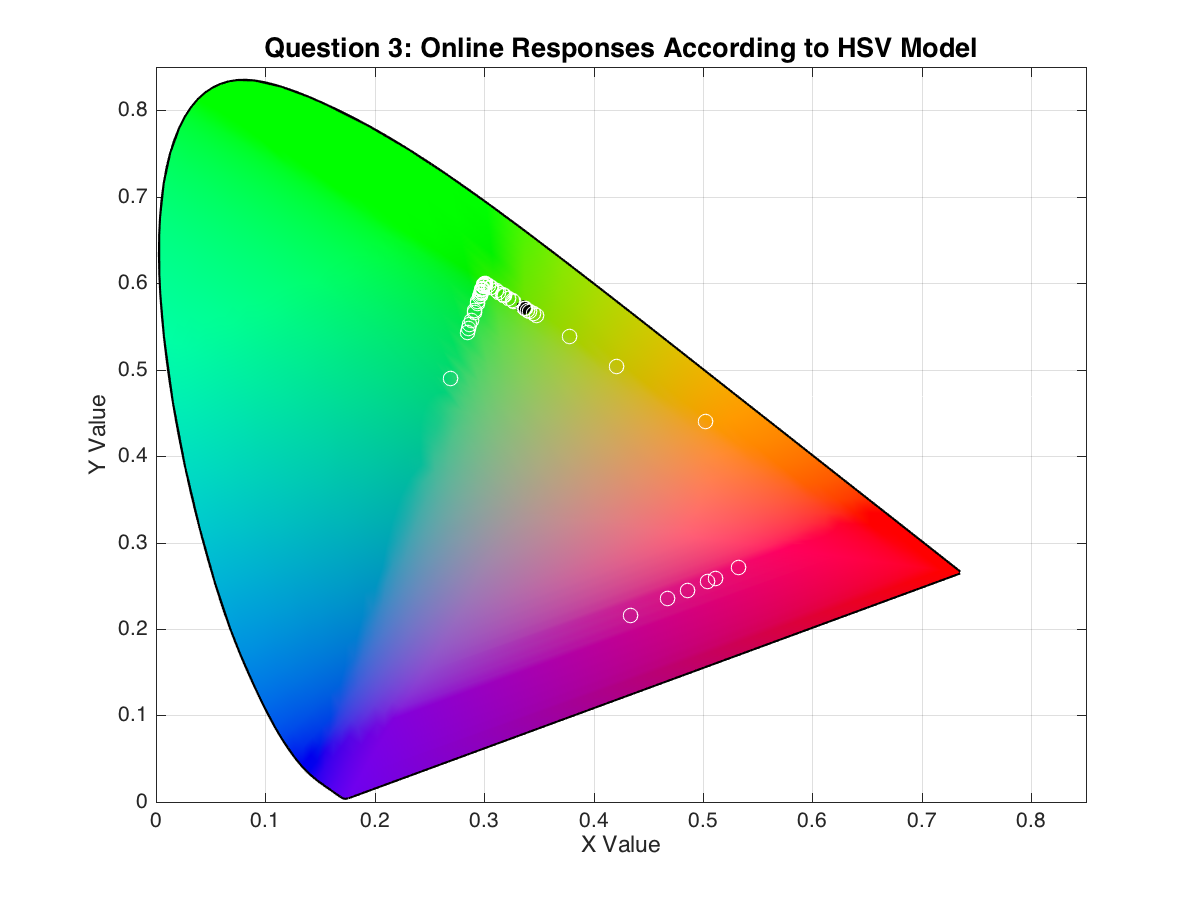
\includegraphics[width=\textwidth]{images/3_online_HSVresponses.png}
    \caption[Online Results: Answers for Question 3, from regular users, mixed in HSV Color Model.]{Online Results: Answers for Question 3, from regular users, mixed in HSV Color Model.}
    \label{fig:onlinehsvregular_3}
  \end{minipage}\hfill
  \begin{minipage}{0.48\textwidth}
    \centering
    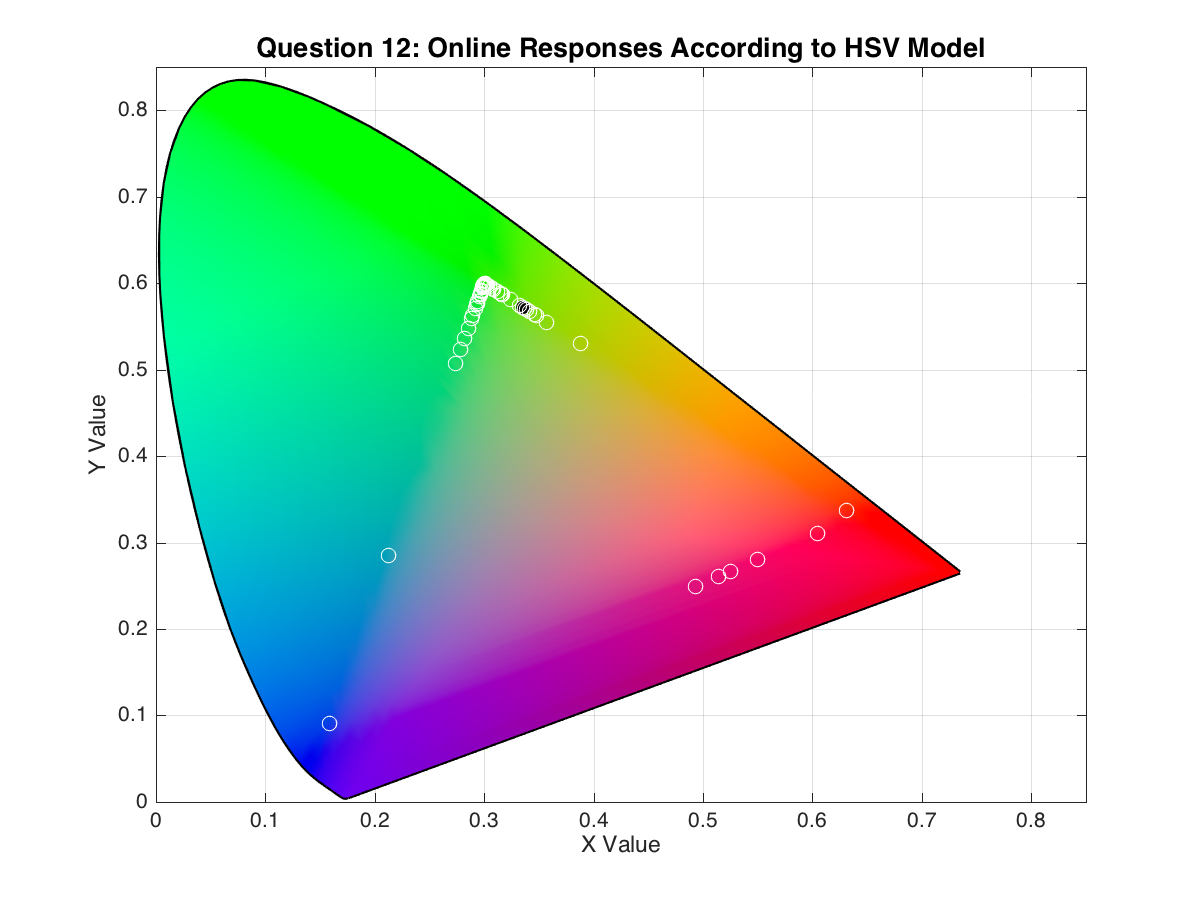
\includegraphics[width=\textwidth]{images/12_online_HSVresponses.png}
    \caption[Online Results: Answers for Question 12, from regular users, mixed in HSV Color Model.]{Online Results: Answers for Question 12, from regular users, mixed in HSV Color Model.}
    \label{fig:onlinehsvregular_12}
  \end{minipage}
\end{figure}
%
\paragraph{\ul{Question Thirteen}}
%
This mixture expected in this question contains \ul{Blue and Cyan} colors as response to a lighter tone of \textbf{Blue}, which was presented. Similar to previous question, this one had
presented a repeated color: this blue shade is equal to the one presented in question ten, therefore its results are interesting to compare with this question. As observed in Table
\ref{table:lab_q13_expected}, when this mixture is blended according to each color model it generates similars colors, except for CIE-L*C*h* that has a ligher blending than others. \par
%
The colors were blended, mean values over distances calculated, as Table \ref{table:lab_q13_expected} shows. It is interesting to see CIE-L*C*h* overcoming the lowest result in the laboratory environment, against other
color models which regularly had best results in previous questions; however, this results are not consistent with the online users, which indicated responses closer to the RGB Color Model
($\sigma_{online} = 0.13$). \par
%
Analyzing the laboratory results, it shows HSV is the worst-generating values Color Model, having the higher mean value ($\tilde{x}_{HSV} = 0.27$) of all models. When comparing it to the online dataset,
HSV, CMYK and CIE-L*a*b* have all the same mean values. Evaluating the data with the Friedman Test, we can conclude that there are significant differences ($\chi^2 = 38.993$, $p < 0.05$)
between the color models on the laboratory results; a Wilcoxon Analysis ($p < 0.05$) does reveal \textbf{there are significant difference between color models}: when analyzing the results for the tests between HSV and other
color models, it presents significant differences between all models except CIE-L*C*h*. \par
%
The fact that online users' data indicate a slight tendency to the RGB Color Model, could be justified as \textbf{the blue color is a primitive of such color model, making it easier to map against
a mental model of color}. \par
%
Comparing the results of this question with number ten, we can observe that this question has shorter HSV value; however we know that HSV was not the lowest mean value on question thirteen
These results leads us to conclude that \textbf{there is insufficient values to ascertain the best color model to achieve this blue tone}. Further studies are required to unveil the
appropriate color model and clarify this matter. Figures \ref{fig:onlinehsvregular_10} and \ref{fig:onlinehsvregular_13} compare the results from both question three and twelve, blended in HSV and RGB respectively,
(the model which yielded the best results in each question). \par
%
\begin{table}[H]
  \resizebox{\textwidth}{!} {
  \begin{tabular}{lccccccccccccc}
    \hline
    \multicolumn{1}{c}{}                              &                                      & \multicolumn{2}{c}{Expected Colors}                   & \multicolumn{10}{c}{Possible Results}                                                                                                                                                                                                                                                                                        \\ \cline{3-14}
    \multicolumn{1}{c}{\multirow{-2}{*}{Question ID}} & \multirow{-2}{*}{Given Color}        & C1                       & C2                         & \multicolumn{2}{c}{HSV}                                        & \multicolumn{2}{c}{CIE-L*C*h*}                                 & \multicolumn{2}{c}{CMYK}                                       & \multicolumn{2}{c}{RGB}                                        & \multicolumn{2}{c}{CIE-L*a*b*}                                 \\ \hline
    \multicolumn{1}{c}{13}                             & \cellcolor[HTML]{0080FF}(26, 23, 98) & \multicolumn{1}{c|}{Blue} & \multicolumn{1}{c|}{Cyan}  & \multicolumn{2}{c|}{\cellcolor[HTML]{0080FF}(26, 23, 98)}      & \multicolumn{2}{c|}{\cellcolor[HTML]{00ACFF}(33, 37, 100)}       & \multicolumn{2}{c|}{\cellcolor[HTML]{0080FF}(26, 23, 98)}       & \multicolumn{2}{c|}{\cellcolor[HTML]{0080FF}(26, 23, 98)}       & \multicolumn{2}{c|}{\cellcolor[HTML]{5792FF}(32, 30, 99)}       \\ \hline
                                                      & \multicolumn{1}{l}{}                 & \multicolumn{1}{l}{}     & \multicolumn{1}{l}{}       & \multicolumn{1}{c}{$\tilde{x}$} & \multicolumn{1}{c}{$\sigma$} & \multicolumn{1}{c}{$\tilde{x}$} & \multicolumn{1}{c}{$\sigma$} & \multicolumn{1}{c}{$\tilde{x}$} & \multicolumn{1}{c}{$\sigma$} & \multicolumn{1}{c}{$\tilde{x}$} & \multicolumn{1}{c}{$\sigma$} & \multicolumn{1}{c}{$\tilde{x}$} & \multicolumn{1}{c}{$\sigma$} \\ \hline
    \multicolumn{4}{l}{Distance to Objective - Laboratory}                                                                                           & \multicolumn{1}{|c}{0.27}       & \multicolumn{1}{c|}{0.16}    & \multicolumn{1}{|c}{\textbf{0.17}}       & \multicolumn{1}{c|}{0.10}    & \multicolumn{1}{|c}{0.19}       & \multicolumn{1}{c|}{0.13}    & \multicolumn{1}{|c}{0.25}       & \multicolumn{1}{c|}{0.16}    & \multicolumn{1}{|c}{0.23}       & \multicolumn{1}{c|}{0.12}    \\
    \multicolumn{4}{l}{Distance to Objective - Online}                                                                                               & \multicolumn{1}{|c}{0.14}        & \multicolumn{1}{c|}{0.16}    & \multicolumn{1}{|c}{0.20}        & \multicolumn{1}{c|}{0.09}    & \multicolumn{1}{|c}{0.14}       & \multicolumn{1}{c|}{0.11}    & \multicolumn{1}{|c}{\textbf{0.13}}        & \multicolumn{1}{c|}{0.15}    & \multicolumn{1}{|c}{0.14}       & \multicolumn{1}{c|}{0.11}    \\ \hline
    \end{tabular}}
  \caption[Question 13, with expected Results.]{Question 13, with expected colors, possible results, mean and standard deviation of distances to Objective colors.}
  \label{table:lab_q13_expected}
\end{table}
%
%
\begin{figure}[htbp]
  \centering
  \begin{minipage}{0.48\textwidth}
    \centering
    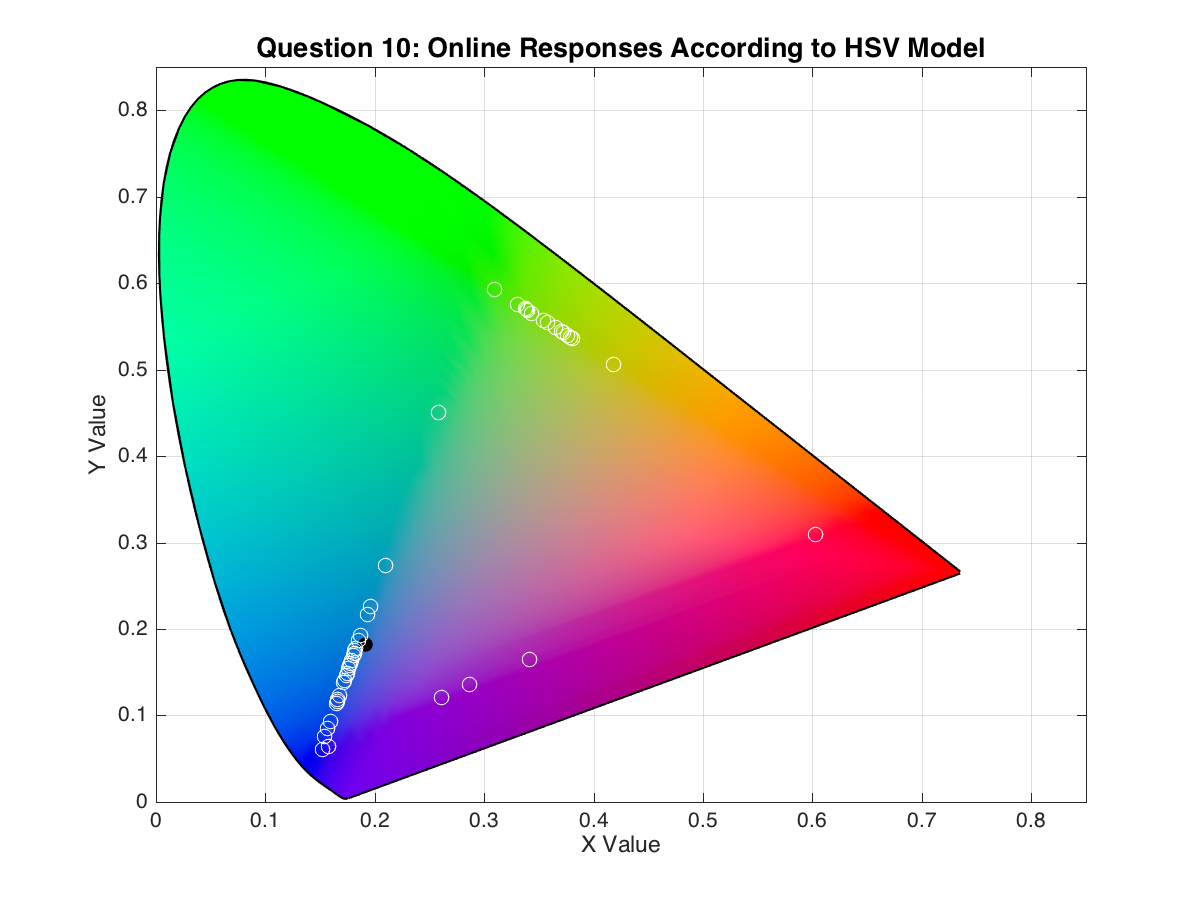
\includegraphics[width=\textwidth]{images/10_online_HSVresponses.png}
    \caption[Online Results: Answers for Question 10, from regular users, mixed in HSV Color Model.]{Online Results: Answers for Question 10, from regular users, mixed in HSV Color Model.}
    \label{fig:onlinehsvregular_10}
  \end{minipage}\hfill
  \begin{minipage}{0.48\textwidth}
    \centering
    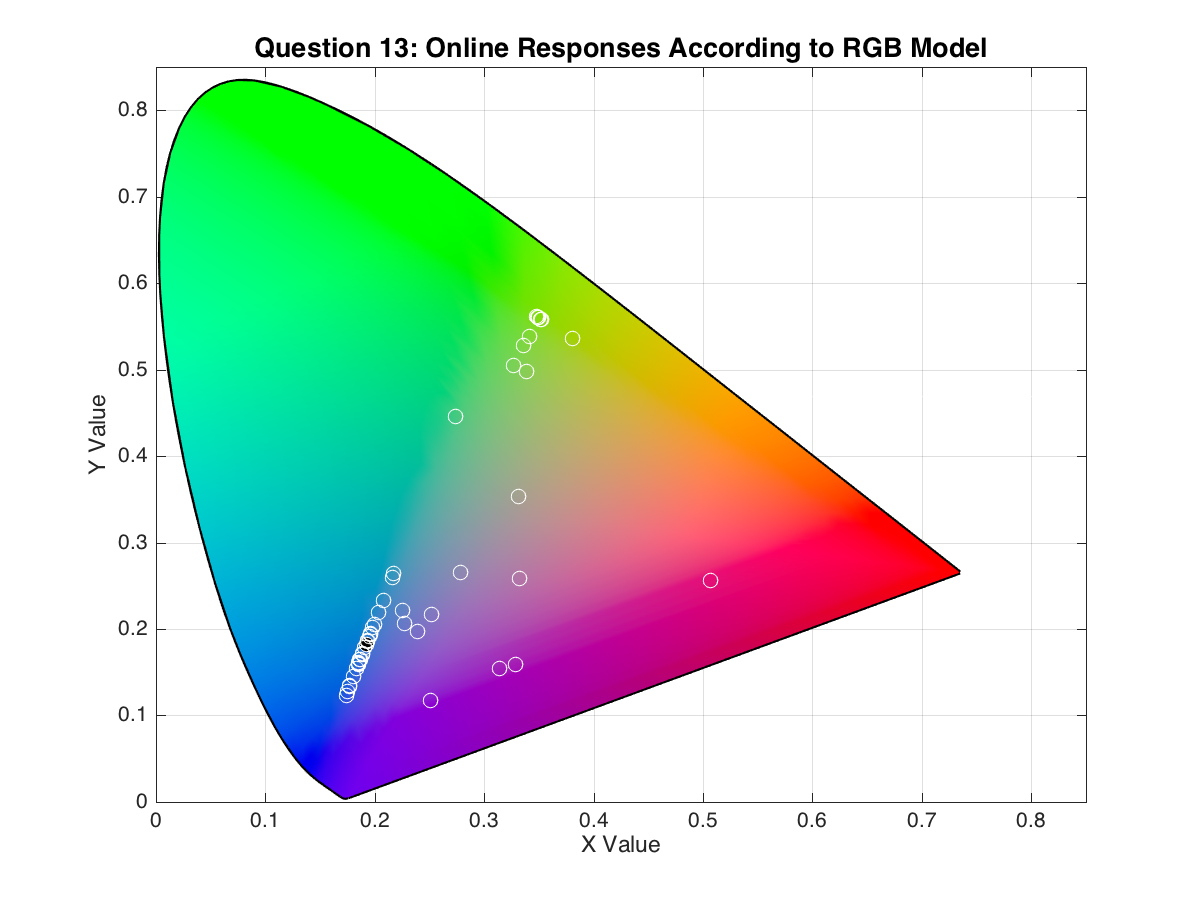
\includegraphics[width=\textwidth]{images/13_online_RGBresponses.png}
    \caption[Online Results: Answers for Question 13, from regular users, mixed in RGB Color Model.]{Online Results: Answers for Question 13, from regular users, mixed in RGB Color Model.}
    \label{fig:onlinergbregular_13}
  \end{minipage}
\end{figure}
%
\paragraph{\ul{Question Fourteen}}
%
This blending question expected \ul{Blue and Magenta} colors as response to a resulting color of \textbf{Purple} (presented to the user). As in Table \ref{table:lab_q14_expected},
when this mixture is blended according to each color model, it generates fairly the same color (precisely the same between HSV, RGB and CMYK). \par
%
The colors were blended, and again the mean values over distances were calculated, as Table \ref{table:lab_q14_expected} shows. It is observable that CMYK Color Model presents,
the lowest mean value for distance to ideal answer ($\tilde{x} = 0.10$ laboratory, and $\tilde{x} = 0.09$ online), whilst standard deviation for the CMYK Color Model is also the
lowest between both study environments presenting exactly the same value. \par
%
The results show that CIE-L*C*h* the worst-generating values Color Model having, by far, the higher mean value of all models across study environments ($\tilde{x} = 0.30$). There is also the same tendency of RGB,
CIE-L*a*b* and HSV present closer values between each other. Evaluating the data with the Friedman Test, we can conclude that there are significant differences ($\chi^2 = 51.726$, $p < 0.05$)
between the color models; a Wilcoxon Analysis ($p < 0.05$) does reveal there are no significant difference between color models: mostly, the significant differences reside in CIE-L*C*h*, when
compared with HSV, CMYK and CIE-L*a*b*. \par
%
Evaluating this question, it is possible to affirm that \textbf{CMYK has the best results when mixing purple, a color derived from magenta}, due to the commitment between the mean value and standard deviation, which
could be justified by the fact that \textbf{magenta is a primitive from such model, combined with the indication shown throughout the study to demonstrate a subtractive mental model of color}.
%
\begin{table}[H]
  \resizebox{\textwidth}{!} {
  \begin{tabular}{lccccccccccccc}
    \hline
    \multicolumn{1}{c}{}                              &                                      & \multicolumn{2}{c}{Expected Colors}                   & \multicolumn{10}{c}{Possible Results}                                                                                                                                                                                                                                                                                        \\ \cline{3-14}
    \multicolumn{1}{c}{\multirow{-2}{*}{Question ID}} & \multirow{-2}{*}{Given Color}        & C1                       & C2                         & \multicolumn{2}{c}{HSV}                                        & \multicolumn{2}{c}{CIE-L*C*h*}                                 & \multicolumn{2}{c}{CMYK}                                       & \multicolumn{2}{c}{RGB}                                        & \multicolumn{2}{c}{CIE-L*a*b*}                                 \\ \hline
    \multicolumn{1}{c}{14}                             & \cellcolor[HTML]{8000FF}(27, 12, 95) & \multicolumn{1}{c|}{Blue} & \multicolumn{1}{c|}{Magenta}  & \multicolumn{2}{c|}{\cellcolor[HTML]{8000FF}(27, 12, 95)}      & \multicolumn{2}{c|}{\cellcolor[HTML]{B000FF}(36, 16, 96)}       & \multicolumn{2}{c|}{\cellcolor[HTML]{8000FF}(27, 12, 95)}       & \multicolumn{2}{c|}{\cellcolor[HTML]{8000FF}(27, 12, 95)}       & \multicolumn{2}{c|}{\cellcolor[HTML]{AB00FF}(35, 16, 96)}       \\ \hline
                                                      & \multicolumn{1}{l}{}                 & \multicolumn{1}{l}{}     & \multicolumn{1}{l}{}       & \multicolumn{1}{c}{$\tilde{x}$} & \multicolumn{1}{c}{$\sigma$} & \multicolumn{1}{c}{$\tilde{x}$} & \multicolumn{1}{c}{$\sigma$} & \multicolumn{1}{c}{$\tilde{x}$} & \multicolumn{1}{c}{$\sigma$} & \multicolumn{1}{c}{$\tilde{x}$} & \multicolumn{1}{c}{$\sigma$} & \multicolumn{1}{c}{$\tilde{x}$} & \multicolumn{1}{c}{$\sigma$} \\ \hline
    \multicolumn{4}{l}{Distance to Objective - Laboratory}                                                                                           & \multicolumn{1}{|c}{0.12}       & \multicolumn{1}{c|}{0.14}    & \multicolumn{1}{|c}{0.30}       & \multicolumn{1}{c|}{0.09}    & \multicolumn{1}{|c}{\textbf{0.10}}       & \multicolumn{1}{c|}{0.05}    & \multicolumn{1}{|c}{0.13}       & \multicolumn{1}{c|}{0.13}    & \multicolumn{1}{|c}{0.13}       & \multicolumn{1}{c|}{0.09}    \\
    \multicolumn{4}{l}{Distance to Objective - Online}                                                                                               & \multicolumn{1}{|c}{0.10}        & \multicolumn{1}{c|}{0.12}    & \multicolumn{1}{|c}{0.29}        & \multicolumn{1}{c|}{0.13}    & \multicolumn{1}{|c}{\textbf{0.09}}       & \multicolumn{1}{c|}{0.05}    & \multicolumn{1}{|c}{0.11}        & \multicolumn{1}{c|}{0.12}    & \multicolumn{1}{|c}{0.12}       & \multicolumn{1}{c|}{0.09}    \\ \hline
    \end{tabular}}
  \caption[Question 14, with expected Results.]{Question 14, with expected colors, possible results, mean and standard deviation of distances to Objective colors.}
  \label{table:lab_q14_expected}
\end{table}
%
\paragraph{\ul{Question Fifteen}}
%
This question \ul{presents a shade of Green color} and expects to receive, the pair \ul{Blue and Yellow}. According to the HSV Color Model, Blue and Yellow are positioned in
opposite angles in the Hue Circle of Colors: therefore, blending these opposite colors that output two different colors. This question should be evaluate along with Question Sixteen, which has
the opposite output. This question also presented a repeated color: this green shade is equal to the one presented in question nine, therefore its results are interesting to compare with this question.\par
%
These two colors, when blended, produce substantitally different colors according to each model interpolation: this question could produce significaaly different results from model to model,
since the users would be clearly indicating which color they would tend to. \par
%
The colors were blended and the mean values over distances were calculated, as Table \ref{table:lab_q15_expected} shows. It is observable that CMYK Color Model presents the lowest mean value
for distance to ideal answer ($\tilde{x} = 0.06$); its standard deviation is also the lowest between both study environments ($\sigma = 0.03$). Though, it is important to analyze this result: since we
are mixing opposite colors, both CMYK and RGB generate a neutral color, which means that the closer the users' answers are from the ideal answers (Blue and Yellow), the shorter the distance on these color
models, and greyer the shade. \textbf{This value, in fact, sustents the result of HSV Color} ($\tilde{x}_{HSV} = 0.09$), which is very acceptable since the answer pairs are very close to the expected one. \par
%
Running the Friedman Test, we can conclude that there are significant differences ($\chi^2 = 63.068$, $p < 0.05$) between the color models; a Wilcoxon Analysis ($p < 0.05$) reveals that
there are statistically different results among all color models, except for \ul{HSV and RGB} and \ul{HSV and CIE-L*a*b*}, which do not have statistically signifcant differences. \par
%
Comparing the results of this question with number nine, we can observe that this question has shorter values: HSV Color Model still presents the best mean values between questions, and deviations of question 15
answers are lower for all models against question 9. This fact leads us to conclude that \textbf{mixing Blue and Cyan to achieve this green shade is more similar with the users' expectations, than blending a Green and
Cyan color}. Figures \ref{fig:onlinehsvregular_9} and \ref{fig:onlinehsvregular_15} compare the results from both question nine and fifteen, blended in HSV (the model which yields the best results). \par
%
HSV has statistically different results from other color models, therefore concluding that \textbf{HSV has the best solution for this blending}, according to users' responses. It is necessary to analyze
pairwise the next question to evaluate the efectiveness of this output, for Blue and Yellow colors blending. \par
%
\begin{table}[H]
  \resizebox{\textwidth}{!} {
  \begin{tabular}{lccccccccccccc}
    \hline
    \multicolumn{1}{c}{}                              &                                      & \multicolumn{2}{c}{Expected Colors}                   & \multicolumn{10}{c}{Possible Results}                                                                                                                                                                                                                                                                                        \\ \cline{3-14}
    \multicolumn{1}{c}{\multirow{-2}{*}{Question ID}} & \multirow{-2}{*}{Given Color}        & C1                       & C2                         & \multicolumn{2}{c}{HSV}                                        & \multicolumn{2}{c}{CIE-L*C*h*}                                 & \multicolumn{2}{c}{CMYK}                                       & \multicolumn{2}{c}{RGB}                                        & \multicolumn{2}{c}{CIE-L*a*b*}                                 \\ \hline
    \multicolumn{1}{c}{15}                             & \cellcolor[HTML]{00FF80}(40, 73, 32) & \multicolumn{1}{c|}{Blue} & \multicolumn{1}{c|}{Yellow}  & \multicolumn{2}{c|}{\cellcolor[HTML]{00FF80}(40, 73, 32)}      & \multicolumn{2}{c|}{\cellcolor[HTML]{FF0050}(43, 22, 10)}       & \multicolumn{2}{c|}{\cellcolor[HTML]{808080}(21, 22, 24)}       & \multicolumn{2}{c|}{\cellcolor[HTML]{808080}(21, 22, 24)}       & \multicolumn{2}{c|}{\cellcolor[HTML]{CA8AAA}(41, 34, 42)}       \\ \hline
                                                      & \multicolumn{1}{l}{}                 & \multicolumn{1}{l}{}     & \multicolumn{1}{l}{}       & \multicolumn{1}{c}{$\tilde{x}$} & \multicolumn{1}{c}{$\sigma$} & \multicolumn{1}{c}{$\tilde{x}$} & \multicolumn{1}{c}{$\sigma$} & \multicolumn{1}{c}{$\tilde{x}$} & \multicolumn{1}{c}{$\sigma$} & \multicolumn{1}{c}{$\tilde{x}$} & \multicolumn{1}{c}{$\sigma$} & \multicolumn{1}{c}{$\tilde{x}$} & \multicolumn{1}{c}{$\sigma$} \\ \hline
    \multicolumn{4}{l}{Distance to Objective - Laboratory}                                                                                           & \multicolumn{1}{|c}{0.09}       & \multicolumn{1}{c|}{0.04}    & \multicolumn{1}{|c}{0.30}       & \multicolumn{1}{c|}{0.08}    & \multicolumn{1}{|c}{\textbf{0.06}}       & \multicolumn{1}{c|}{0.03}    & \multicolumn{1}{|c}{0.11}       & \multicolumn{1}{c|}{0.05}    & \multicolumn{1}{|c}{0.13}       & \multicolumn{1}{c|}{0.06}    \\
    \multicolumn{4}{l}{Distance to Objective - Online}                                                                                               & \multicolumn{1}{|c}{0.11}        & \multicolumn{1}{c|}{0.08}    & \multicolumn{1}{|c}{0.30}        & \multicolumn{1}{c|}{0.07}    & \multicolumn{1}{|c}{\textbf{0.06}}       & \multicolumn{1}{c|}{0.03}    & \multicolumn{1}{|c}{0.11}        & \multicolumn{1}{c|}{0.04}    & \multicolumn{1}{|c}{0.13}       & \multicolumn{1}{c|}{0.06}    \\ \hline
    \end{tabular}}
  \caption[Question 15, with expected Results.]{Question 15, with expected colors, possible results, mean and standard deviation of distances to Objective colors.}
  \label{table:lab_q15_expected}
\end{table}
%
\begin{figure}[htbp]
  \centering
  \begin{minipage}{0.48\textwidth}
    \centering
    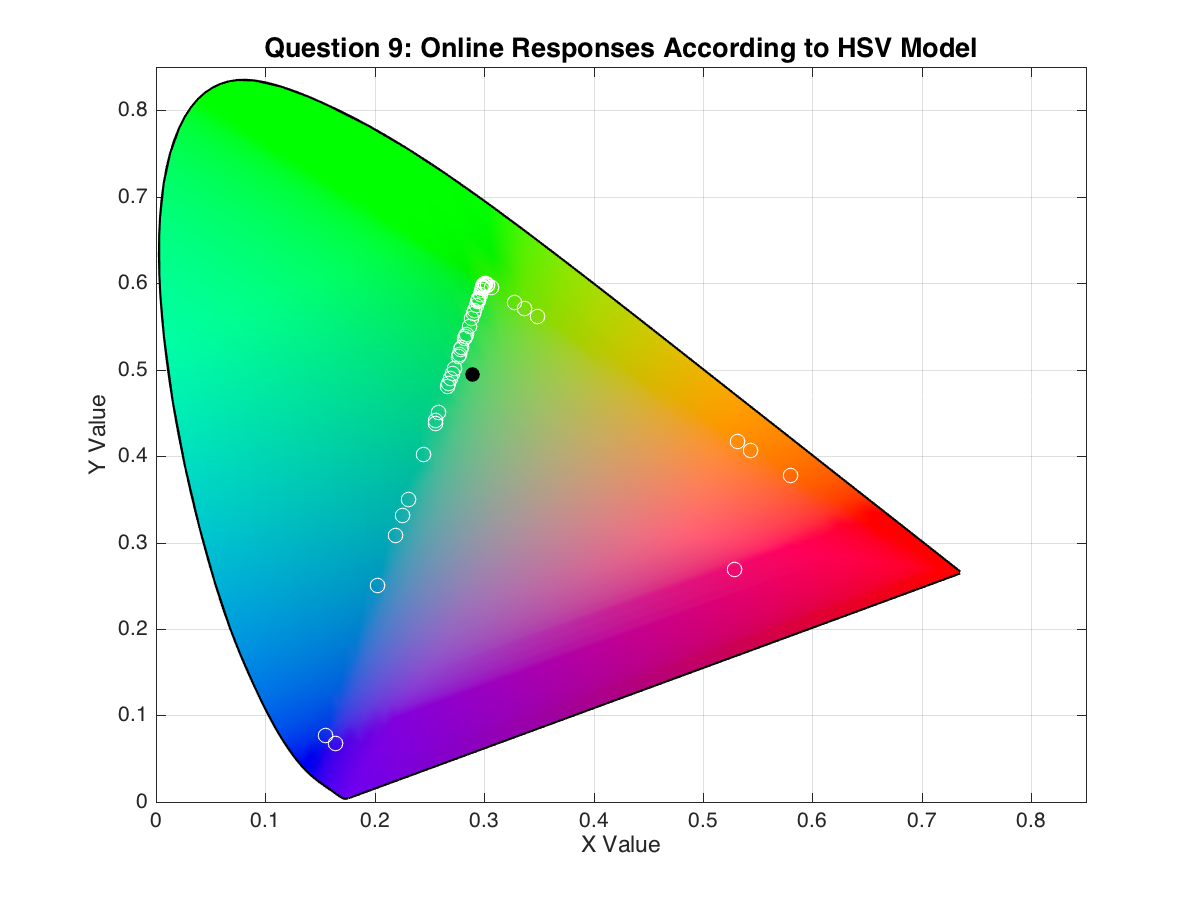
\includegraphics[width=\textwidth]{images/9_online_HSVresponses.png}
    \caption[Online Results: Answers for Question 9, from regular users, mixed in HSV Color Model.]{Online Results: Answers for Question 9, from regular users, mixed in HSV Color Model.}
    \label{fig:onlinehsvregular_9}
  \end{minipage}\hfill
  \begin{minipage}{0.48\textwidth}
    \centering
    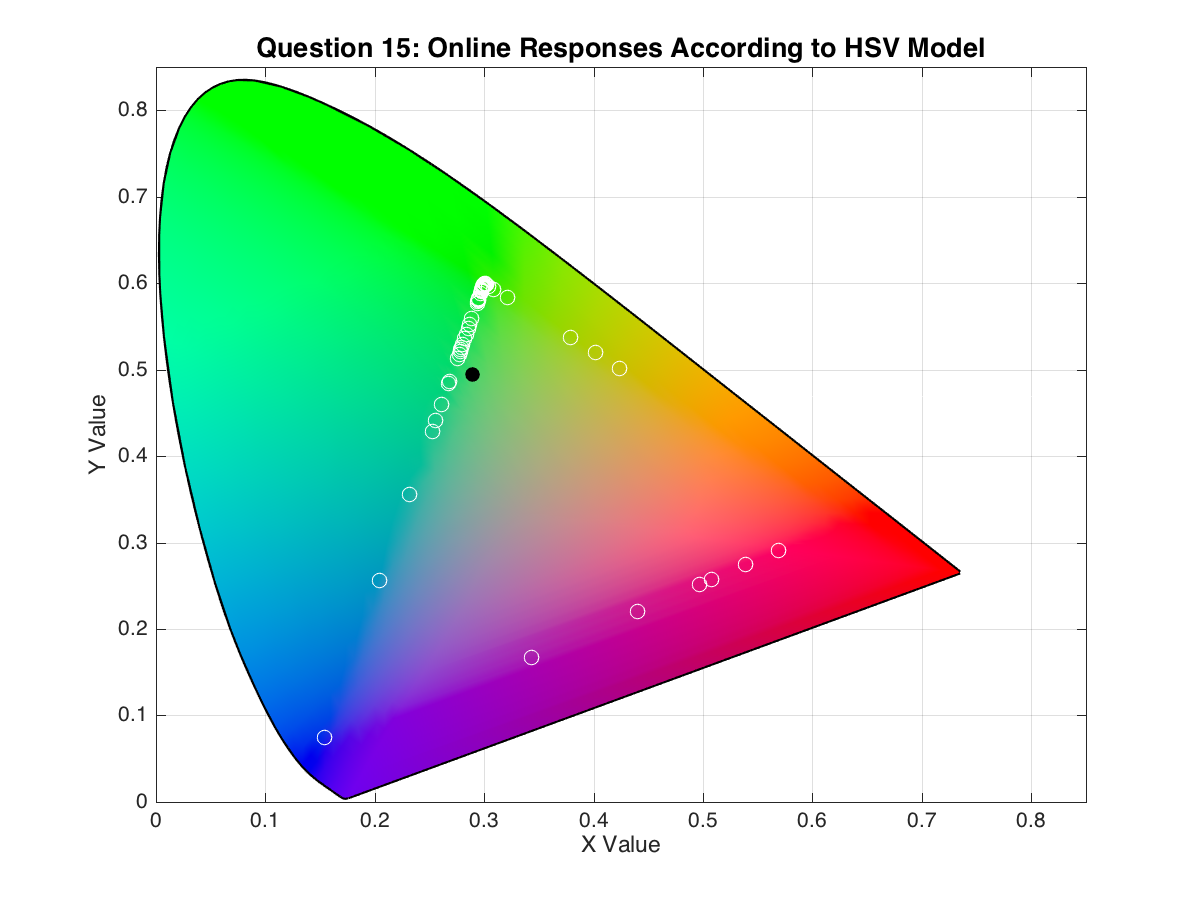
\includegraphics[width=\textwidth]{images/15_online_HSVresponses.png}
    \caption[Online Results: Answers for Question 15, from regular users, mixed in HSV Color Model.]{Online Results: Answers for Question 15, from regular users, mixed in HSV Color Model.}
    \label{fig:onlinehsvregular_15}
  \end{minipage}
\end{figure}
%
\paragraph{\ul{Question Sixteen}}
%
As explained in previous question, this one is the second possible output from the blend of \ul{Blue and Yellow colors}. This color has no matching color pairs in the other models,
since this color is only obtained in the HSV Color Model. Comparing the results for the HSV Color Model of both questions, mean distances are largely high for question sixteen
($\tilde{x}_{lab} = 0.21$, $\tilde{x}_{online} = 0.19$), whilst the deviation of answers is also lower in question fifteen. \par
%
Whilst the color presented was fairly similar with Magenta, the users tended to answer with Red-Blue pair of colors (which, as seen on question two, produces magenta according
to the HSV Color Model). \par
%
Based on these results, corroborated by the online users, we can conclude that \textbf{blending Blue and Yellow, according to users' mental model of color, produces Green instead of Magenta}. It is also
possible to conclude that \textbf{to produce Magenta, according to user's mental model of color, it is needed to blend Red and Blue}. The results from
this question can be found in table \ref{table:lab_q16_expected}. These differences can be seen on Figures \ref{fig:onlineregular_16} and \ref{fig:onlinehsvregular_16}, which largely
demonstrates the placement of answer-pairs, and the pairs blended in HSV Color Model.
%
\begin{table}[H]
  \resizebox{\textwidth}{!} {
  \begin{tabular}{lccccccccccccc}
    \hline
    \multicolumn{1}{c}{}                              &                                      & \multicolumn{2}{c}{Expected Colors}                   & \multicolumn{10}{c}{Possible Results}                                                                                                                                                                                                                                                                                        \\ \cline{3-14}
    \multicolumn{1}{c}{\multirow{-2}{*}{Question ID}} & \multirow{-2}{*}{Given Color}        & C1                       & C2                         & \multicolumn{2}{c}{HSV}                                        & \multicolumn{2}{c}{CIE-L*C*h*}                                 & \multicolumn{2}{c}{CMYK}                                       & \multicolumn{2}{c}{RGB}                                        & \multicolumn{2}{c}{CIE-L*a*b*}                                 \\ \hline
    \multicolumn{1}{c}{16}                             & \cellcolor[HTML]{FF007F}(45, 23, 22) & \multicolumn{1}{c|}{Blue} & \multicolumn{1}{c|}{Yellow}  & \multicolumn{2}{c|}{\cellcolor[HTML]{FF007F}(45, 23, 22)}      & \multicolumn{2}{c|}{-}       & \multicolumn{2}{c|}{-}       & \multicolumn{2}{c|}{}       & \multicolumn{2}{c|}{}       \\ \hline
                                                      & \multicolumn{1}{l}{}                 & \multicolumn{1}{l}{}     & \multicolumn{1}{l}{}       & \multicolumn{1}{c}{$\tilde{x}$} & \multicolumn{1}{c}{$\sigma$} & \multicolumn{1}{c}{$\tilde{x}$} & \multicolumn{1}{c}{$\sigma$} & \multicolumn{1}{c}{$\tilde{x}$} & \multicolumn{1}{c}{$\sigma$} & \multicolumn{1}{c}{$\tilde{x}$} & \multicolumn{1}{c}{$\sigma$} & \multicolumn{1}{c}{$\tilde{x}$} & \multicolumn{1}{c}{$\sigma$} \\ \hline
    \multicolumn{4}{l}{Distance to Objective - Laboratory}                                                                                           & \multicolumn{1}{|c}{0.21}       & \multicolumn{1}{c|}{0.10}    & \multicolumn{1}{|c}{-}       & \multicolumn{1}{c|}{-}    & \multicolumn{1}{|c}{-}       & \multicolumn{1}{c|}{-}    & \multicolumn{1}{|c}{-}       & \multicolumn{1}{c|}{-}    & \multicolumn{1}{|c}{-}       & \multicolumn{1}{c|}{-}    \\
    \multicolumn{4}{l}{Distance to Objective - Online}                                                                                               & \multicolumn{1}{|c}{0.19}        & \multicolumn{1}{c|}{0.12}    & \multicolumn{1}{|c}{-}        & \multicolumn{1}{c|}{-}    & \multicolumn{1}{|c}{-}       & \multicolumn{1}{c|}{-}    & \multicolumn{1}{|c}{-}        & \multicolumn{1}{c|}{-}    & \multicolumn{1}{|c}{-}       & \multicolumn{1}{c|}{-}    \\ \hline
    \end{tabular}}
  \caption[Question 16, with expected Results.]{Question 16, with expected colors, possible results, mean and standard deviation of distances to Objective colors.}
  \label{table:lab_q16_expected}
\end{table}
%
\begin{figure}[htbp]
  \centering
  \begin{minipage}{0.48\textwidth}
    \centering
    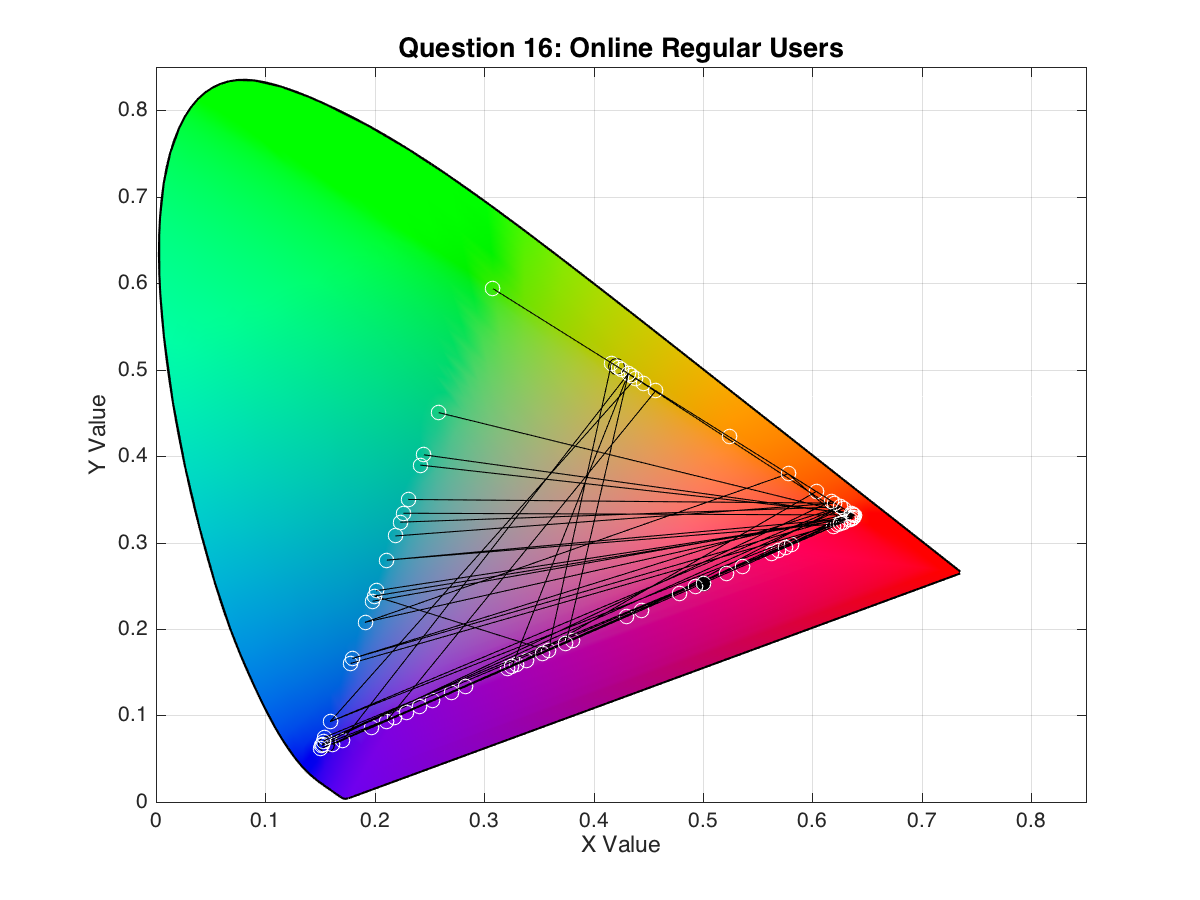
\includegraphics[width=\textwidth]{images/16_online_regularUsers.png}
    \caption[Online Results: Answers for Question 16, from regular users.]{Online Results: Answers for Question 16, from regular users.}
    \label{fig:onlineregular_16}
  \end{minipage}\hfill
  \begin{minipage}{0.48\textwidth}
    \centering
    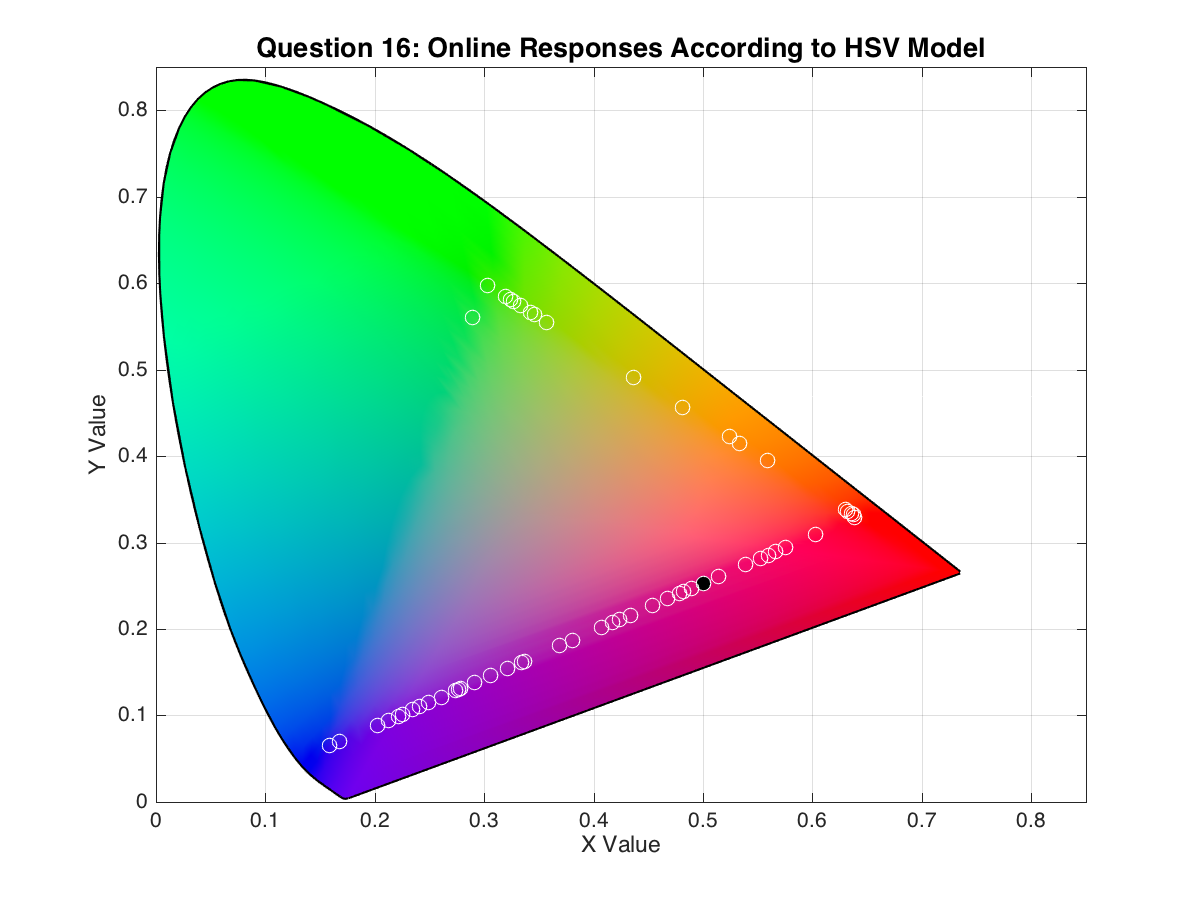
\includegraphics[width=\textwidth]{images/16_online_HSVresponses.png}
    \caption[Online Results: Answers for Question 16, from regular users, mixed in HSV Color Model.]{Online Results: Answers for Question 16, from regular users, mixed in HSV Color Model.}
    \label{fig:onlinehsvregular_16}
  \end{minipage}
\end{figure}
%
\paragraph{\ul{Question Seventeen}}
%
The last question in which we ask the user to indicate two colors is this: we expected to receive \ul{Cyan and Yellow} colors as response, to a resulting color of \textbf{Green}
(presented to the user). As in Table \ref{table:lab_q17_expected}, when this mixture is blended according to each color model, it generates fairly the same color (precisely the same between
RGB and CMYK). \par
%
The colors were blended, and mean values over distances were calculated. It is observable that CMYK Color Model presents the lowest mean value for distance to ideal answer ($\tilde{x} = 0.05$
laboratory, and $\tilde{x} = 0.05$ online), whilst standard deviation for the CMYK Color Model is also the lowest between both study environments presenting exactly the same value. \par
%
The results show that CIE-L*C*h* the worst-generating values Color Model having the higher mean value of all models across study environments ($\tilde{x} = 0.16$), which is consistent with the
entire user study. There is also the tendency of RGB and CIE-L*a*b* to present closer values between each other. Evaluating the data with the Friedman Test, we can conclude that there are significant
differences ($\chi^2 = 86.654$, $p < 0.05$) between the color models; a Wilcoxon Analysis ($p < 0.05$) does reveal there are clearly significant difference between color models: mostly, every color model
has significant differences between each other, except for HSV-CMYK, and RGB-CIE-L*a*b* which in fact present no statistically significant differences. \par
%
Evaluating this question, it is possible to affirm that \textbf{CMYK has the best results when cyan and yellow}, due to the commitment between the mean value and standard deviation, which
could be justified by the fact that \textbf{cyan and yellow are primitives from such model, combined with the indication shown throughout the study to demonstrate a subtractive mental model of color}. \par
%
\begin{table}[H]
  \resizebox{\textwidth}{!} {
  \begin{tabular}{lccccccccccccc}
    \hline
    \multicolumn{1}{c}{}                              &                                      & \multicolumn{2}{c}{Expected Colors}                   & \multicolumn{10}{c}{Possible Results}                                                                                                                                                                                                                                                                                        \\ \cline{3-14}
    \multicolumn{1}{c}{\multirow{-2}{*}{Question ID}} & \multirow{-2}{*}{Given Color}        & C1                       & C2                         & \multicolumn{2}{c}{HSV}                                        & \multicolumn{2}{c}{CIE-L*C*h*}                                 & \multicolumn{2}{c}{CMYK}                                       & \multicolumn{2}{c}{RGB}                                        & \multicolumn{2}{c}{CIE-L*a*b*}                                 \\ \hline
    \multicolumn{1}{c}{17}                             & \cellcolor[HTML]{00FF00}(36, 72, 13) & \multicolumn{1}{c|}{Cyan} & \multicolumn{1}{c|}{Yellow}  & \multicolumn{2}{c|}{\cellcolor[HTML]{00FF00}(36, 72, 13)}      & \multicolumn{2}{c|}{\cellcolor[HTML]{6EFFA3}(49, 77, 47)}       & \multicolumn{2}{c|}{\cellcolor[HTML]{80FF80}(49, 78, 33)}       & \multicolumn{2}{c|}{\cellcolor[HTML]{80FF80}(49, 78, 33)}       & \multicolumn{2}{c|}{\cellcolor[HTML]{C4FF9E}(66, 87, 46)}       \\ \hline
                                                      & \multicolumn{1}{l}{}                 & \multicolumn{1}{l}{}     & \multicolumn{1}{l}{}       & \multicolumn{1}{c}{$\tilde{x}$} & \multicolumn{1}{c}{$\sigma$} & \multicolumn{1}{c}{$\tilde{x}$} & \multicolumn{1}{c}{$\sigma$} & \multicolumn{1}{c}{$\tilde{x}$} & \multicolumn{1}{c}{$\sigma$} & \multicolumn{1}{c}{$\tilde{x}$} & \multicolumn{1}{c}{$\sigma$} & \multicolumn{1}{c}{$\tilde{x}$} & \multicolumn{1}{c}{$\sigma$} \\ \hline
    \multicolumn{4}{l}{Distance to Objective - Laboratory}                                                                                           & \multicolumn{1}{|c}{0.07}       & \multicolumn{1}{c|}{0.10}    & \multicolumn{1}{|c}{0.16}       & \multicolumn{1}{c|}{0.06}    & \multicolumn{1}{|c}{\textbf{0.05}}       & \multicolumn{1}{c|}{0.02}    & \multicolumn{1}{|c}{0.10}       & \multicolumn{1}{c|}{0.06}    & \multicolumn{1}{|c}{0.11}       & \multicolumn{1}{c|}{0.05}    \\
    \multicolumn{4}{l}{Distance to Objective - Online}                                                                                               & \multicolumn{1}{|c}{0.08}        & \multicolumn{1}{c|}{0.13}    & \multicolumn{1}{|c}{0.17}        & \multicolumn{1}{c|}{0.06}    & \multicolumn{1}{|c}{\textbf{0.05}}       & \multicolumn{1}{c|}{0.03}    & \multicolumn{1}{|c}{0.10}        & \multicolumn{1}{c|}{0.06}    & \multicolumn{1}{|c}{0.11}       & \multicolumn{1}{c|}{0.05}    \\ \hline
    \end{tabular}}
  \caption[Question 17, with expected Results.]{Question 17, with expected colors, possible results, mean and standard deviation of distances to Objective colors.}
  \label{table:lab_q17_expected}
\end{table}
%
%
%%%%%%%%%%%%%%%%%%%%%%%%%%%%%%%%%%%%%%%%%%%%%%%%%%%%%%%%%%%%%%%%%%%%%%%%%%%%%%%%
%
\subsubsection{Analyzing Color Models}
\label{subsubsec:models_analyzing}
%
Now that we have broke down the results for each question, it is important to evaluate the values according to each color model. Based on table \ref{table:colormodels_distances_labonline},
which presents the mean values for each color model decomposed by question, we can run descriptive statistics over its column and produce table \ref{table:colormodels_distances_labonline_statistics} that
is going to be helpul when inspecting the results \emph{per} color model. We have also gathered the results from the previous section, displaying the three best and worst results of each color model, identified as green and red,
respectively: this information is condensed in table \ref{table:colormodels_distances_questions_statistics}. \par
%
\begin{table}[htbp]
  \resizebox{\textwidth}{!} {
  \begin{tabular}{@{}ccccccccccc@{}}
    \toprule
                                  & \multicolumn{2}{c}{HSV}                                                                                                                              & \multicolumn{2}{c}{CIE-L*C*h*}                                                                                               & \multicolumn{2}{c}{CMYK}                                                                                                     & \multicolumn{2}{c}{RGB}                                                                                                      & \multicolumn{2}{c}{CIE-L*a*b*}                                                                                               \\ \cmidrule(l){2-11}
    \multirow{-2}{*}{Question ID} & Mean ($\tilde{x}$)                                                                  & Std-Dev ($\sigma$)                                             & Mean ($\tilde{x}$)                                           & Std-Dev ($\sigma$)                                            & Mean ($\tilde{x}$)                                           & Std-Dev ($\sigma$)                                            & Mean ($\tilde{x}$)                                           & Std-Dev ($\sigma$)                                            & \multicolumn{1}{c|}{Mean ($\tilde{x}$)}                      & \multicolumn{1}{c|}{Std-Dev ($\sigma$)}                       \\ \midrule
    \multicolumn{1}{c|}{1}        & \multicolumn{1}{c|}{0.1258}                                                         & \multicolumn{1}{c||}{\cellcolor[HTML]{32CB00}\textbf{0.08275}}  & \multicolumn{1}{c|}{0.2042}                                  & \multicolumn{1}{c||}{\cellcolor[HTML]{32CB00}\textbf{0.0644}}  & \multicolumn{1}{c|}{0.0926}                                  & \multicolumn{1}{c||}{0.06118}                                  & \multicolumn{1}{c|}{0.1237}                                  & \multicolumn{1}{c||}{0.07925}                                  & \multicolumn{1}{c|}{0.1232}                                  & \multicolumn{1}{c|}{0.0807}                                   \\ \midrule
    \multicolumn{1}{c|}{2}        & \multicolumn{1}{c|}{\cellcolor[HTML]{FD6864}\textbf{0.2173}}                        & \multicolumn{1}{c||}{0.13014}                                   & \multicolumn{1}{c|}{\cellcolor[HTML]{32CB00}\textbf{0.1573}} & \multicolumn{1}{c||}{0.09445}                                  & \multicolumn{1}{c|}{0.106}                                   & \multicolumn{1}{c||}{0.05642}                                  & \multicolumn{1}{c|}{\cellcolor[HTML]{FD6864}\textbf{0.166}}  & \multicolumn{1}{c||}{0.10521}                                  & \multicolumn{1}{c|}{0.156}                                   & \multicolumn{1}{c|}{0.08399}                                  \\ \midrule \midrule
    \multicolumn{1}{c|}{3}        & \multicolumn{1}{c|}{0.0941}                                                         & \multicolumn{1}{c||}{0.12308}                                   & \multicolumn{1}{c|}{0.23}                                    & \multicolumn{1}{c||}{\cellcolor[HTML]{32CB00}\textbf{0.05855}} & \multicolumn{1}{c|}{0.0609}                                  & \multicolumn{1}{c||}{\cellcolor[HTML]{32CB00}\textbf{0.03379}}                                  & \multicolumn{1}{c|}{0.1114}                                  & \multicolumn{1}{c||}{\cellcolor[HTML]{32CB00}\textbf{0.06034}}                                  & \multicolumn{1}{c|}{0.1227}                                  & \multicolumn{1}{c|}{\cellcolor[HTML]{32CB00}\textbf{0.03918}} \\ \midrule
    \multicolumn{1}{c|}{4}        & \multicolumn{1}{c|}{0.1162}                                                         & \multicolumn{1}{c||}{0.12975}                                   & \multicolumn{8}{c}{}                                                                                                                                                                                                                                                                                                                                                                                                                                                                                                      \\ \midrule \midrule
    \multicolumn{1}{c|}{5}        & \multicolumn{1}{c|}{0.1683}                                                         & \multicolumn{1}{c||}{0.10113}                                   & \multicolumn{1}{c|}{\cellcolor[HTML]{32CB00}\textbf{0.15}}   & \multicolumn{1}{c||}{0.08}                                     & \multicolumn{1}{c|}{\cellcolor[HTML]{FD6864}\textbf{0.1322}} & \multicolumn{1}{c||}{0.06787}                                  & \multicolumn{1}{c|}{0.1389}                                  & \multicolumn{1}{c||}{0.09106}                                  & \multicolumn{1}{c|}{0.135}                                   & \multicolumn{1}{c|}{0.07579}                                  \\ \midrule
    \multicolumn{1}{c|}{6}        & \multicolumn{1}{c|}{\cellcolor[HTML]{32CB00}{\color[HTML]{000000} \textbf{0.0741}}} & \multicolumn{1}{c||}{0.10418}                                   & \multicolumn{1}{c|}{\cellcolor[HTML]{32CB00}\textbf{0.1332}} & \multicolumn{1}{c||}{0.08671}                                  & \multicolumn{1}{c|}{\cellcolor[HTML]{32CB00}\textbf{0.0577}} & \multicolumn{1}{c||}{0.06164}                                  & \multicolumn{1}{c|}{\cellcolor[HTML]{32CB00}\textbf{0.0777}} & \multicolumn{1}{c||}{0.0973}                                   & \multicolumn{1}{c|}{\cellcolor[HTML]{32CB00}\textbf{0.0509}} & \multicolumn{1}{c|}{0.07374}                                  \\ \midrule
    \multicolumn{1}{c|}{7}        & \multicolumn{1}{c|}{0.1577}                                                         & \multicolumn{1}{c||}{\cellcolor[HTML]{FD6864}\textbf{0.20679}}  & \multicolumn{1}{c|}{0.2323}                                  & \multicolumn{1}{c||}{\cellcolor[HTML]{FD6864}\textbf{0.10038}}                                  & \multicolumn{1}{c|}{0.0986}                                  & \multicolumn{1}{c||}{0.07523}                                  & \multicolumn{1}{c|}{0.1455}                                  & \multicolumn{1}{c||}{\cellcolor[HTML]{FD6864}\textbf{0.12835}} & \multicolumn{1}{c|}{0.1705}                                  & \multicolumn{1}{c|}{0.07925}                                  \\ \midrule
    \multicolumn{1}{c|}{8}        & \multicolumn{1}{c|}{0.0954}                                                         & \multicolumn{1}{c||}{\cellcolor[HTML]{FD6864}\textbf{0.16302}}  & \multicolumn{1}{c|}{0.17}                                    & \multicolumn{1}{c||}{\cellcolor[HTML]{FD6864}\textbf{0.12845}} & \multicolumn{1}{c|}{0.1008}                                  & \multicolumn{1}{c||}{\cellcolor[HTML]{FD6864}\textbf{0.4974}}  & \multicolumn{1}{c|}{0.1292}                                  & \multicolumn{1}{c||}{0.08967}                                  & \multicolumn{1}{c|}{0.1292}                                  & \multicolumn{1}{c|}{0.08986}                                  \\ \midrule
    \multicolumn{1}{c|}{9}        & \multicolumn{1}{c|}{0.1258}                                                         & \multicolumn{1}{c||}{0.0989}                                    & \multicolumn{1}{c|}{0.1642}                                  & \multicolumn{1}{c||}{0.07463}                                  & \multicolumn{1}{c|}{0.0911}                                  & \multicolumn{1}{c||}{0.04642}                                  & \multicolumn{1}{c|}{\cellcolor[HTML]{32CB00}\textbf{0.1005}} & \multicolumn{1}{c||}{0.07524}                                  & \multicolumn{1}{c|}{\cellcolor[HTML]{32CB00}\textbf{0.1142}} & \multicolumn{1}{c|}{0.06694}                                  \\ \midrule \midrule
    \multicolumn{1}{c|}{10}       & \multicolumn{1}{c|}{\cellcolor[HTML]{FD6864}\textbf{0.3}}                           & \multicolumn{1}{c||}{\cellcolor[HTML]{FD6864}\textbf{0.15792}}  & \multicolumn{1}{c|}{\cellcolor[HTML]{FD6864}\textbf{0.2557}} & \multicolumn{1}{c||}{\cellcolor[HTML]{FD6864}\textbf{0.1164}}                                   & \multicolumn{1}{c|}{\cellcolor[HTML]{FD6864}\textbf{0.1314}} & \multicolumn{1}{c||}{0.04769}                                  & \multicolumn{1}{c|}{\cellcolor[HTML]{FD6864}\textbf{0.2107}} & \multicolumn{1}{c||}{0.06403}                                  & \multicolumn{1}{c|}{\cellcolor[HTML]{FD6864}\textbf{0.2043}} & \multicolumn{1}{c|}{\cellcolor[HTML]{FD6864}\textbf{0.09581}} \\ \midrule
    \multicolumn{1}{c|}{11}       & \multicolumn{1}{c|}{\cellcolor[HTML]{32CB00}{\color[HTML]{000000} \textbf{0.0587}}} & \multicolumn{1}{c||}{0.08828}                                   & \multicolumn{8}{c}{\cellcolor[HTML]{FFFFFF}\textbf{}}                                                                                                                                                                                                                                                                                                                                                                                                                                                                     \\ \midrule \midrule
    \multicolumn{1}{c|}{12}       & \multicolumn{1}{c|}{0.1067}                                                         & \multicolumn{1}{c||}{0.12639}                                   & \multicolumn{1}{c|}{0.2343}                                  & \multicolumn{1}{c||}{0.06638}                                  & \multicolumn{1}{c|}{\cellcolor[HTML]{FD6864}\textbf{0.1314}} & \multicolumn{1}{c||}{0.03966}                                  & \multicolumn{1}{c|}{0.151}                                   & \multicolumn{1}{c||}{0.07758}                                  & \multicolumn{1}{c|}{\cellcolor[HTML]{FD6864}\textbf{0.1743}} & \multicolumn{1}{c|}{0.07284}                                  \\ \midrule
    \multicolumn{1}{c|}{13}       & \multicolumn{1}{c|}{\cellcolor[HTML]{FD6864}{\color[HTML]{000000} \textbf{0.2713}}} & \multicolumn{1}{c||}{0.15607}                                   & \multicolumn{1}{c|}{0.1663}                                  & \multicolumn{1}{c||}{0.09701}                                  & \multicolumn{1}{c|}{\cellcolor[HTML]{FD6864}\textbf{0.1875}} & \multicolumn{1}{c||}{\cellcolor[HTML]{FD6864}\textbf{0.13097}} & \multicolumn{1}{c|}{\cellcolor[HTML]{FD6864}\textbf{0.245}}  & \multicolumn{1}{c||}{\cellcolor[HTML]{FD6864}\textbf{0.15795}} & \multicolumn{1}{c|}{\cellcolor[HTML]{FD6864}\textbf{0.2269}} & \multicolumn{1}{c|}{\cellcolor[HTML]{FD6864}\textbf{0.12224}} \\ \midrule
    \multicolumn{1}{c|}{14}       & \multicolumn{1}{c|}{0.1186}                                                         & \multicolumn{1}{c||}{\cellcolor[HTML]{32CB00}\textbf{0.014423}} & \multicolumn{1}{c|}{\cellcolor[HTML]{FD6864}\textbf{0.2995}} & \multicolumn{1}{c||}{0.08936}                                  & \multicolumn{1}{c|}{0.0973}                                  & \multicolumn{1}{c||}{\cellcolor[HTML]{FD6864}\textbf{0.4901}}  & \multicolumn{1}{c|}{0.1327}                                  & \multicolumn{1}{c||}{\cellcolor[HTML]{FD6864}\textbf{0.13406}} & \multicolumn{1}{c|}{0.1336}                                  & \multicolumn{1}{c|}{\cellcolor[HTML]{FD6864}\textbf{0.09444}} \\ \midrule \midrule
    \multicolumn{1}{c|}{15}       & \multicolumn{1}{c|}{0.09}                                                           & \multicolumn{1}{c||}{\cellcolor[HTML]{32CB00}\textbf{0.03559}}  & \multicolumn{1}{c|}{\cellcolor[HTML]{FD6864}\textbf{0.3031}} & \multicolumn{1}{c||}{0.07872}                                  & \multicolumn{1}{c|}{\cellcolor[HTML]{32CB00}\textbf{0.0625}} & \multicolumn{1}{c||}{\cellcolor[HTML]{32CB00}\textbf{0.02696}} & \multicolumn{1}{c|}{0.11}                                    & \multicolumn{1}{c||}{\cellcolor[HTML]{32CB00}\textbf{0.04705}} & \multicolumn{1}{c|}{0.1256}                                  & \multicolumn{1}{c|}{\cellcolor[HTML]{32CB00}\textbf{0.06229}}                                  \\ \midrule
    \multicolumn{1}{c|}{16}       & \multicolumn{1}{c|}{0.2087}                                                         & \multicolumn{1}{c||}{0.10378}                                   & \multicolumn{8}{c}{}                                                                                                                                                                                                                                                                                                                                                                                                                                                                                                      \\ \midrule \midrule
    \multicolumn{1}{c|}{17}       & \multicolumn{1}{c|}{\cellcolor[HTML]{32CB00}{\color[HTML]{000000} \textbf{0.0683}}} & \multicolumn{1}{c||}{0.10228}                                   & \multicolumn{1}{c|}{0.1626}                                  & \multicolumn{1}{c||}{\cellcolor[HTML]{32CB00}\textbf{0.05902}} & \multicolumn{1}{c|}{\cellcolor[HTML]{32CB00}\textbf{0.0452}} & \multicolumn{1}{c||}{\cellcolor[HTML]{32CB00}\textbf{0.0162}}  & \multicolumn{1}{c|}{\cellcolor[HTML]{32CB00}\textbf{0.103}}  & \multicolumn{1}{c||}{\cellcolor[HTML]{32CB00}\textbf{0.0574}}  & \multicolumn{1}{c|}{\cellcolor[HTML]{32CB00}\textbf{0.113}}  & \multicolumn{1}{c|}{\cellcolor[HTML]{32CB00}\textbf{0.05112}}                      \\ \bottomrule
  \end{tabular}}
  \caption[Laboratory Results: Statistics for distances \emph{per} question, of Results Mixed in each Color Model]{Laboratory Results: Statistics for distances \emph{per} question, of Results Mixed in each Color Model, for each question. In Green/Red shade, the three best/worst results for each descriptive statistic.}
  \label{table:colormodels_distances_questions_statistics}
\end{table}
%
\begin{table}[htbp]
  \resizebox{\textwidth}{!} {
  \begin{tabular}{@{}ccccccccccc@{}}
    \toprule
                                                                                       & \multicolumn{5}{c}{Laboratory Environment}                                                                                       & \multicolumn{5}{c}{Online Environment}                                                                                                                           \\ \cmidrule(l){2-11}
    \multirow{-2}{*}{\begin{tabular}[c]{@{}c@{}}Descriptive\\ Statistics\end{tabular}} & HSV   & CIE-L*C*h* & CMYK                                   & RGB   & CIE-L*a*b*                                                 & HSV                                   & CIE-L*C*h* & CMYK                                   & RGB                                   & CIE-L*a*b*                 \\ \midrule
    \multicolumn{1}{c|}{Mean ($\tilde{x}$)}                                            & 0.14  & \cellcolor[HTML]{FD6864}\textbf{0.20}       & \cellcolor[HTML]{32CB00}\textbf{0.10}  & 0.14  & \multicolumn{1}{c|}{0.14}                                  & 0.11                                  & \cellcolor[HTML]{FD6864}\textbf{0.20}       & \cellcolor[HTML]{32CB00}\textbf{0.09}  & 0.12                                  & \multicolumn{1}{c|}{0.13}  \\ \midrule
    \multicolumn{1}{c|}{Std-Dev ($\sigma$)}                                            & \cellcolor[HTML]{FD6864}\textbf{0.08}  & 0.06       & \cellcolor[HTML]{32CB00}\textbf{0.04}  & 0.05  & \multicolumn{1}{c|}{\cellcolor[HTML]{32CB00}\textbf{0.04}} & \cellcolor[HTML]{32CB00}\textbf{0.04} & \cellcolor[HTML]{FD6864}\textbf{0.06}       & \cellcolor[HTML]{32CB00}\textbf{0.04}  & \cellcolor[HTML]{32CB00}\textbf{0.04} & \multicolumn{1}{c|}{0.05}  \\ \midrule
    \multicolumn{1}{c|}{Maximum Value}                                                 & 0.30  & 0.30       & 0.19                                   & 0.25  & \multicolumn{1}{c|}{0.23}                                  & 0.17                                  & 0.30       & 0.14                                   & 0.20                                  & \multicolumn{1}{c|}{0.22}  \\ \midrule
    \multicolumn{1}{c|}{Minimum Value}                                                 & 0.05  & 0.13       & 0.05                                   & 0.08  & \multicolumn{1}{c|}{0.05}                                  & 0.03                                  & 0.09       & 0.30                                   & 0.04                                  & \multicolumn{1}{c|}{0.02}  \\ \midrule
    \multicolumn{1}{c|}{Range}                                                         & \cellcolor[HTML]{FD6864}\textbf{0.26}  & 0.17       & \cellcolor[HTML]{32CB00}\textbf{0.14}  & 0.17  & \multicolumn{1}{c|}{0.18}                                  & 0.14                                  & \cellcolor[HTML]{FD6864}\textbf{0.21}       & \cellcolor[HTML]{32CB00}\textbf{0.11}  & 0.16                                  & \multicolumn{1}{c|}{0.20}  \\ \midrule
    \multicolumn{1}{c|}{Variance ($\sigma^2$)}                                                      & \cellcolor[HTML]{FD6864}\textbf{0.006} & 0.003      & \cellcolor[HTML]{32CB00}\textbf{0.001} & 0.002 & \multicolumn{1}{c|}{0.002}                                 & 0.002                                 & \cellcolor[HTML]{FD6864}\textbf{0.004}      & \cellcolor[HTML]{32CB00}\textbf{0.001} & 0.002                                 & \multicolumn{1}{c|}{0.003} \\ \bottomrule
  \end{tabular}}
  \caption[Condensed Statistics for Distances to Ideal Results, mixed in each Color Model.]{Condensed Statistics for Distances to Ideal Results, mixed in each Color Model. In Green/Red shade, the best/worst result for each descriptive statistic.}
  \label{table:colormodels_distances_labonline_statistics}
\end{table}
%
The Color Model which presented the lowest mean value for distances was the CMYK Color Model ($\tilde{x} = 0.10$), followed by HSV, RGB and CIE-L*a*b* (all with $\tilde{x} = 0.14$), being
CIE-L*C*h the model which has the highest calculated distances ($\tilde{x} = 0.20$). Consistently, the color model which has the lowest variance and range of answers is the CMYK ($\sigma^2 = 0.001$,
$range = 0.14$), opposed to the HSV ($\sigma^2 = 0.006$, $range = 0.26$). \par
%
By analyzing the results from the online users, we can verify that they corroborate the smallest data set (from laboratory users). In pursuance of fully understanding which color model provides the best results,
we are going to break down the results according to Color Models \emph{per} question, describing it in the following sub-subsections. \par
%
%%%%%%%%%%%%%%%%%% HSV Analise %%%%%%%%%%%%%%%%%%
%
\paragraph{\ul{HSV Color Model Blendings}} \par
\label{par:hsvcolormodel}
%
The HSV Color Model, along with CMYK and RGB, is the one which presents the lowest standard deviation of distances between the results from the online environment; it is also one of the color models which has
the lowest ranges of values on the same environment, which could indicate greater agreement between distances to the ideal HSV Color Model answer. \par
%
The questions which have shorter distances are number eleven (given orange and expected green and magenta), number seventeen (given green, expected blue and yellow) and number six (given orange,
expected red and yellow). The mean values distances for this questions were $\tilde{x}_{11} = 0.0587$, $\tilde{x}_{17} = 0.0683$ and $\tilde{x}_{6} = 0.0741$.
On the other hand, we consider that the questions which generate the worst results are number two (given magenta, expected red and blue), number thirteen (given a shade of blue, expected blue and cyan) and number
ten (given a shade of blue, expected green and magenta), with correspondent mean values $\tilde{x}_{2} = 0.2173$, $\tilde{x}_{13} = 0.2713$ and
$\tilde{x}_{10} = 0.3$. \par
%
By analyzing table \ref{table:colormodels_distances_labonline_statistics}, we can conclude that the HSV color model is the one which has a wider range of distances (laboratory environment) compared to other models:
this could be due to the fact that \textbf{the color sliders which were in the user study, presented a color scale with the spectrum of hues from the HSV Color Model}. \par
%
When comparing the results from the HSV color model with other color models' results, we detect some statiscally significant differences with other models: performing a Wilcoxon Test ($p < 0.05$), we can infer that HSV does
have statistically significant differences with CIE-L*C*h*, CMYK, RGB and CIE-L*a*b* in the majority of questions. The model which HSV has least statistically significant differences with is RGB, with seven questions. \par
%
\begin{figure}[!htbp]
  \centering
  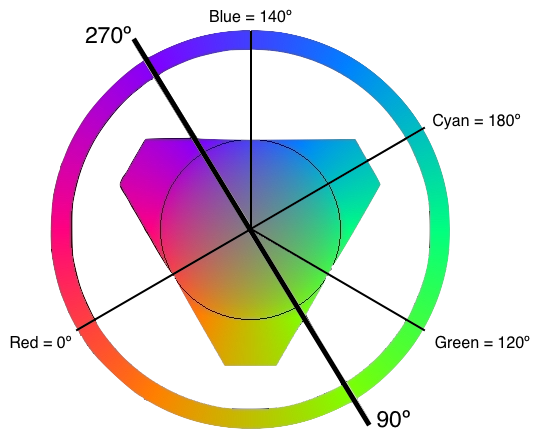
\includegraphics[width=0.5\textwidth]{images/HSV_hue.png}
  \caption[Example of HSV Hue Circle, with opposed hue values.]{Example of HSV Hue Circle, with opposed hue values. Depicted: Questions 3 and 4, with resulting hues $270º$ and $90º$.}
  \label{fig:hsvcircles_example}
\end{figure}
%
As referred before, there are some color blends that, due to the fact that primitives of the mixture are precisely opposed ($180º$) in the HSV hue circle, the blending in HSV Model could produce two different outputs.
This occurs if one mixes the colors obeying to a positive or negative rotation on the circle (as seen on figure \ref{fig:hsvcircles_example}). There are in this study three pairs of colors which blend onto two possible
colors: pair Red-Cyan (with possible outputs question three and four), pair Green-Magenta (questions ten and eleven) and pair Blue-Yellow (questions fifteen and sixteen). By placing these questions, we intended to
understand which side the user would tend to follow (or even if he follows one) when asked to indicate the blending-basis. The results for each question were already analyzed in the previous subsection, therefore we
present the essence of them in the following topics:
%
\begin{enumerate}
  \item \ul{Red \& Cyan Blend} - Analyzing answers for questions three and four, they produce fairly similar results: they are both a bit far from the expected colors ($\tilde{x}_{distance-3} = 0.0941$ and
  $\tilde{x}_{HSV-4} = 0.1162$), although the mean distance to the HSV precalculated blending for question three has a slightly lower value than question four. This could be also compared to question 12, which also
  produces \textbf{Lime-Green} like question three, but even when compared, question three still has the best results when generating this tone of green. This leads us to specifiy that, although the mean distances to the
  ideal HSV Color blend for this mixture, are not the lowest among all questions, \textbf{the users show a tendency to associate the blending of red and cyan to a result of lime-green, instead of shade of purple}. When comparing
  these results with online, we found that the later ones corroborate and prove this conclusion.
  %
  \item \ul{Green \& Magenta Blend} - Unlike the previous blend, the results bewteen these questions were quite different between each other concerning the distance to the expected colors: $\tilde{x}_{HSV-10} = 0.3$
  and $\tilde{x}_{HSV-11} = 0.0587$. However, the lower results associated with question eleven are due to the simple fact that \textbf{users indicated answers pairs which contained Red and Yellow}, which is the pair
  analyzed previously that also blended into orange; if the distance to the ideal answer pair for this question was measured, its mean value would be $\tilde{x}_{distanceC1-C2} = 0.645$, which is largely different from the
  expected colors. Therefore we can conclude that \textbf{it is hard for the users to blend green and magenta, to obtain either a blue or an orange shade}; we can also conclude that \textbf{the blending of red and yellow
  onto an orange color, is a strongly implemented color mixture, in mental models of our users}.
  %
  \item \ul{Blue \& Yellow Blend} - Evaluating the results obtained on question fifteen and sixteen, we obtain different results for both. Analyzing results of question fifteen, we know that the distance to the expected
  pair of colors it presents one of the lowest values among all results for HSV Color Model ($\tilde{x}_{HSV-15} = 0.09$, $\sigma_{HSV-15} = 0.03559$); however, when comparing the result-pairs given on this question, with
  the ones given on question nine (which presented the exact same shade of green, when asked for pair Green-Cyan), question fifteen still presents the results to generate this color.
  As it can be seen on Figure \ref{fig:labhsvregular_15}, the resulting blend in HSV Color Model tend to be close to the ideal HSV answer: despite being nearer to the top corner of the HSV Model Triangle, \textbf{we can still
  consider the answers to be a tone of green color}. Regarding the results from question 16, they present themselves to be one of the worst for this color model: the distance to the expected colors is $\tilde{x}_{HSV-16} = 0.2087$
  and the standard deviation for the distances of answers blended in HSV is $\sigma_{HSV-16} = 0.10378$. Since the presented color had a strong value of red component, users tended their answers to the red shade, while blending
  it with a purple or pink one, to indicate a mixture close to magenta. This indicates that \textbf{blending Blue and Yellow, in HSV Color Model, does not correspond to a red shade, but to a green one, according to
  the users' expectations}.
  %
  \begin{figure}[!htbp]
    \centering
    \begin{minipage}{0.48\textwidth}
      \centering
      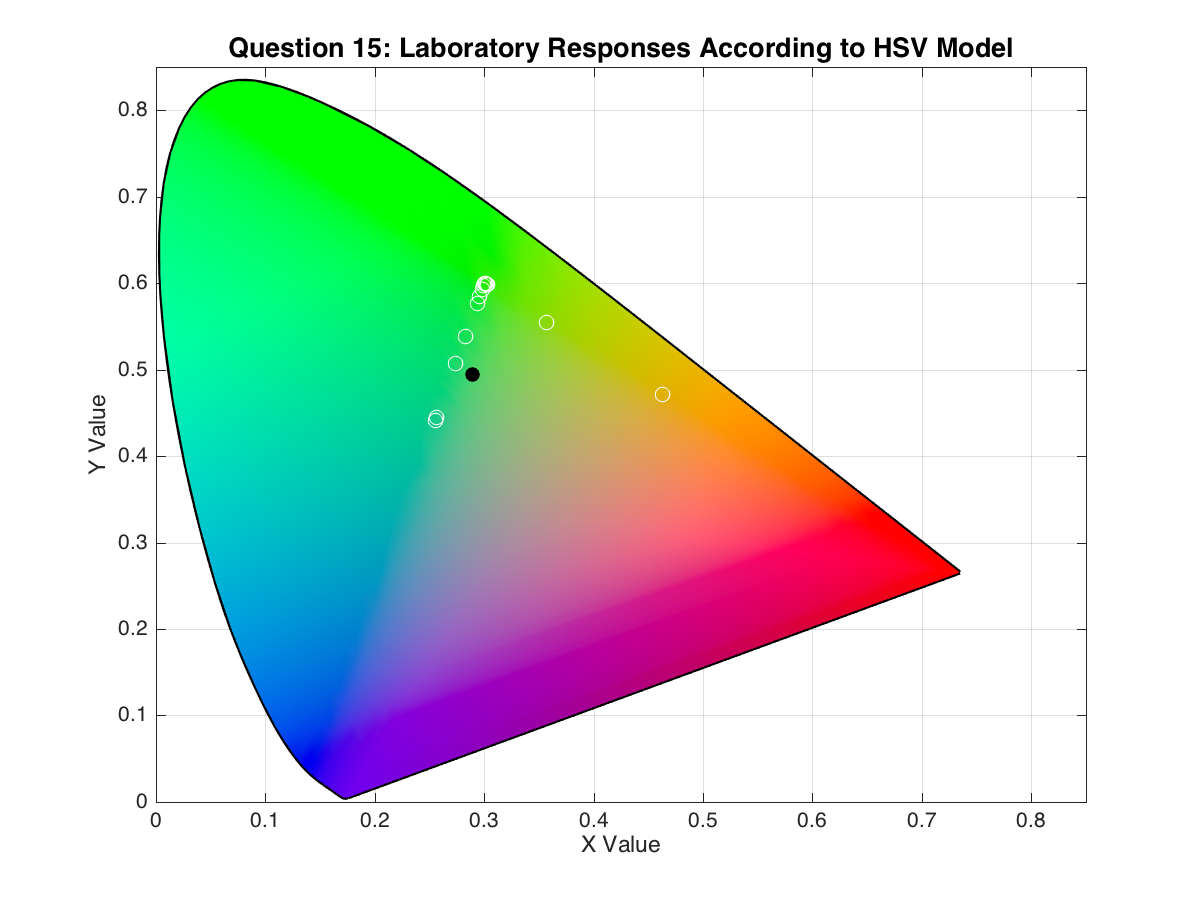
\includegraphics[width=\textwidth]{images/15_lab_HSVresponses.png}
      \caption[Laboratory Results: Answers for Question 15, from regular users, mixed in HSV Color Model.]{Laboratory Results: Answers for Question 15, from regular users, mixed in HSV Color Model.}
      \label{fig:labhsvregular_15}
    \end{minipage}\hfill
    \begin{minipage}{0.48\textwidth}
      \centering
      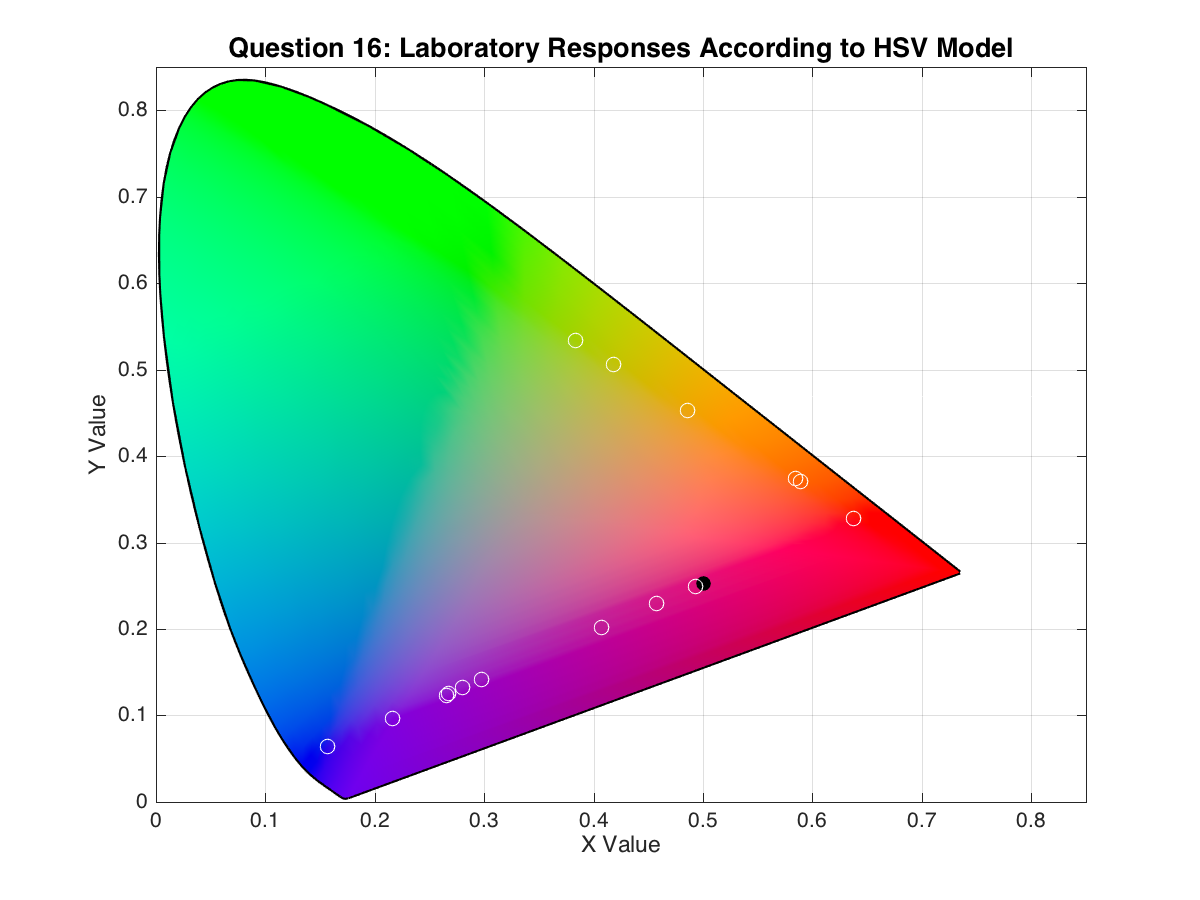
\includegraphics[width=\textwidth]{images/16_lab_HSVresponses.png}
      \caption[Laboratory Results: Answers for Question 16, from regular users, mixed in HSV Color Model.]{Laboratory Results: Answers for Question 16, from regular users, mixed in HSV Color Model.}
      \label{fig:labhsvregular_16}
    \end{minipage}
  \end{figure}
  %
\end{enumerate} \par
%
Another interesting example is Question ten and thirteen: they both present a shade of blue, which could be obtained by two strands, either Green and Magenta (Question ten) or Blue and Cyan (Question thirteen). Particularly, the
late question had a fairly simple expected pair (two shades of blue), but the users demonstrated some dispersion when aswering the question: moreover, the statistics prove it, by having a rather high standard deviation
($\tilde{x}_{HSV-10} = 0.3$, $\sigma_{HSV-10} = 0.15792$) when compared to the standard deviation of the whole model ($\sigma_{HSV} = 0.08$). These results are, thus, consistent with the know fact [\textbf{COLOCAR REF}] that
\textbf{human color perception is poorer in the blue region of the color spectrum, than in others}, \emph{e.g} the green zone, which produced the best results for this color model; these results are extensible to the purple region
of the spectrum, which is contiguous to the blue one. \par
%
The diagram of Figure \ref{fig:hsv_analysis} contains the three top and bottom-valued questions, disposed on top of an interval $[0 ; 0.5]$ of differences. Each question is mapped according to its mean value for distance to the ideal
HSV Color Model response, while is accompanied by the range of values which compose its answers. \par
%
\begin{figure}[!htbp]
  \centering
  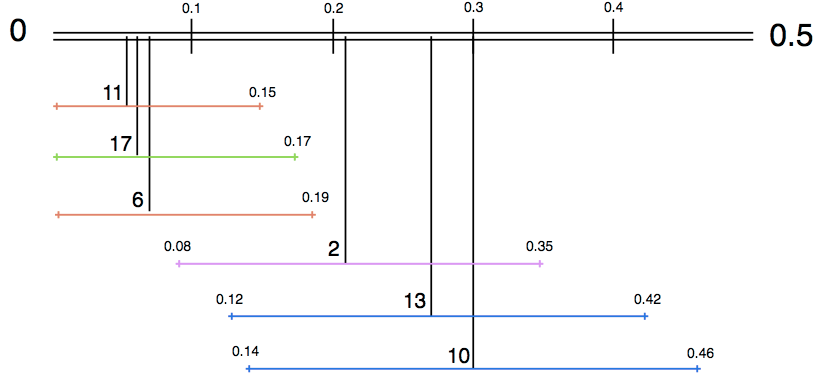
\includegraphics[width=0.9\textwidth]{images/hsv_questions_analysis.png}
  \caption[Best and Worst Questions, according to HSV Color Model.]{Best and Worst Questions, according to HSV Color Model.}
  \label{fig:hsv_analysis}
\end{figure}
%
%%%%%%%%%%%%%%%%%% LCh Analise %%%%%%%%%%%%%%%%%%
%
\paragraph{\ul{CIE-L*C*h* Color Model Blendings}} \par
\label{par:lchcolormodel}
%
In turn, the CIE-L*C*h* Color Model is the one which presents the worst results for most of the descriptive statistics present on Table \ref{table:colormodels_distances_labonline_statistics}: it has the highest
mean value on laboratory and online environment, and the highest standard deviation, range and variance exclusively on the online environment. These results are consistent with the individual questions' values, seen before this
section. \par
%
The three questions which have shorter distances are number six (given orange, expected red and yellow), number five (given a shade of red, expected red and magenta) and number two (given magenta, expected red
and blue). The mean values distances for this questions were $\tilde{x}_{6} = 0.1332$, $\tilde{x}_{5} = 0.15$ and $\tilde{x}_{2} = 0.1573$ which, contrary to the previous color model, are all values above $0.1$ (a quite
high value in the scale which results are presented), that could represent a significant change in the resultant color. \par
%
On the other hand, we consider that the questions which generate the worst results are number ten (given a shade of blue, expected green and magenta), number fourteen (given a shade of purple, expected blue and magenta) and number
fifteen (given a shade of green, expected blue and yellow), with correspondent mean values $\tilde{x}_{10} = 0.2557$, $\tilde{x}_{14} = 0.2995$ and $\tilde{x}_{15} = 0.3031$. Curiously, the standard deviations of distances (for the
laboratory environment) in this color model are fairly low when compared to the previous color model. \par
%
When comparing the results from the CIE-L*C*h* color model with other color models' results, we detect some statiscally significant differences with other models: performing a Wilcoxon Test ($p < 0.05$), we can infer that CIE-L*C*h* does
present statistically significant differences with HSV, CMYK, RGB and CIE-L*a*b* in the majority of questions (between 8 to 10 questions). The model which CIE-L*C*h* has most statistically significant differences with is CMYK, with eleven questions. \par
%
Question six presented again a constant top value for the mean value, on this model, which reinforces the theory that the \textbf{orange color is commonly used and mixed by the users}. On the other hand, question number
ten kept having one of the worst mean ($\tilde{x}_{10} = 0.2557$) and deviation ($\sigma_{10} = 0.1164$) values, strengthening the theory that \textbf{blue shades and tones will probably wild worst results, due to the fact
that it is the color which human have less descriptive power}. \par
%
\begin{figure}[!htbp]
  \centering
  \begin{minipage}{0.48\textwidth}
    \centering
    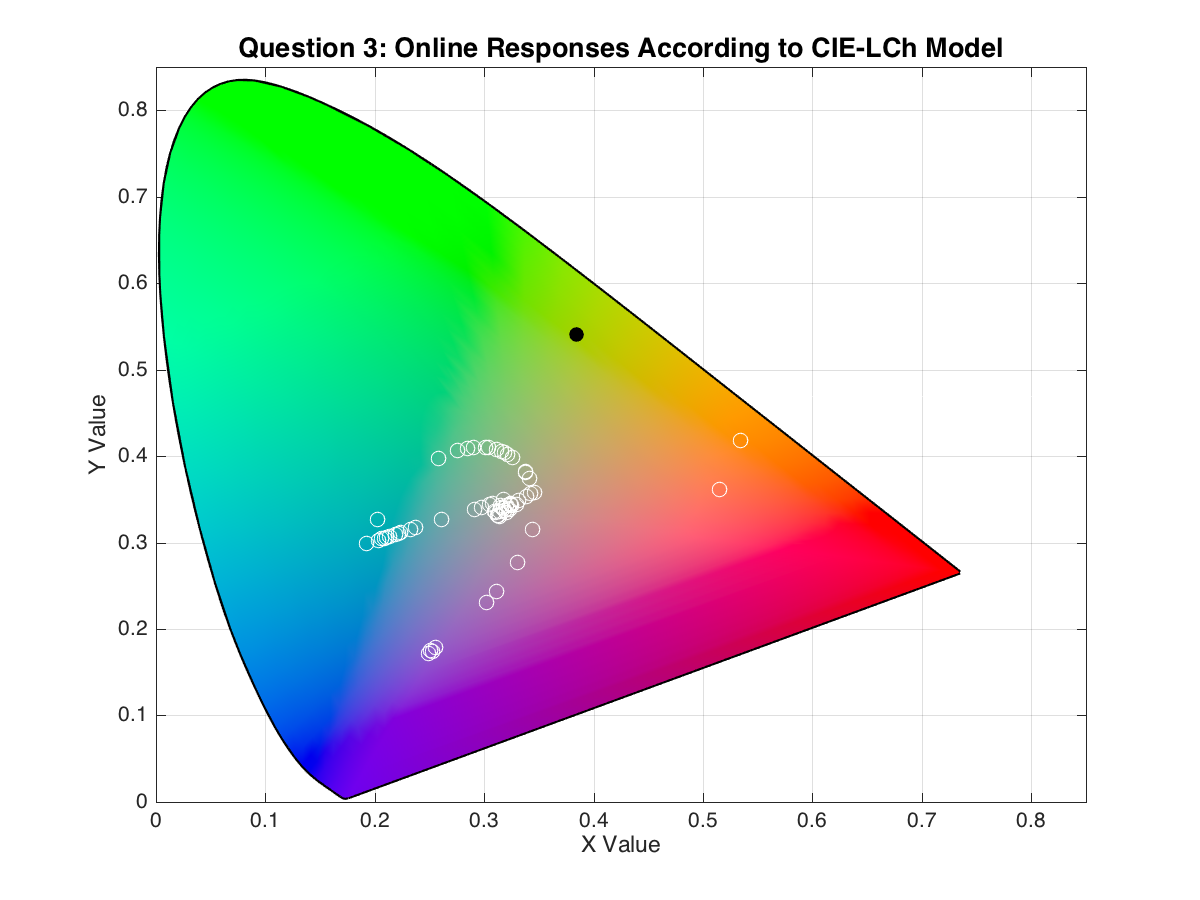
\includegraphics[width=\textwidth]{images/3_online_LChresponses.png}
    \caption[Online Results: Answers for Question 3, from regular users, mixed in CIE-L*C*h* Color Model.]{Online Results: Answers for Question 3, from regular users, mixed in CIE-L*C*h* Color Model.}
    \label{fig:onlinelchregular_3}
  \end{minipage}\hfill
  \begin{minipage}{0.48\textwidth}
    \centering
    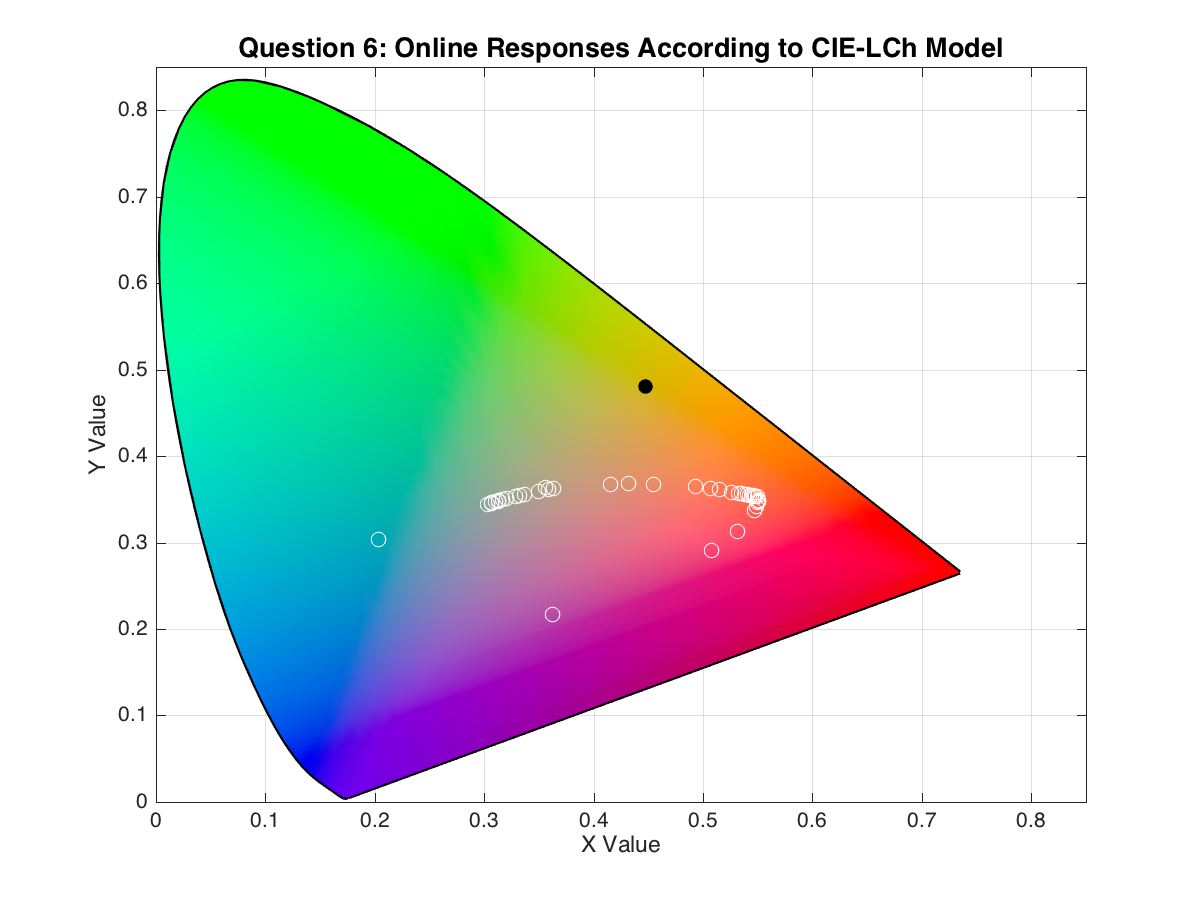
\includegraphics[width=\textwidth]{images/6_online_LChresponses.png}
    \caption[Online Results: Answers for Question 6, from regular users, mixed in CIE-L*C*h* Color Model.]{Online Results: Answers for Question 6, from regular users, mixed in CIE-L*C*h* Color Model.}
    \label{fig:onlinelchregular_6}
  \end{minipage}
\end{figure}
%
The question which revealed one of the lowest standard deviation value (meaning less osccilation of results), relating the online environment, was question three ($\sigma_{3} = 0.05855$): this question help us
illustrate the difference between each of the descriptive statistics, since it has one of the highest mean value of distances ($\tilde{x}_{17} = 0.23$) and, at the same time, lowest standard deviation. This could
portray a scenario in which the users agreed on a quite distant answer. This question is illustrated in Figure \ref{fig:onlinelchregular_3}. \par
%
The question which has the lowest mean value of distances was question six ($\sigma_{LCh-6} = 0.1332$), and it is represented on Figure \ref{fig:onlinelchregular_6}. Nonethless, we can observe that \textbf{these
questions have all answers pairs which, when blended according to CIE-L*C*h*, generate results that are farther apart from the ideal answer of each question}, therefore concluding that \textbf{CIE-L*C*h* is not
the color model which hatches the best results when blending colors, according to users' expectations}. \par
%
The diagram of Figure \ref{fig:lch_analysis} contains the three top and bottom-valued questions, disposed on top of an interval $[0 ; 0.5]$ of differences. Each question is mapped according to its mean value for
distance to the ideal CIE-L*C*h* Color Model response, while is accompanied by the range of values which compose its answers. \par
%
\begin{figure}[!htbp]
  \centering
  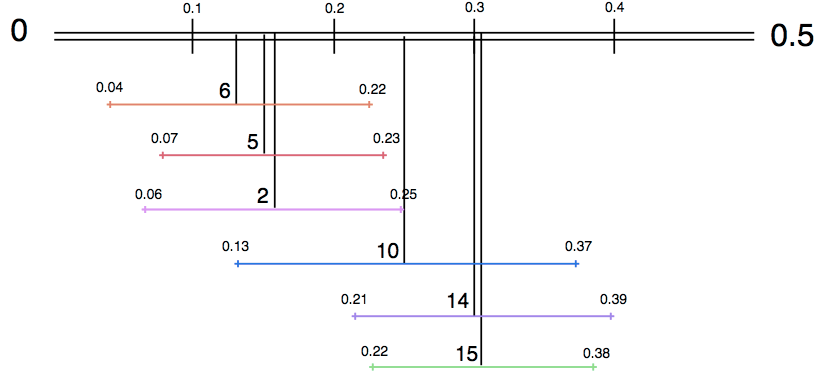
\includegraphics[width=0.9\textwidth]{images/lch_questions_analysis.png}
  \caption[Best and Worst Questions, according to CIE-L*C*h* Color Model.]{Best and Worst Questions, according to CIE-L*C*h* Color Model.}
  \label{fig:lch_analysis}
\end{figure}
%
%%%%%%%%%%%%%%%%%% CMYK Analise %%%%%%%%%%%%%%%%%%
%
\paragraph{\ul{CMYK Color Model Blendings}}
\label{par:cmykcolormodel}
%
The CMYK Color Model is, by far, the one which presents the best results for most of the descriptive statistics present on Table \ref{table:colormodels_distances_labonline_statistics}, being authenticated by the
results from the online environment: it has the lowest mean value of distances ($\tilde{x}_{lab} = 0.10$, $\tilde{x}_{online} = 0.09$), lowest standard deviation ($\sigma_{lab} = 0.04$, $\sigma_{online} = 0.04$),
the lowest range of values ($range_{lab} = 0.14$, $range_{online} = 0.11$) and, finally, the lowest variance value ($\sigma^2_{lab} = 0.001$, $\sigma^2_{online} = 0.001$). \par
%
The three questions which have shorter distances are number seventeen (given a green, expected cyan and blue), number six (given orange, expected red and yellow) and number fifteen (given a shade of green, expected blue
and yellow). The mean values distances for this questions were $\tilde{x}_{17} = 0.0452$, $\tilde{x}_{6} = 0.0577$ and $\tilde{x}_{15} = 0.0625$ which, contrary to the previous color model, are all values \ul{below $0.1$},
that does not represent a significant change in the resultant color. \par
%
On the other hand, we consider that the questions which generate the worst results are number ten (given a shade of blue, expected green and magenta) and twelve (given a tone of green, expected green and yellow), number five
(given a shade of red, expected red and magenta) and number thirteen (given a shade of blue, expected blue and cyan), with correspondent mean values $\tilde{x}_{10-12} = 0.1314$, $\tilde{x}_{5} = 0.1322$ and
$\tilde{x}_{13} = 0.1875$. Comparing them with the CIE-L*C*h* Color Model, we can easily observe that these values are very low when compared with the later's worst results. \par
%
Question six keeps presenting a constant top value for the mean value, on this model, while question number ten and thirteen (both presented blue shades) kept having the worst mean and deviation values ($\tilde{x}_{13} = 0.1875$,
$\sigma_{13} = 0.13097$), strengthening the theories aforementioned. \par
%
When comparing the results from the CMYK color model with other color models' results, we detect some statiscally significant differences with other models: performing a Wilcoxon Test ($p < 0.05$), we can infer that CMYK does
present statistically significant differences with HSV, CIE-L*C*h*, RGB and CIE-L*a*b* in the majority of questions. The model which CMYK has most statistically significant differences with is RGB, with thirteen questions. \par
%
Question seventeen presented consistently another low value: along with question three and fifteen, these presented different \ul{shades of green} and all had yielded favorable results. Having this in mind, this may lead us to
form another conclusion: \textbf{questions which presented shades of green color may produce better results, according to users' expectactions}. This is coherent with the fact that \textbf{humans have more descriptive power
in the green zone of the spectrum, due to the amount of cones which exist in the human eye}. \par
%
As it was explained before in the theoretical background, this color model is mainly a subtractive one, meaning it will naturally darken the colors when they are blended; the questions which yielded \textbf{better results are majorly
related to primitives of the CMYK color model}. This success could be related to the fact that \textbf{people tend to formulate mental models of color based on ink mixing in childhood} \cite{Gossett2004}, mostly associating it to
\gls{RYB} and CMYK Color Models without even knowing it. \par
%
\begin{figure}[!htbp]
  \centering
  \begin{minipage}{0.48\textwidth}
    \centering
    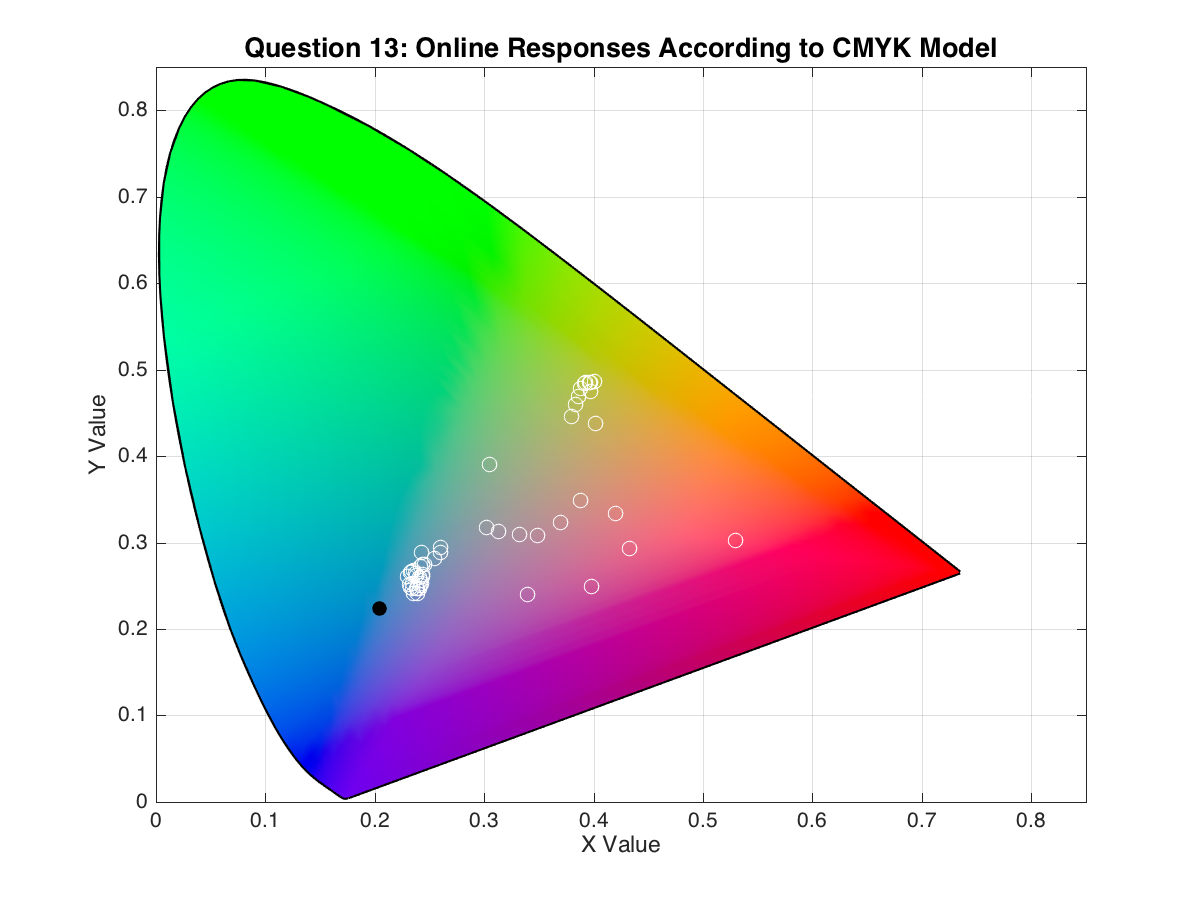
\includegraphics[width=\textwidth]{images/13_online_CMYKresponses.png}
    \caption[Online Results: Answers for Question 13, from regular users, mixed in CMYK Color Model.]{Online Results: Answers for Question 13, from regular users, mixed in CMYK Color Model.}
    \label{fig:onlinecmykregular_13}
  \end{minipage}\hfill
  \begin{minipage}{0.48\textwidth}
    \centering
    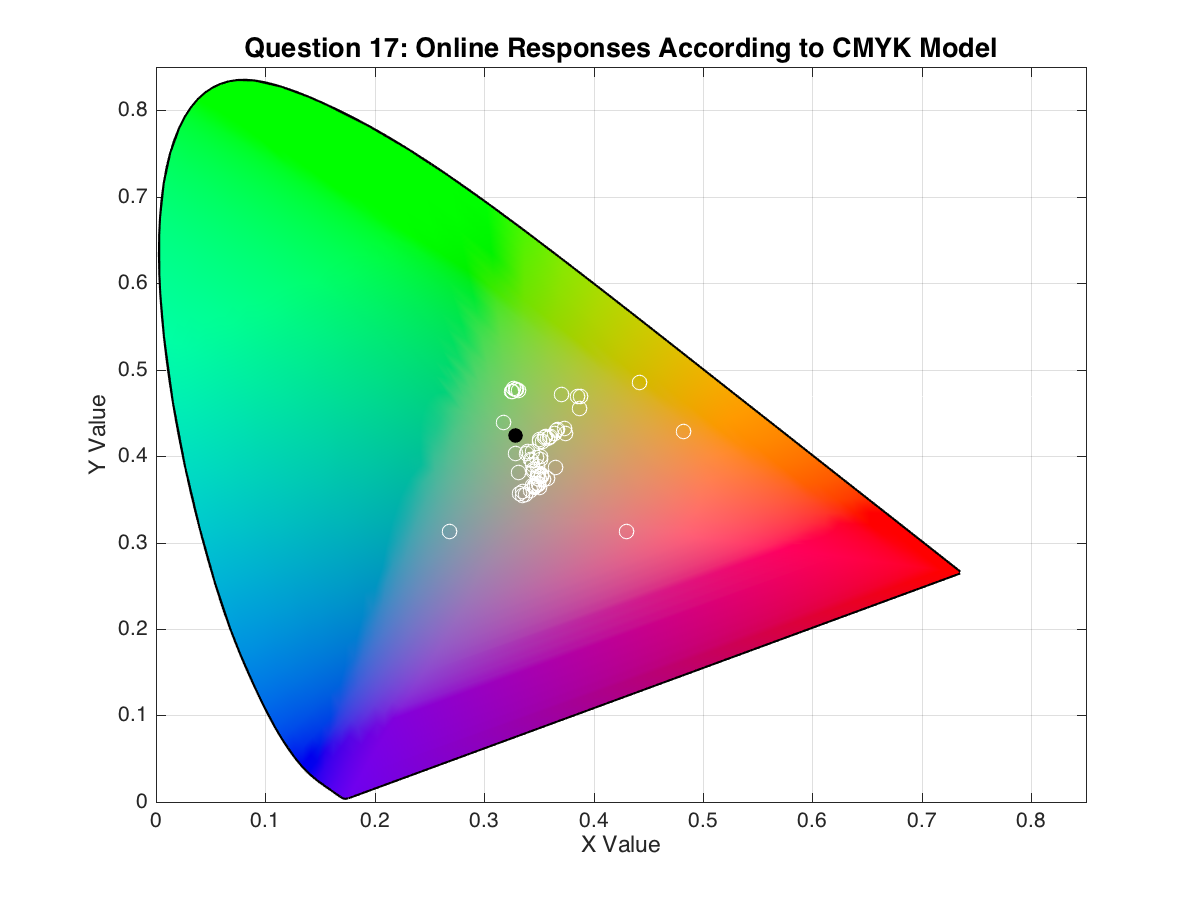
\includegraphics[width=\textwidth]{images/17_online_CMYKresponses.png}
    \caption[Online Results: Answers for Question 17, from regular users, mixed in CMYK Color Model.]{Online Results: Answers for Question 17, from regular users, mixed in CMYK Color Model.}
    \label{fig:onlinecmykregular_17}
  \end{minipage}
\end{figure}
%
These results indicate that \textbf{CMYK is a highly compatible color model with the users expectations}, as this model presents statistics which prove that CMYK had smaller distances to ideal answers and lower deviation of answers.
Figure \ref{fig:onlinecmykregular_13} represents the results of Question 13, which had wider distances to the pre-calculated CMYK blend, and Figure \ref{fig:onlinecmykregular_17} show the results for Question 17, the question with closer
distances. The diagram of Figure \ref{fig:cmyk_analysis} contains the three top and bottom-valued questions, disposed on top of an interval $[0 ; 0.5]$ of differences. Each question is mapped according to its mean value for
distance to the ideal CMYK Color Model response, while is accompanied by the range of values which compose its answers. \par
%
\begin{figure}[!htbp]
  \centering
  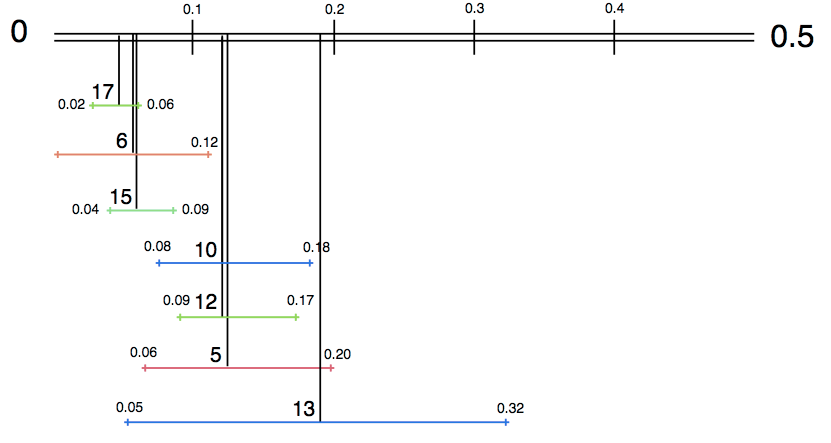
\includegraphics[width=0.9\textwidth]{images/cmyk_questions_analysis.png}
  \caption[Best and Worst Questions, according to CMYK Color Model.]{Best and Worst Questions, according to CMYK Color Model.}
  \label{fig:cmyk_analysis}
\end{figure}
%
%%%%%%%%%%%%%%%%%% RGB Analise %%%%%%%%%%%%%%%%%%
%
\paragraph{\ul{RGB Color Model Blendings}}
\label{subsubsec:rgbcolormodel}
%
This color model, as covered before, is complementary to the CMYK color model. Feedback collected from the users was such that, sometimes, the users which knew how to blend in subtractive color models,
tended to be confused and tried to mix additive color models, also. Based on the results collectd from the laboratory users, we can tell that the results from this color model are quite similar to CMYK results: the descriptive statistics present
on Table \ref{table:colormodels_distances_labonline_statistics}, authenticated by the results from the online environment, prove RGB has one of the lowest mean value of distances ($\tilde{x}_{lab} = 0.14$, $\tilde{x}_{online} = 0.12$) and one of
the lowest standard deviations ($\sigma_{lab} = 0.05$, $\sigma_{online} = 0.04$ equal to $\sigma_{CMYK-online}$). \par
%
The three questions which have shorter distances are number number six (given orange, expected red and yellow), number nine (given a shade of green, expected green and cyan) and seventeen (given a green, expected cyan and blue). The mean values
distances for this questions were $\tilde{x}_{6} = 0.0777$, $\tilde{x}_{9} = 0.1005$ and $\tilde{x}_{17} = 0.1030$. \par
%
On its turn, we consider that the questions which generate the worst results are number two (given magenta, expected red and blue), number ten (given a shade of blue, expected green and magenta) and, again, number thirteen (given a shade of blue,
expected blue and cyan), with correspondent mean values $\tilde{x}_{2} = 0.1660$, $\tilde{x}_{10} = 0.2107$ and $\tilde{x}_{13} = 0.2450$.
Comparing them with the CIE-L*C*h* Color Model, we can observe these values are likely to be similar when compared with the later's worst results, but a little high when compared with CMYK results. \textbf{The colors orange and green continue to
present the best values, while the blue shades are the lowest}. \par
%
When comparing the results from the RGB color model, the majority of users did reveal lack of knowledge in mixing the colors according to an additive color model, as they tended to mix colors according to the CMYK color model. However, this color
model has a high degree of compatibility with every other model, excepting CMYK: performing a Wilcoxon Test ($p < 0.05$), we can infer that RGB does not present statistically significant differences with HSV, CIE-L*a*b* and with CIE-L*C*h* in the
majority of questions (ten questions), while presenting statistically significant differences with CMYK in thirteen questions. \par
%
Relating to the fact that people either tend to blend colors in an additive or subtractive way, we can compare the results from this color model with CMYK model and state that \textbf{users tend to formulate subtractive mental models of color
blending}. However, \textbf{there is room for further investigation, to fully understand if users are influenced by additive color models (\emph{e.g.} RGB) or subtractive ones (\emph{e.g.} CMYK)}. \par
%
\begin{figure}[!htbp]
  \centering
  \begin{minipage}{0.48\textwidth}
    \centering
    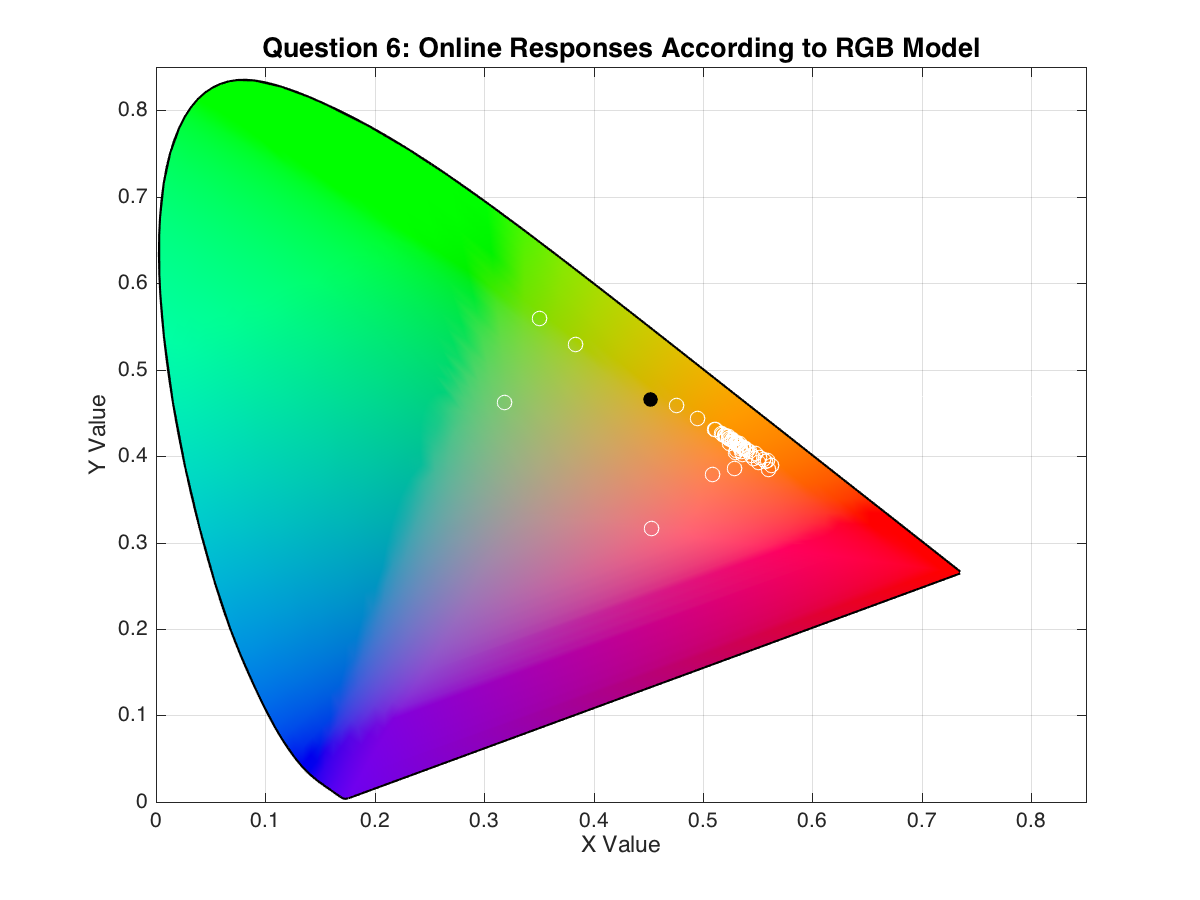
\includegraphics[width=\textwidth]{images/6_online_RGBresponses.png}
    \caption[Online Results: Answers for Question 6, from regular users, mixed in RGB Color Model.]{Online Results: Answers for Question 6, from regular users, mixed in RGB Color Model.}
    \label{fig:onlinergbregular_6}
  \end{minipage}\hfill
  \begin{minipage}{0.48\textwidth}
    \centering
    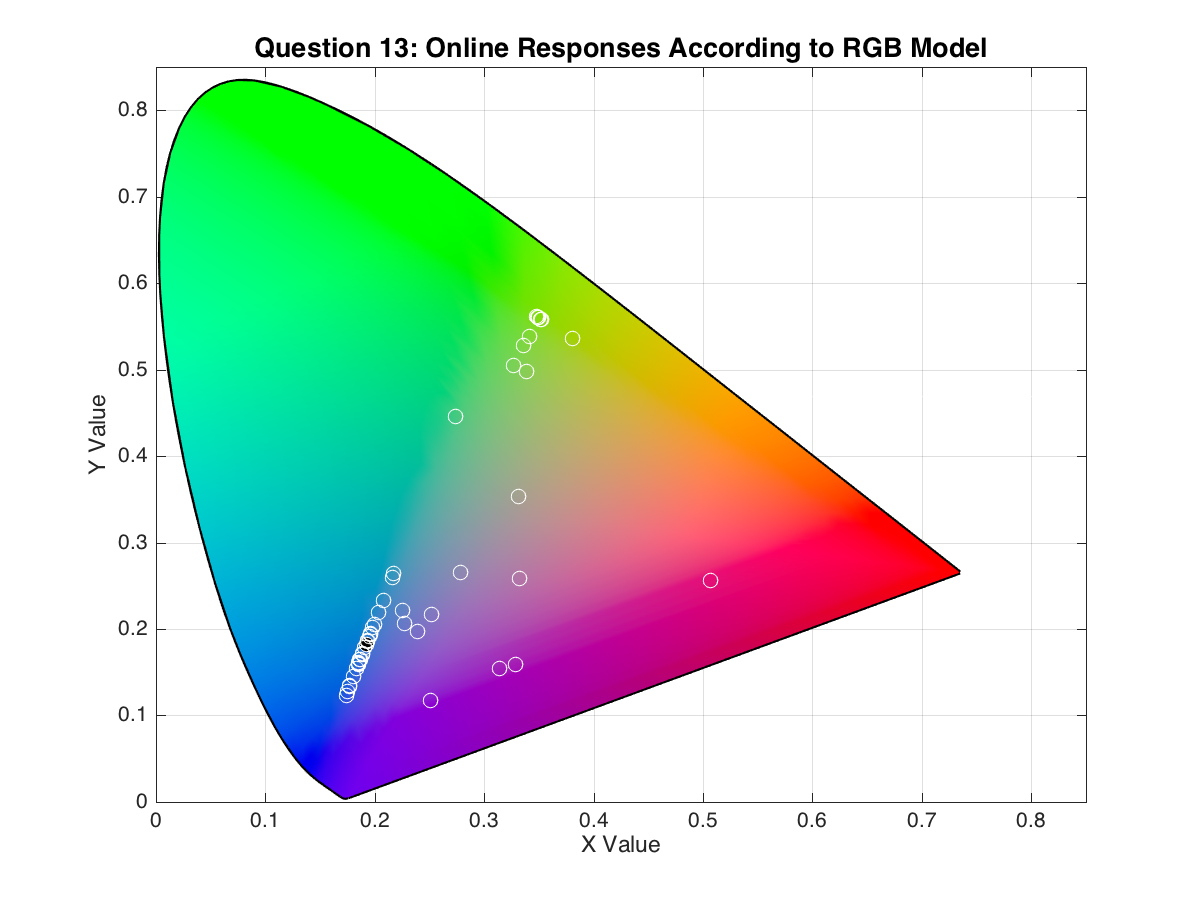
\includegraphics[width=\textwidth]{images/13_online_RGBresponses.png}
    \caption[Online Results: Answers for Question 13, from regular users, mixed in RGB Color Model.]{Online Results: Answers for Question 13, from regular users, mixed in RGB Color Model.}
    \label{fig:onlinergbregular_13}
  \end{minipage}
\end{figure}
%
Figure \ref{fig:onlinergbregular_6} represents the results of Question 6, which had the shortest distances to the pre-calculated RGB blend, and Figure \ref{fig:onlinergbregular_13} show the results for Question 13, the question with wider
distances. The diagram of Figure \ref{fig:rgb_analysis} contains the three top and bottom-valued questions, disposed on top of an interval $[0 ; 0.5]$ of differences. \par
%
\begin{figure}[!htbp]
  \centering
  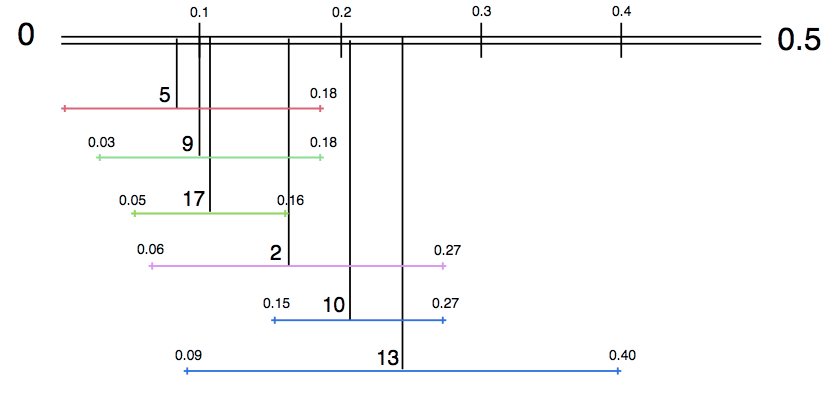
\includegraphics[width=0.9\textwidth]{images/rgb_questions_analysis.png}
  \caption[Best and Worst Questions, according RGB Color Model.]{Best and Worst Questions, according to RGB Color Model.}
  \label{fig:rgb_analysis}
\end{figure}
%
%%%%%%%%%%%%%%%%%% Lab Analise %%%%%%%%%%%%%%%%%%
%
\paragraph{\ul{CIE-L*a*b* Color Model Blendings}} \par
\label{par:lchcolormodel}
%
This color model has results very similar to CMYK and RGB, since its descriptive statistics have comparable values to this model. \par
%
The three questions which have shorter distances are number number six (given orange, expected red and yellow), seventeen (given a green, expected cyan and blue) and number nine (given a shade
of green, expected green and cyan), which are exactly the same as before. The mean values distances for this questions were $\tilde{x}_{6} = 0.0509$, $\tilde{x}_{17} = 0.1130$ and $\tilde{x}_{9} = 0.1142$. \par
%
Considerint the questions which generate the worst results are number twelve (given a tone of green, expected green and yellow), number ten (given a shade of blue, expected green and magenta) and number thirteen
(given a shade of blue, expected blue and cyan), with correspondent mean values $\tilde{x}_{12} = 0.1743$, $\tilde{x}_{10} = 0.2107$ and $\tilde{x}_{13} = 0.2450$. Comparing them with the CIE-L*C*h* Color Model
(which is currently the worst-valued color model), we can check that these values are (similar to RGB and HSV) nearer to the later's worst results, but still high when compared with CMYK results (so far, the
best-valued color model). \textbf{The colors orange and green proved, once again, that they are capable of producing the best values, while the blue shades provided the lowest again}. \par
%
When comparing the results from the CIE-L*a*b* color model, we detected that this model has significant differences with all other color models: performing a Wilcoxon Test ($p < 0.05$), we can infer that
CIE-L*a*b* does present statistically significant differences with HSV, CMYK and with CIE-L*C*h* in only nine questions, while presenting no statistically significant differences with RGB
in ten questions. \par
%
Since the CIE-L*a*b* conveys the entire set of perceived by the human eye, it \textbf{explains why the results associated with this color model are so close to others which yield the best results}.
%
\begin{figure}[!htbp]
  \centering
  \begin{minipage}{0.48\textwidth}
    \centering
    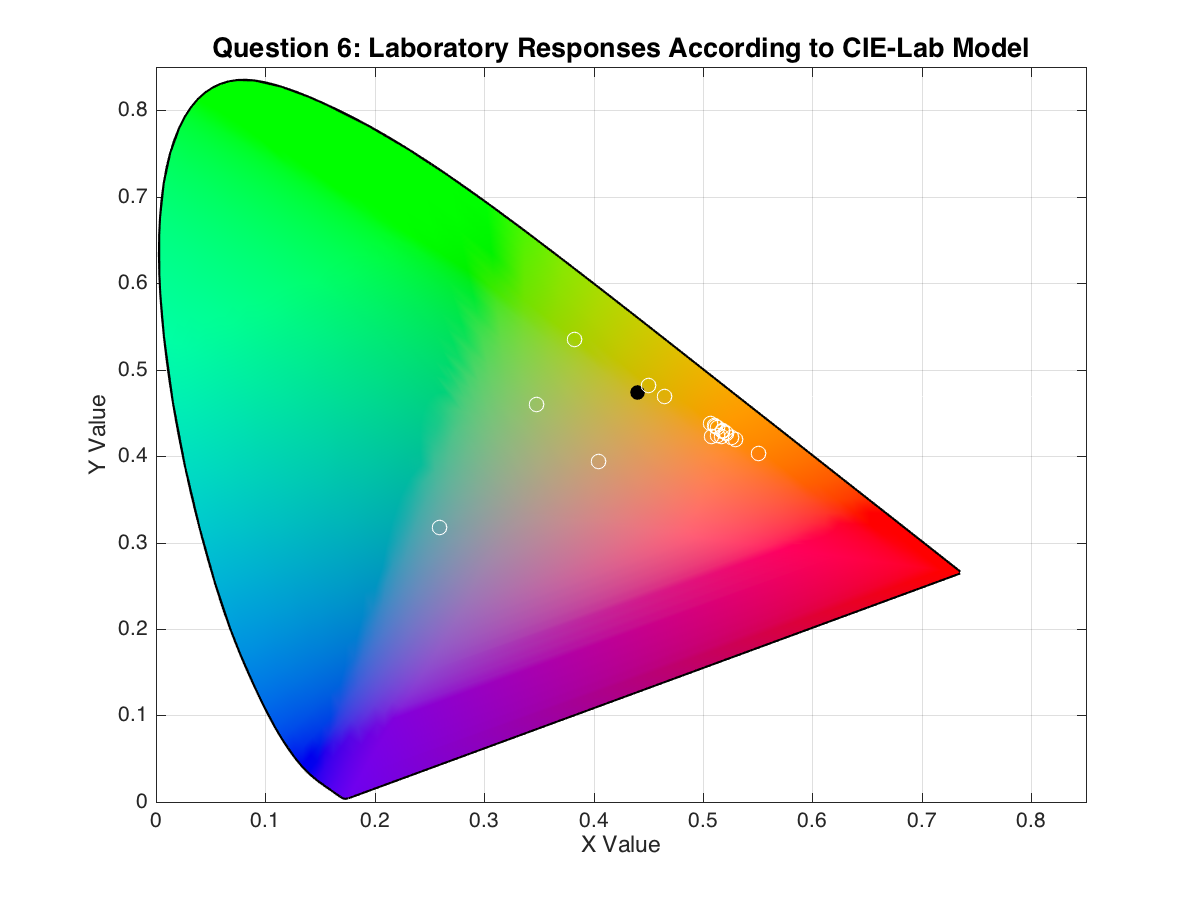
\includegraphics[width=\textwidth]{images/6_lab_Labresponses.png}
    \caption[Laboratory Results: Answers for Question 6, from regular users, mixed in CIE-L*a*b* Color Model.]{Laboratory Results: Answers for Question 6, from regular users, mixed in CIE-L*a*b* Color Model.}
    \label{fig:lablabregular_6}
  \end{minipage}\hfill
  \begin{minipage}{0.48\textwidth}
    \centering
    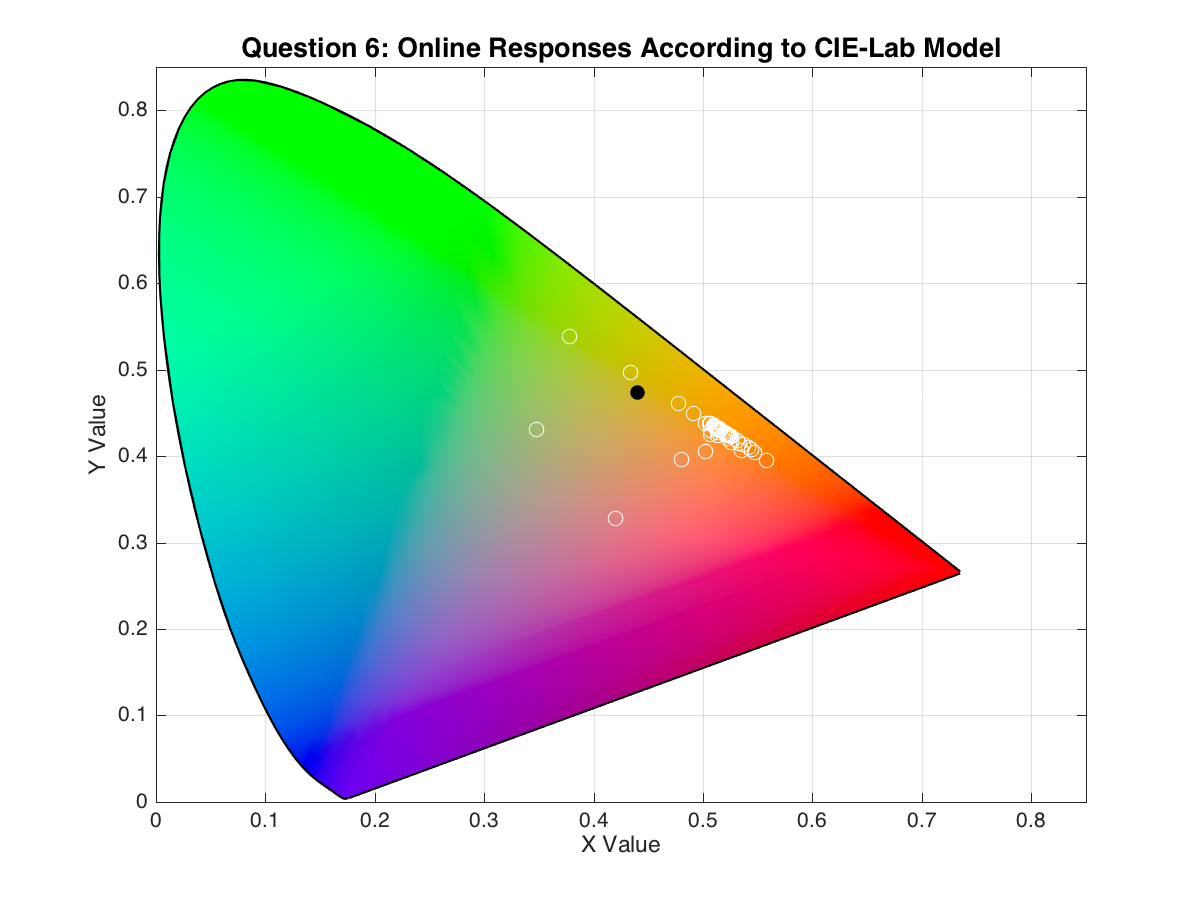
\includegraphics[width=\textwidth]{images/6_online_Labresponses.png}
    \caption[Online Results: Answers for Question 6, from regular users, mixed in CIE-L*a*b* Color Model.]{Laboratory Results: Answers for Question 6, from regular users, mixed in CIE-L*a*b* Color Model.}
    \label{fig:onlinelabregular_6}
  \end{minipage}
\end{figure}
%
Figure \ref{fig:lablabregular_6} represents the laboratory results of Question 6, which not only had the best mean value to the pre-calculated RGB blend, but also its best mean value across all color models,
and Figure \ref{fig:onlinelabregular_6} shows the results for the same question, but the online results which confirm the laboratory ones. The diagram of Figure \ref{fig:lab_analysis} contains the three top and bottom-valued questions, disposed on top of an interval $[0 ; 0.5]$ of differences. \par
%
\begin{figure}[!htbp]
  \centering
  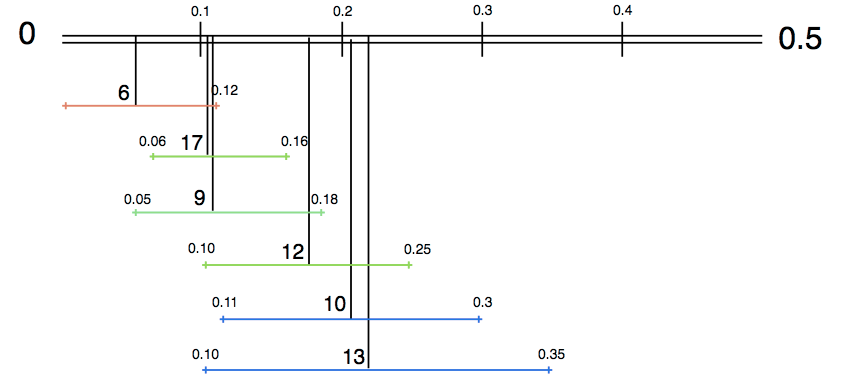
\includegraphics[width=0.9\textwidth]{images/lab_questions_analysis.png}
  \caption[Best and Worst Questions, according to CIE-L*a*b* Color Model.]{Best and Worst Questions, according to CIE-L*a*b* Color Model.}
  \label{fig:lab_analysis}
\end{figure}
%
\subsubsection{Color Blending Expectation}
\label{subsubsec:colorblending_exp}
%
Besides asking our users to indicate us the two primitives which composed a color blending of two colors, we intended to go further: \textbf{comprehend if more than detecting two colors of a mixture, a user
is capable of mentally blend two given colors and indicate us its results}. \par
%
Therefore, we reverted the previously analyzed seventeen questions, giving the two primitives of the blending to the user, offering at the same time a color slider which contained discretized pre-calculated
values (which were nothing more than all the results of all questions, blended accordingly to all color models). Contrary to what was done previously, \textbf{we did not blend the answer given by the user,
since the colors presented were already blended}, missing only to calculate the distance of answers to the ideal ones: the results for these questions are expressed on Table \ref{table:expectation_distances_labonline},
with cells shaded in green which represent the best value for each one of questions. \par
%
\begin{table}[!htbp]
  \resizebox{\textwidth}{!} {
  \begin{tabular}{@{}cccccclccccclcccc@{}}
    \toprule
                                     & \multicolumn{2}{c}{Presented Colors}                        & \multicolumn{2}{c}{}                                                                                                  & \multicolumn{6}{c}{Laboratory Environment}                                                                                                                                                                                                                                                                     & \multicolumn{6}{c}{Online Environment}                                                                                                                                                                                                                                                                         \\ \cmidrule(lr){2-3} \cmidrule(l){6-17}
    \multirow{-2}{*}{Question ID}    & C1                           & C2                           & \multicolumn{2}{c}{\multirow{-2}{*}{Expected Color}}                                                                  & \multicolumn{2}{c}{HSV}                                    & CIE-L*C*h*                                                 & CMYK                                                       & RGB                                                        & CIE-L*a*b*                                                 & \multicolumn{2}{c}{HSV}                                    & CIE-L*C*h*                                                 & CMYK                                                       & RGB                                                        & CIE-L*a*b*                                                 \\ \midrule
    \multicolumn{1}{c|}{Question 18} & \multicolumn{1}{c|}{Red}     & \multicolumn{1}{c|}{Green}   & \multicolumn{2}{c||}{\cellcolor[HTML]{FFFF00}(77, 93, 14)}                                                             & \multicolumn{2}{c|}{0.14}                                  & \multicolumn{1}{c|}{0.14}                                  & \multicolumn{1}{c|}{\cellcolor[HTML]{32CB00}\textbf{0.11}} & \multicolumn{1}{c|}{0.15}                                  & \multicolumn{1}{c||}{0.14}                                  & \multicolumn{2}{c|}{\cellcolor[HTML]{FFFFFF}0.12}          & \multicolumn{1}{c|}{\cellcolor[HTML]{FFFFFF}0.12}          & \multicolumn{1}{c|}{\cellcolor[HTML]{32CB00}\textbf{0.08}} & \multicolumn{1}{c|}{\cellcolor[HTML]{FFFFFF}0.12}          & \multicolumn{1}{c|}{0.11}                                  \\ \midrule
    \multicolumn{1}{c|}{Question 19} & \multicolumn{1}{c|}{Red}     & \multicolumn{1}{c|}{Blue}    & \multicolumn{2}{c||}{\cellcolor[HTML]{FF00FF}(59, 28, 97)}                                                             & \multicolumn{2}{c|}{\cellcolor[HTML]{32CB00}\textbf{0.16}} & \multicolumn{1}{c|}{0.23}                                  & \multicolumn{1}{c|}{0.17}                                  & \multicolumn{1}{c|}{\cellcolor[HTML]{32CB00}\textbf{0.16}} & \multicolumn{1}{c||}{0.19}                                  & \multicolumn{2}{c|}{\cellcolor[HTML]{32CB00}\textbf{0.13}} & \multicolumn{1}{c|}{0.24}                                  & \multicolumn{1}{c|}{0.19}                                  & \multicolumn{1}{c|}{0.14}                                  & \multicolumn{1}{c|}{0.19}                                  \\ \midrule
    \multicolumn{1}{c|}{Question 20} & \multicolumn{1}{c|}{Green}   & \multicolumn{1}{c|}{Blue}    & \multicolumn{2}{c||}{\cellcolor[HTML]{00FFFF}(54, 79, 107)}                                                            & \multicolumn{2}{c|}{0.13}                                  & \multicolumn{1}{c|}{0.17}                                  & \multicolumn{1}{c|}{0.14}                                  & \multicolumn{1}{c|}{0.13}                                  & \multicolumn{1}{c||}{\cellcolor[HTML]{32CB00}\textbf{0.11}} & \multicolumn{2}{c|}{0.12}                                  & \multicolumn{1}{c|}{0.17}                                  & \multicolumn{1}{c|}{0.13}                                  & \multicolumn{1}{c|}{0.12}                                  & \multicolumn{1}{c|}{\cellcolor[HTML]{32CB00}\textbf{0.10}} \\ \midrule
    \multicolumn{1}{c|}{Question 21} & \multicolumn{1}{c|}{Red}     & \multicolumn{1}{c|}{Cyan}    & \multicolumn{1}{c||}{\cellcolor[HTML]{80FF00}(45, 76, 12)} & \multicolumn{1}{c||}{\cellcolor[HTML]{7F00FF}(27, 12, 95)} & \multicolumn{1}{c|}{0.28}    & \multicolumn{1}{l|}{0.23}   & \multicolumn{1}{c|}{0.26}                                  & \multicolumn{1}{c|}{0.13}                                  & \multicolumn{1}{c|}{\cellcolor[HTML]{32CB00}\textbf{0.12}} & \multicolumn{1}{c||}{0.17}                                  & \multicolumn{1}{c|}{0.29}    & \multicolumn{1}{l|}{0.23}   & \multicolumn{1}{c|}{0.26}                                  & \multicolumn{1}{c|}{0.13}                                  & \multicolumn{1}{c|}{\cellcolor[HTML]{32CB00}\textbf{0.12}} & \multicolumn{1}{c|}{0.16}                                  \\ \midrule
    \multicolumn{1}{c|}{Question 22} & \multicolumn{1}{c|}{Red}     & \multicolumn{1}{c|}{Magenta} & \multicolumn{2}{c||}{\cellcolor[HTML]{FF0080}(45, 23, 22)}                                                             & \multicolumn{2}{c|}{\cellcolor[HTML]{32CB00}\textbf{0.18}} & \multicolumn{1}{c|}{0.20}                                  & \multicolumn{1}{c|}{0.25}                                  & \multicolumn{1}{c|}{0.21}                                  & \multicolumn{1}{c||}{0.20}                                  & \multicolumn{2}{c|}{\cellcolor[HTML]{32CB00}\textbf{0.14}} & \multicolumn{1}{c|}{0.16}                                  & \multicolumn{1}{c|}{0.20}                                  & \multicolumn{1}{c|}{0.17}                                  & \multicolumn{1}{c|}{0.16}                                  \\ \midrule
    \multicolumn{1}{c|}{Question 23} & \multicolumn{1}{c|}{Red}     & \multicolumn{1}{c|}{Yellow}  & \multicolumn{2}{c||}{\cellcolor[HTML]{FF8000}(49, 37, 5)}                                                              & \multicolumn{2}{c|}{\cellcolor[HTML]{32CB00}\textbf{0.16}} & \multicolumn{1}{c|}{\cellcolor[HTML]{32CB00}\textbf{0.16}} & \multicolumn{1}{c|}{\cellcolor[HTML]{32CB00}\textbf{0.16}} & \multicolumn{1}{c|}{0.18}                                  & \multicolumn{1}{c||}{\cellcolor[HTML]{32CB00}\textbf{0.16}} & \multicolumn{2}{c|}{0.09}                                  & \multicolumn{1}{c|}{\cellcolor[HTML]{32CB00}\textbf{0.08}} & \multicolumn{1}{c|}{\cellcolor[HTML]{32CB00}\textbf{0.08}} & \multicolumn{1}{c|}{0.10}                                  & \multicolumn{1}{c|}{\cellcolor[HTML]{32CB00}\textbf{0.08}} \\ \midrule
    \multicolumn{1}{c|}{Question 24} & \multicolumn{1}{c|}{Cyan}    & \multicolumn{1}{c|}{Magenta} & \multicolumn{2}{c||}{\cellcolor[HTML]{0000FF}(18, 7, 95)}                                                              & \multicolumn{2}{c|}{0.27}                                  & \multicolumn{1}{c|}{0.12}                                  & \multicolumn{1}{c|}{\cellcolor[HTML]{32CB00}\textbf{0.08}} & \multicolumn{1}{c|}{0.12}                                  & \multicolumn{1}{c||}{\cellcolor[HTML]{32CB00}\textbf{0.08}} & \multicolumn{2}{c|}{0.28}                                  & \multicolumn{1}{c|}{0.11}                                  & \multicolumn{1}{c|}{\cellcolor[HTML]{32CB00}\textbf{0.09}} & \multicolumn{1}{c|}{0.13}                                  & \multicolumn{1}{c|}{\cellcolor[HTML]{32CB00}\textbf{0.09}} \\ \midrule
    \multicolumn{1}{c|}{Question 25} & \multicolumn{1}{c|}{Magenta} & \multicolumn{1}{c|}{Yellow}  & \multicolumn{2}{c||}{\cellcolor[HTML]{FF0000}(41, 21, 2)}                                                              & \multicolumn{2}{c|}{0.27}                                  & \multicolumn{1}{c|}{0.18}                                  & \multicolumn{1}{c|}{0.12}                                  & \multicolumn{1}{c|}{0.13}                                  & \multicolumn{1}{c||}{\cellcolor[HTML]{32CB00}\textbf{0.10}} & \multicolumn{2}{c|}{0.21}                                  & \multicolumn{1}{c|}{0.12}                                  & \multicolumn{1}{c|}{0.07}                                  & \multicolumn{1}{c|}{0.07}                                  & \multicolumn{1}{c|}{\cellcolor[HTML]{32CB00}\textbf{0.06}} \\ \midrule
    \multicolumn{1}{c|}{Question 26} & \multicolumn{1}{c|}{Green}   & \multicolumn{1}{c|}{Cyan}    & \multicolumn{2}{c||}{\cellcolor[HTML]{00FF80}(40, 73, 32)}                                                             & \multicolumn{2}{c|}{0.12}                                  & \multicolumn{1}{c|}{\cellcolor[HTML]{32CB00}\textbf{0.10}} & \multicolumn{1}{c|}{\cellcolor[HTML]{32CB00}\textbf{0.10}} & \multicolumn{1}{c|}{0.14}                                  & \multicolumn{1}{c||}{0.11}                                  & \multicolumn{2}{c|}{0.12}                                  & \multicolumn{1}{c|}{\cellcolor[HTML]{32CB00}\textbf{0.11}} & \multicolumn{1}{c|}{0.12}                                  & \multicolumn{1}{c|}{0.14}                                  & \multicolumn{1}{c|}{0.12}                                  \\ \midrule
    \multicolumn{1}{c|}{Question 27} & \multicolumn{1}{c|}{Green}   & \multicolumn{1}{c|}{Magenta} & \multicolumn{1}{c||}{\cellcolor[HTML]{0080FF}(26, 23, 98)} & \multicolumn{1}{c||}{\cellcolor[HTML]{FF8000}(49, 37, 5)}  & \multicolumn{1}{c|}{0.20}    & \multicolumn{1}{l|}{0.24}   & \multicolumn{1}{c|}{0.27}                                  & \multicolumn{1}{c|}{\cellcolor[HTML]{32CB00}\textbf{0.12}} & \multicolumn{1}{c|}{\cellcolor[HTML]{32CB00}\textbf{0.12}} & \multicolumn{1}{c||}{0.13}                                  & \multicolumn{1}{c|}{0.27}    & \multicolumn{1}{l|}{0.18}   & \multicolumn{1}{c|}{0.21}                                  & \multicolumn{1}{c|}{0.10}                                  & \multicolumn{1}{c|}{0.10}                                  & \multicolumn{1}{c|}{\cellcolor[HTML]{32CB00}\textbf{0.09}} \\ \midrule
    \multicolumn{1}{c|}{Question 28} & \multicolumn{1}{c|}{Green}   & \multicolumn{1}{c|}{Yellow}  & \multicolumn{2}{c||}{\cellcolor[HTML]{80FF00}(45, 76, 12)}                                                             & \multicolumn{2}{c|}{0.19}                                  & \multicolumn{1}{c|}{0.17}                                  & \multicolumn{1}{c|}{\cellcolor[HTML]{32CB00}\textbf{0.15}} & \multicolumn{1}{c|}{0.18}                                  & \multicolumn{1}{c||}{0.17}                                  & \multicolumn{2}{c|}{0.17}                                  & \multicolumn{1}{c|}{0.15}                                  & \multicolumn{1}{c|}{\cellcolor[HTML]{32CB00}\textbf{0.12}} & \multicolumn{1}{c|}{0.16}                                  & \multicolumn{1}{c|}{0.15}                                  \\ \midrule
    \multicolumn{1}{c|}{Question 29} & \multicolumn{1}{c|}{Blue}    & \multicolumn{1}{c|}{Cyan}    & \multicolumn{2}{c||}{\cellcolor[HTML]{0080FF}(26, 23, 98)}                                                             & \multicolumn{2}{c|}{0.13}                                  & \multicolumn{1}{c|}{\cellcolor[HTML]{32CB00}\textbf{0.07}} & \multicolumn{1}{c|}{0.09}                                  & \multicolumn{1}{c|}{0.13}                                  & \multicolumn{1}{c||}{0.09}                                  & \multicolumn{2}{c|}{0.13}                                  & \multicolumn{1}{c|}{\cellcolor[HTML]{32CB00}\textbf{0.07}} & \multicolumn{1}{c|}{0.09}                                  & \multicolumn{1}{c|}{0.13}                                  & \multicolumn{1}{c|}{0.09}                                  \\ \midrule
    \multicolumn{1}{c|}{Question 30} & \multicolumn{1}{c|}{Blue}    & \multicolumn{1}{c|}{Magenta} & \multicolumn{2}{c||}{\cellcolor[HTML]{8000FF}(27, 12, 95)}                                                             & \multicolumn{2}{c|}{0.16}                                  & \multicolumn{1}{c|}{\cellcolor[HTML]{32CB00}\textbf{0.12}} & \multicolumn{1}{c|}{0.13}                                  & \multicolumn{1}{c|}{0.15}                                  & \multicolumn{1}{c||}{\cellcolor[HTML]{32CB00}\textbf{0.12}} & \multicolumn{2}{c|}{0.18}                                  & \multicolumn{1}{c|}{\cellcolor[HTML]{32CB00}\textbf{0.13}} & \multicolumn{1}{c|}{\cellcolor[HTML]{32CB00}\textbf{0.13}} & \multicolumn{1}{c|}{0.17}                                  & \multicolumn{1}{c|}{0.13}                                  \\ \midrule
    \multicolumn{1}{c|}{Question 31} & \multicolumn{1}{c|}{Blue}    & \multicolumn{1}{c|}{Yellow}  & \multicolumn{1}{c||}{\cellcolor[HTML]{00FF80}(40, 73, 32)} & \multicolumn{1}{c||}{\cellcolor[HTML]{FF007F}(45, 23, 22)} & \multicolumn{1}{c|}{0.11}    & \multicolumn{1}{l|}{0.24}   & \multicolumn{1}{c|}{0.29}                                  & \multicolumn{1}{c|}{\cellcolor[HTML]{32CB00}\textbf{0.10}}                                  & \multicolumn{1}{c|}{\cellcolor[HTML]{32CB00}\textbf{0.10}}                                  & \multicolumn{1}{c||}{0.14}                                  & \multicolumn{1}{c|}{\cellcolor[HTML]{32CB00}\textbf{0.10}}    & \multicolumn{1}{l|}{0.26}   & \multicolumn{1}{c|}{0.29}                                  & \multicolumn{1}{c|}{0.12}                                  & \multicolumn{1}{c|}{0.13}                                  & \multicolumn{1}{c|}{0.17}                                  \\ \midrule
    \multicolumn{1}{c|}{Question 32} & \multicolumn{1}{c|}{Cyan}    & \multicolumn{1}{c|}{Yellow}  & \multicolumn{2}{c||}{\cellcolor[HTML]{00FF00}(36, 72, 13)}                                                             & \multicolumn{2}{c|}{0.16}                                  & \multicolumn{1}{c|}{0.09}                                  & \multicolumn{1}{c|}{0.09}                                  & \multicolumn{1}{c|}{0.09}                                  & \multicolumn{1}{c||}{\cellcolor[HTML]{32CB00}\textbf{0.07}} & \multicolumn{2}{c|}{0.15}                                  & \multicolumn{1}{c|}{0.08}                                  & \multicolumn{1}{c|}{0.07}                                  & \multicolumn{1}{c|}{0.08}                                  & \multicolumn{1}{c|}{\cellcolor[HTML]{32CB00}\textbf{0.05}} \\ \bottomrule
  \end{tabular}}
  \caption[Results: Distances of Results according to each Color Model, for questions 18 to 32.]{Results: Distances of Results according to each Color Model, for questions 18 to 32, with the distance from itself to the ideal pre-calculated answer. Colored
  in green are, the color model which has the best result, \emph{per} question, in each environment.}
  \label{table:expectation_distances_labonline}
\end{table}
%
As seen on the table, the results are roughly similar to the ones found on Table \ref{table:colormodels_distances_questions_statistics}, which depited the mean values for the results of questions which
presented the result of a given mixture. However, there are some differences which we would like to comment. \par
%
\begin{itemize}
  \item \ul{Cyan} - As referred before, mistakenly the cyan color was not presented to the user in order to indicate a blending-basis which could create such color. However, we can analyze the results of
  this question present on table \ref{table:lab_q20_expected}; as seen, the color model which has the closest ideal result is the CIE-L*a*b* ($\tilde{x}_{lab} = 0.11$, $\tilde{x}_{online} = 0.10$), opposite
  to CIE-L*C*h* which has the farthest response, according to users' responses in both laboratory and online environment. Curiously, HSV, RGB and CMYK all have very close results from each other. Further
  studies may focus in unraveling which is, in fact, the best color model, since \textbf{there is insufficient information to affirm which color model originates the closest distances, according to users'
  expectactions}. Figure \ref{fig:onlineregular_20} depicts the answers given by the online users: although this user sample has the lowest distance to ideal answer, it is possible to observe that data is
  a bit scattered across the chromaticity diagram.
  %
  \begin{table}[H]
    \resizebox{\textwidth}{!} {
    \begin{tabular}{lccccccccccccc}
      \hline
      \multicolumn{1}{c}{}                              & \multicolumn{2}{c}{Presented Colors}             &                                                            & \multicolumn{10}{c}{Possible Results}                                                                                                                                                                                                                                                                       \\ \cline{2-3} \cline{5-14}
      \multicolumn{1}{c}{\multirow{-2}{*}{Question ID}} & C1                   & C2                        & \multirow{-2}{*}{Expected Color}                           & \multicolumn{2}{c}{HSV}                                    & \multicolumn{2}{c}{CIE-L*C*h}                              & \multicolumn{2}{c}{CMYK}                                  & \multicolumn{2}{c}{RGB}                                   & \multicolumn{2}{c}{CIE-L*a*b*}                            \\ \hline
      \multicolumn{1}{c|}{20}                           & Green                & \multicolumn{1}{c|}{Blue} & \multicolumn{1}{c|}{\cellcolor[HTML]{00FFFF}(54, 79, 107)} & \multicolumn{2}{c|}{\cellcolor[HTML]{00FFFF}(54, 79, 107)} & \multicolumn{2}{c|}{\cellcolor[HTML]{00A5FF}(32, 34, 100)} & \multicolumn{2}{c|}{\cellcolor[HTML]{008080}(12, 17, 23)} & \multicolumn{2}{c|}{\cellcolor[HTML]{008080}(12, 17, 23)} & \multicolumn{2}{c|}{\cellcolor[HTML]{7D93A6}(26, 28, 40)} \\ \hline
                                                        & \multicolumn{1}{l}{} & \multicolumn{1}{l}{}      & \multicolumn{1}{l}{}                                       & $\tilde{x}$           & $\sigma$                           & $\tilde{x}$           & $\sigma$                           & $\tilde{x}$          & $\sigma$                           & $\tilde{x}$          & $\sigma$                           & $\tilde{x}$           & $\sigma$                          \\ \hline
      \multicolumn{4}{l|}{Distance to Objective - Laboratory}                                                                                                            & 0.13                  & \multicolumn{1}{c|}{0.06}          & 0.17                  & \multicolumn{1}{c|}{0.09}          & 0.14                 & \multicolumn{1}{c|}{0.08}          & 0.13                 & \multicolumn{1}{c|}{0.06}          & \textbf{0.11}         & \multicolumn{1}{c|}{0.05}         \\
      \multicolumn{4}{l|}{Distance to Objective - Online}                                                                                                                & 0.12                  & \multicolumn{1}{c|}{0.06}          & 0.17                  & \multicolumn{1}{c|}{0.08}          & 0.13                 & \multicolumn{1}{c|}{0.07}          & 0.12                 & \multicolumn{1}{c|}{0.06}          & \textbf{0.10}         & \multicolumn{1}{c|}{0.06}         \\ \hline
    \end{tabular}}
    \caption[Question 20, with expected Results.]{Question 20, with expected colors, possible results, mean and standard deviation of distances to Objective colors.}
    \label{table:lab_q20_expected}
  \end{table}
  %
  \begin{figure}[!htbp]
    \centering
    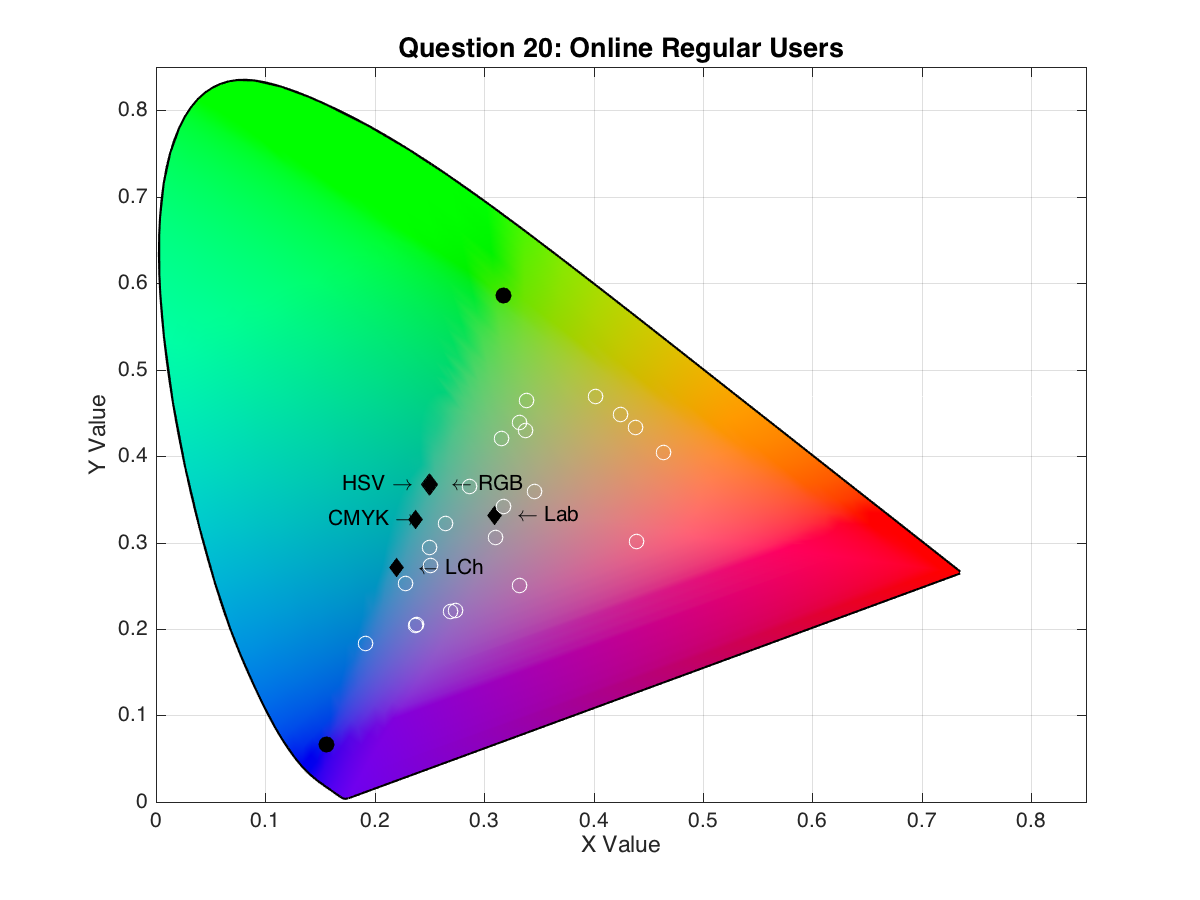
\includegraphics[width=0.7\textwidth]{images/20_online_regularUsers.png}
    \caption[Online Results: Answers for Question 20, from regular users.]{Online Results: Answers for Question 20, from regular users.}
    \label{fig:onlineregular_20}
  \end{figure}
  %
  \item \ul{Distances} - Comparing the mean distances obtained previously on Table \ref{table:colormodels_distances_labonline_statistics} which were obtained by questions one to seventeen, the distances generated
  by the answers from questions eighteen to thirty-two are a bit higher on the HSV Color Model. However, this could be due to the fact \textbf{we have only presented discretized colors as options, and did not
  leave any wiggle-room for the user to indicate other colors which he thought it could be more appropriate}; moreover, this could be related to \textbf{users tended to explore and choose answers from other color
  models, instead of HSV possible answers}. Even so, the values are similar to the previous studied, being only the HSV and CMYK mean values higher than previously ($\tilde{x}_{HSV} = 0.18$, $\tilde{x}_{CMYK} = 0.13$).\\
  Blending \ul{Cyan and Yellow to produce green} is an example of a question which had one a higher value ($\tilde{x}_{Green = Cyan + Yellow} = 0.11$) when asked the user to indicate the blending-basis with subsequential
  blending in CIE-L*a*b* (question seventeen), and when it was asked the result of the same blending (question nineteen), it provided one of the lowest mean distance values when compared to the ideal CIE-L*a*b* response
  ($\tilde{x}_{Cyan + Yellow = Green} = 0.05$); this example if pictured in Figures
  \ref{fig:onlinelabregular_17} and \ref{fig:onlineregular_32}.
  %
  \begin{figure}[!htbp]
    \centering
    \begin{minipage}{0.48\textwidth}
      \centering
      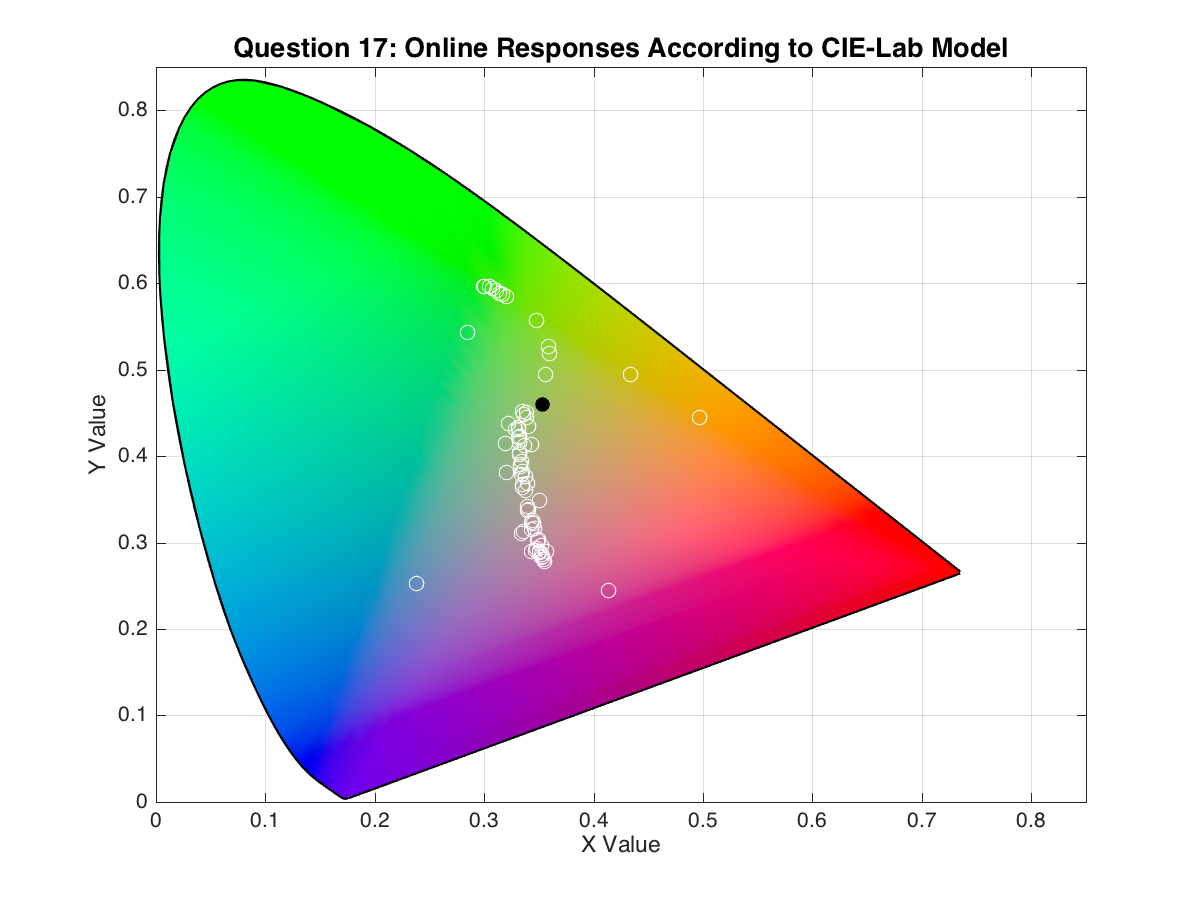
\includegraphics[width=\textwidth]{images/17_online_Labresponses.png}
      \caption[Online Results: Answers for Question 17, from regular users, mixed in CIE-L*a*b* Color Model.]{Online Results: Answers for Question 17, from regular users, mixed in CIE-L*a*b* Color Model.}
      \label{fig:onlinelabregular_17}
    \end{minipage}\hfill
    \begin{minipage}{0.48\textwidth}
      \centering
      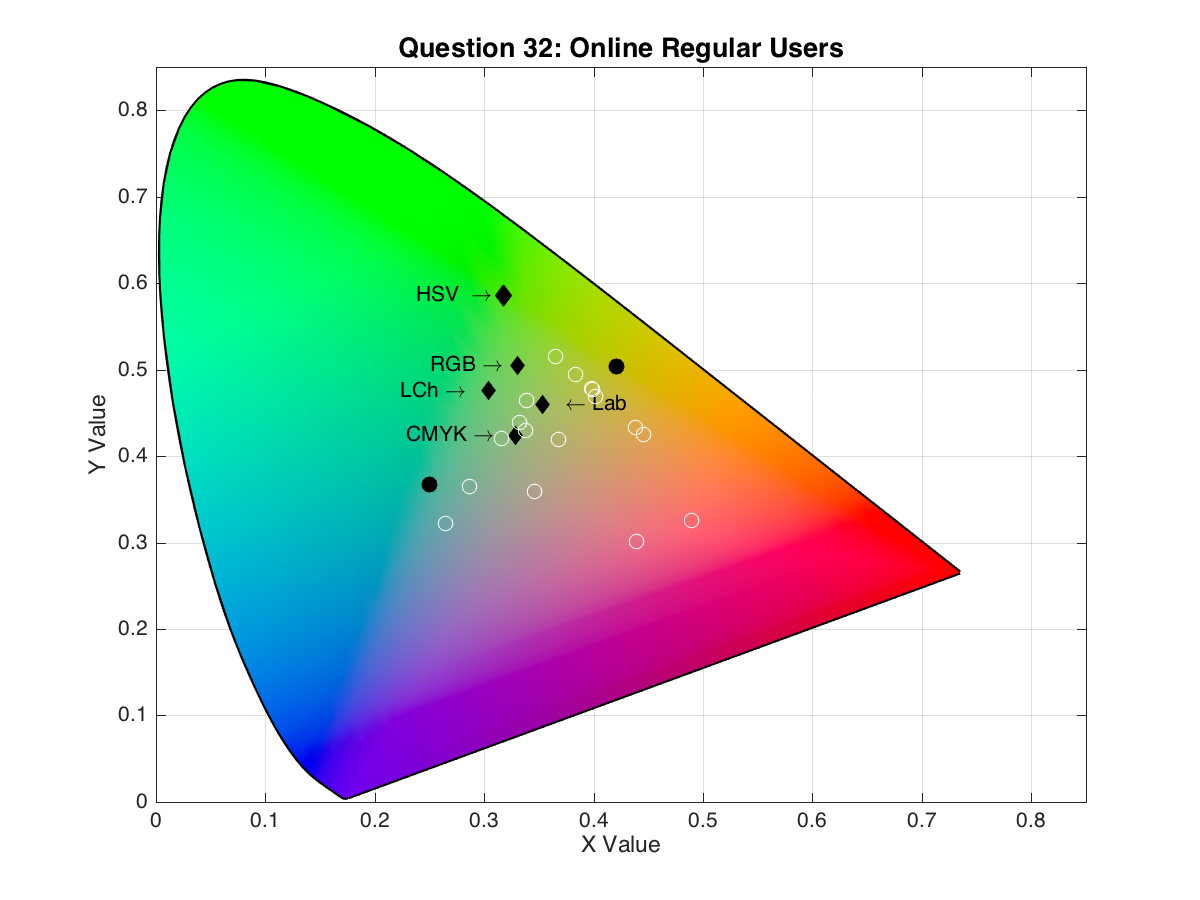
\includegraphics[width=\textwidth]{images/32_online_regularUsers.png}
      \caption[Online Results: Answers for Question 32, from regular users.]{Online Results: Answers for Question 32, from regular users.}
      \label{fig:onlineregular_32}
    \end{minipage}
  \end{figure}
  %
  \item \ul{Orange Blending} - Comparing the results from all questions, we end up concluding that the question which constantly had best results among all color models was the blending of red and yellow to create
  orange. However, as it is observable, these results represent much higher distances to the ideal answer in any color model, than when given the user the resulting color of the blending. This fact could indiciate
  that \textbf{it is harder for the users to detect the result of a color blend, when two blending basis are given, than when the resulting color is given}, even for the orange color blending which produced great
  results in the previous analysis. This could be related to the lack of descriptive power which the color slider supplied the user, which was referred before. This conclusion is corroborated by the online users which,
  although generating lower mean values than the laboratory ones, are coeherent with being higher than the ones previously studied.
  %
  \item \ul{Blue Blending} - Recalling the previous analysis, the results for mixtures which resulted in a blue shade all had the worst results among all questions, across all color models. \emph{Per contra}, the
  results for questions which present a blending basis for creating a blue color had presented much closer distances than before. For example, question twenty-four presented \ul{Cyan and Magenta} seeking a \ul{Blue}
  answer: when the users were asked to indicate the basis (question seven), it generated higher standard deviations which are illustrated in Table \ref{table:colormodels_distances_questions_statistics}. However, as
  seen on Table \ref{table:cyanmagenta_blue_analysis}, the results substantially improve when the users were asked to formulate the result of such blending. \\
  This could potentially suggest that \textbf{according to the users' expectation, it is easier for them to indicate the result of a blue mixture when the blending-basis is given, than when the user is asked
  to create the blending-basis according to their mental color model}.
  %
  \begin{table}[H]
    \resizebox{\textwidth}{!} {
    \begin{tabular}{ccccccccccccc}
      \hline
      \multicolumn{2}{c}{}                                        &                                                          & \multicolumn{10}{c}{Results}                                                                                                                                                                                                                                                                                                                                                                                                                                                                                                                                                             \\ \cline{4-13}
      \multicolumn{2}{c}{\multirow{-2}{*}{Blending Basis}}        & \multirow{-2}{*}{Resulting Color}                        & \multicolumn{2}{c}{HSV}                                                                                              & \multicolumn{2}{c}{CIE-L*C*h}                                                                                        & \multicolumn{2}{c}{CMYK}                                                                                             & \multicolumn{2}{c}{RGB}                                                                                              & \multicolumn{2}{c}{CIE-L*a*b*}                                                               \\ \hline
      Cyan & \multicolumn{1}{c|}{\cellcolor[HTML]{FFFFFF}Magenta} & \multicolumn{1}{c|}{\cellcolor[HTML]{0000FF}(18, 7, 95)} & \cellcolor[HTML]{FFFFFF}Laboratory ($\tilde{x}$) & \multicolumn{1}{c|}{\cellcolor[HTML]{FFFFFF}Online ($\tilde{x}$)} & \cellcolor[HTML]{FFFFFF}Laboratory ($\tilde{x}$) & \multicolumn{1}{c|}{\cellcolor[HTML]{FFFFFF}Online ($\tilde{x}$)} & \cellcolor[HTML]{FFFFFF}Laboratory ($\tilde{x}$) & \multicolumn{1}{c|}{\cellcolor[HTML]{FFFFFF}Online ($\tilde{x}$)} & \cellcolor[HTML]{FFFFFF}Laboratory ($\tilde{x}$) & \multicolumn{1}{c|}{\cellcolor[HTML]{FFFFFF}Online ($\tilde{x}$)} & \cellcolor[HTML]{FFFFFF}Laboratory ($\tilde{x}$) & \multicolumn{1}{c|}{Online ($\tilde{x}$)} \\ \hline
      \multicolumn{3}{l|}{Given Result, Expected Basis}                                                                      & \textbf{0.16}                                    & \multicolumn{1}{c|}{\textbf{0.13}}                                & 0.23                                             & \multicolumn{1}{c|}{0.18}                                         & 0.10                                             & \multicolumn{1}{c|}{0.11}                                         & 0.15                                             & \multicolumn{1}{c|}{0.17}                                         & 0.17                                             & \multicolumn{1}{c|}{0.22}                 \\
      \multicolumn{3}{l|}{Given Basis, Expected Result}                                                                      & 0.27                                             & \multicolumn{1}{c|}{0.28}                                         & \textbf{0.12}                                    & \multicolumn{1}{c|}{\textbf{0.11}}                                & \textbf{0.08}                                    & \multicolumn{1}{c|}{\textbf{0.09}}                                & \textbf{0.12}                                    & \multicolumn{1}{c|}{\textbf{0.13}}                                & \textbf{0.08}                                    & \multicolumn{1}{c|}{\textbf{0.09}}        \\ \hline
    \end{tabular}}
    \caption[Results of Blending Cyan and Magenta, obtaining Blue.]{Results of Blending Cyan and Magenta, obtaining Blue.}
    \label{table:cyanmagenta_blue_analysis}
  \end{table}
  %
  \item \ul{Color Models Analysis} - There were some changes concerning the descriptive statistics associated with distances values from each color model, specially when discovering which models yielded the best and
  worst results. To help us establish the comparisons between color models, we created an auxiliary Table (\ref{table:colormodels_expectations_labonline_statistics}) which contains the values. Contrary to questions in
  which the user was asked to indicate the blending basis, \textbf{the color model which has the worst results is the HSV Color Model} ($\tilde{x}_{HSV} = 0.18$) while the one which has \textbf{the shortest mean distance
  value continues to be CMYK, along with CIE-L*a*b*} ($\tilde{x} = 0.13$). Though, when processing the values for the whole statistics, RGB Color Model turns out to be the one which contains the best results: this not only
  is confirmed by the online users' data, but also is contrary to the results from the first analysis which dictated that the best color model was CMYK. This is particularly interesting, since it reveals that \textbf{when
  the users are asked to combine colors after a resulting one is given, they tend to blend according to a subtractive color model (\emph{e.g.} CMYK); but, when the blending-basis is given, the users are likely to mix the colors
  according to an addictive color model (\emph{e.g. RGB})}. \\
  On its turn, CIE-L*C*h* continues to reveal itself as the worst-valued Color Model, having the highest standard deviation ($\sigma = 0.07$), the highest range of distances ($range = 0.22$) and the highest variance of values
  ($\sigma^2 = 0.005$), across both study environments.
  %
  \begin{table}[htbp]
    \resizebox{\textwidth}{!} {
    \begin{tabular}{@{}ccccccccccc@{}}
      \toprule
                                                                                         & \multicolumn{5}{c}{Laboratory Environment}                                                                                                                                                                                   & \multicolumn{5}{c}{Online Environment}                                                                                                                                                                               \\ \cmidrule(l){2-11}
      \multirow{-2}{*}{\begin{tabular}[c]{@{}c@{}}Descriptive\\ Statistics\end{tabular}} & HSV                                   & CIE-L*C*h*                             & CMYK                                  & RGB                                    & CIE-L*a*b*                                                 & HSV                                   & CIE-L*C*h*                             & CMYK                                  & RGB                                    & CIE-L*a*b*                                         \\ \midrule
      \multicolumn{1}{c|}{Mean ($\tilde{x}$)}                                            & \cellcolor[HTML]{CB0000}\textbf{0.18} & \cellcolor[HTML]{FFFFFF}0.17           & \cellcolor[HTML]{32CB00}\textbf{0.13} & \cellcolor[HTML]{FFFFFF}0.14           & \multicolumn{1}{c|}{\cellcolor[HTML]{32CB00}\textbf{0.13}} & \cellcolor[HTML]{CB0000}\textbf{0.17} & \cellcolor[HTML]{FFFFFF}0.15           & \cellcolor[HTML]{32CB00}\textbf{0.11} & \cellcolor[HTML]{FFFFFF}0.13           & \multicolumn{1}{c|}{\cellcolor[HTML]{FFFFFF}0.12}  \\ \midrule
      \multicolumn{1}{l|}{Std-Dev ($\sigma$)}                                            & \cellcolor[HTML]{FFFFFF}0.06          & \cellcolor[HTML]{CB0000}\textbf{0.07}  & \cellcolor[HTML]{FFFFFF}0.04          & \cellcolor[HTML]{32CB00}\textbf{0.03}  & \multicolumn{1}{c|}{\cellcolor[HTML]{FFFFFF}0.04}          & \cellcolor[HTML]{CB0000}\textbf{0.07} & \cellcolor[HTML]{CB0000}\textbf{0.07}  & \cellcolor[HTML]{FFFFFF}0.04          & \cellcolor[HTML]{32CB00}\textbf{0.03}  & \multicolumn{1}{c|}{\cellcolor[HTML]{FFFFFF}0.04}  \\ \midrule
      \multicolumn{1}{c|}{Maximum Value}                                                 & \cellcolor[HTML]{FFFFFF}0.28          & \cellcolor[HTML]{FFFFFF}0.29           & \cellcolor[HTML]{FFFFFF}0.25          & \cellcolor[HTML]{FFFFFF}0.21           & \multicolumn{1}{c|}{\cellcolor[HTML]{FFFFFF}0.20}          & \cellcolor[HTML]{FFFFFF}0.29          & \cellcolor[HTML]{FFFFFF}0.29           & \cellcolor[HTML]{FFFFFF}0.20          & \cellcolor[HTML]{FFFFFF}0.17           & \multicolumn{1}{c|}{\cellcolor[HTML]{FFFFFF}0.19}  \\ \midrule
      \multicolumn{1}{c|}{Minimum Value}                                                 & \cellcolor[HTML]{FFFFFF}0.11          & \cellcolor[HTML]{FFFFFF}0.07           & \cellcolor[HTML]{FFFFFF}0.08          & \cellcolor[HTML]{FFFFFF}0.09           & \multicolumn{1}{c|}{\cellcolor[HTML]{FFFFFF}0.07}          & \cellcolor[HTML]{FFFFFF}0.09          & \cellcolor[HTML]{FFFFFF}0.07           & \cellcolor[HTML]{FFFFFF}0.07          & \cellcolor[HTML]{FFFFFF}0.07           & \multicolumn{1}{c|}{\cellcolor[HTML]{FFFFFF}0.05}  \\ \midrule
      \multicolumn{1}{c|}{Range}                                                         & \cellcolor[HTML]{FFFFFF}0.17          & \cellcolor[HTML]{CB0000}\textbf{0.22}  & \cellcolor[HTML]{FFFFFF}0.17          & \cellcolor[HTML]{32CB00}\textbf{0.12}  & \multicolumn{1}{c|}{\cellcolor[HTML]{FFFFFF}0.13}          & \cellcolor[HTML]{FFFFFF}0.20          & \cellcolor[HTML]{CB0000}\textbf{0.22}  & \cellcolor[HTML]{FFFFFF}0.13          & \cellcolor[HTML]{32CB00}\textbf{0.10}  & \multicolumn{1}{c|}{\cellcolor[HTML]{FFFFFF}0.14}  \\ \midrule
      \multicolumn{1}{c|}{Variance ($\sigma^2$)}                                                      & \cellcolor[HTML]{FFFFFF}0.003         & \cellcolor[HTML]{CB0000}\textbf{0.005} & \cellcolor[HTML]{FFFFFF}0.002         & \cellcolor[HTML]{32CB00}\textbf{0.001} & \multicolumn{1}{c|}{\cellcolor[HTML]{FFFFFF}0.002}         & \cellcolor[HTML]{FFFFFF}0.004         & \cellcolor[HTML]{CB0000}\textbf{0.005} & \cellcolor[HTML]{FFFFFF}0.002         & \cellcolor[HTML]{32CB00}\textbf{0.001} & \multicolumn{1}{c|}{\cellcolor[HTML]{FFFFFF}0.002} \\ \bottomrule
    \end{tabular}}
    \caption[Condensed Statistics for Distances to Ideal Results, according to each Color Model, for questions 18 to 32.]{Condensed Statistics for Distances to Ideal Results, according to each Color Model, for questions 18 to 32. In Green/Red shade, the best/worst result for each descriptive statistic.}
    \label{table:colormodels_expectations_labonline_statistics}
  \end{table}
  %
\end{itemize}
%
Therefore, we can summarize the results in one table, which ranks the color models \emph{per} color blending, dividing it between two strands: based on the values that represent questions in which the user was
asked to indicate the blending-basis, and based on the values that represent questions in which the user was asked to point out the correct blending result when given two colors. These results are presented in
table \ref{table:blendings_models_rank}. The color models were ranked according to the descriptive statistics' values generated by each question, weighted with the results from the laboratory environment and the
validation from the online users; marked in \textbf{bold} are the color models which we have concluded to yield the best results, according to each type of question asked.
%
\begin{table}[htbp]
  \resizebox{\textwidth}{!} {
  \begin{tabular}{@{}cccccccccccccc@{}}
    \toprule
    \multicolumn{2}{c}{Blending Basis}     & \multicolumn{2}{c}{Blending Result}                                                                                   & \multicolumn{5}{c}{Given the Result, Asked for Basis}                                                                                                                         & \multicolumn{5}{c}{Given the Basis, Asked for Result}                                                                                                                                  \\ \midrule
    C1      & C2                           & \multicolumn{2}{c|}{C3}                                                                                               & \#1                                & \#2                                & \#3                             & \#4                             & \multicolumn{1}{c|}{\#5}        & \#1                                & \#2                                & \#3                                & \#4                                & \multicolumn{1}{c|}{\#5}           \\ \midrule
    Red     & \multicolumn{1}{c|}{Green}   & \multicolumn{2}{c|}{\cellcolor[HTML]{FFFF00}(77, 93, 14)}                                                             & \multicolumn{1}{c|}{\textbf{CMYK}} & \multicolumn{1}{c|}{CIE-L*a*b*}    & \multicolumn{1}{c|}{RGB}        & \multicolumn{1}{c|}{HSV}        & \multicolumn{1}{c|}{CIE-L*C*h*} & \multicolumn{1}{c|}{\textbf{CMYK}} & \multicolumn{1}{c|}{CIE-L*a*b*}    & \multicolumn{1}{c|}{HSV}           & \multicolumn{1}{c|}{\textbf{RGB}}  & \multicolumn{1}{c|}{CIE-L*C*h*}    \\ \midrule
    Red     & \multicolumn{1}{c|}{Blue}    & \multicolumn{2}{c|}{\cellcolor[HTML]{FF00FF}(59, 28, 97)}                                                             & \multicolumn{1}{c|}{\textbf{CMYK}} & \multicolumn{1}{c|}{CIE-L*a*b*}    & \multicolumn{1}{c|}{CIE-L*C*h*} & \multicolumn{1}{c|}{RGB}        & \multicolumn{1}{c|}{HSV}        & \multicolumn{1}{c|}{HSV}           & \multicolumn{1}{c|}{\textbf{RGB}}  & \multicolumn{1}{c|}{\textbf{CMYK}} & \multicolumn{1}{c|}{CIE-L*a*b*}    & \multicolumn{1}{c|}{CIE-L*C*h*}    \\ \midrule
    Green   & \multicolumn{1}{c|}{Blue}    & \multicolumn{2}{c|}{\cellcolor[HTML]{00FFFF}(54, 79, 107)}                                                            & \multicolumn{5}{c|}{-}                                                                                                                                                        & \multicolumn{1}{c|}{CIE-L*a*b*}    & \multicolumn{2}{c|}{\textbf{HSV, RGB}}                                  & \multicolumn{1}{c|}{\textbf{CMYK}} & \multicolumn{1}{c|}{CIE-L*C*h*}    \\ \midrule
    Red     & \multicolumn{1}{c|}{Cyan}    & \multicolumn{1}{c|}{\cellcolor[HTML]{80FF00}(45, 76, 12)} & \multicolumn{1}{c|}{\cellcolor[HTML]{7F00FF}(27, 12, 95)} & \multicolumn{1}{c|}{\textbf{CMYK}} & \multicolumn{1}{c|}{HSV}           & \multicolumn{1}{c|}{RGB}        & \multicolumn{1}{c|}{CIE-L*a*b*} & \multicolumn{1}{c|}{CIE-L*C*h*} & \multicolumn{1}{c|}{\textbf{RGB}}  & \multicolumn{1}{c|}{\textbf{CMYK}} & \multicolumn{1}{c|}{CIE-L*a*b*}    & \multicolumn{1}{c|}{HSV}           & \multicolumn{1}{c|}{CIE-L*C*h*}    \\ \midrule
    Red     & \multicolumn{1}{c|}{Magenta} & \multicolumn{2}{c|}{\cellcolor[HTML]{FF0080}(45, 23, 22)}                                                             & \multicolumn{1}{c|}{\textbf{CMYK}} & \multicolumn{1}{c|}{CIE-L*a*b*}    & \multicolumn{1}{c|}{RGB}        & \multicolumn{1}{c|}{CIE-L*C*h*} & \multicolumn{1}{c|}{HSV}        & \multicolumn{1}{c|}{HSV}           & \multicolumn{2}{c|}{CIE-L*C*h*, CIE-L*a*b*}                             & \multicolumn{1}{c|}{\textbf{RGB}}  & \multicolumn{1}{c|}{\textbf{CMYK}} \\ \midrule
    Red     & \multicolumn{1}{c|}{Yellow}  & \multicolumn{2}{c|}{\cellcolor[HTML]{FF8000}(49, 37, 5)}                                                              & \multicolumn{1}{c|}{CIE-L*a*b*}    & \multicolumn{1}{c|}{\textbf{CMYK}} & \multicolumn{1}{c|}{HSV}        & \multicolumn{1}{c|}{RGB}        & \multicolumn{1}{c|}{CIE-L*C*h*} & \multicolumn{3}{c|}{\textbf{CMYK, CIE-L*C*h*, CIE-L*a*b*}}                                                   & \multicolumn{1}{c|}{HSV}           & \multicolumn{1}{c|}{\textbf{RGB}}  \\ \midrule
    Cyan    & \multicolumn{1}{c|}{Magenta} & \multicolumn{2}{c|}{\cellcolor[HTML]{0000FF}(18, 7, 95)}                                                              & \multicolumn{5}{c|}{Inconclusive Results}                                                                                                                                     & \multicolumn{2}{c|}{\textbf{CMYK, CIE-L*a*b*}}                          & \multicolumn{1}{c|}{CIE-L*C*h*}    & \multicolumn{1}{c|}{\textbf{RGB}}  & \multicolumn{1}{c|}{HSV}           \\ \midrule
    Magenta & \multicolumn{1}{c|}{Yellow}  & \multicolumn{2}{c|}{\cellcolor[HTML]{FF0000}(41, 21, 2)}                                                              & \multicolumn{1}{c|}{\textbf{CMYK}} & \multicolumn{1}{c|}{CIE-L*C*h*}    & \multicolumn{1}{c|}{HSV}        & \multicolumn{1}{c|}{RGB}        & \multicolumn{1}{c|}{CIE-L*a*b*} & \multicolumn{1}{c|}{CIE-L*a*b*}    & \multicolumn{1}{c|}{\textbf{CMYK}} & \multicolumn{1}{c|}{\textbf{RGB}}  & \multicolumn{1}{c|}{CIE-L*C*h*}    & \multicolumn{1}{c|}{HSV}           \\ \midrule
    Green   & \multicolumn{1}{c|}{Cyan}    & \multicolumn{2}{c|}{\cellcolor[HTML]{00FF80}(40, 73, 32)}                                                             & \multicolumn{1}{c|}{\textbf{CMYK}} & \multicolumn{1}{c|}{RGB}           & \multicolumn{1}{c|}{CIE-L*a*b*} & \multicolumn{1}{c|}{HSV}        & \multicolumn{1}{c|}{CIE-L*C*h*} & \multicolumn{1}{c|}{CIE-L*C*h*}    & \multicolumn{1}{c|}{\textbf{CMYK}} & \multicolumn{1}{c|}{CIE-L*a*b*}    & \multicolumn{1}{c|}{HSV}           & \multicolumn{1}{c|}{\textbf{RGB}}  \\ \midrule
    Green   & \multicolumn{1}{c|}{Magenta} & \multicolumn{1}{c|}{\cellcolor[HTML]{0080FF}(26, 23, 98)} & \multicolumn{1}{c|}{\cellcolor[HTML]{FF8000}(49, 37, 5)}  & \multicolumn{1}{c|}{\textbf{CMYK}} & \multicolumn{1}{c|}{RGB}           & \multicolumn{1}{c|}{CIE-L*a*b*} & \multicolumn{1}{c|}{HSV}        & \multicolumn{1}{c|}{CIE-L*C*h*} & \multicolumn{1}{c|}{\textbf{RGB}}  & \multicolumn{1}{c|}{\textbf{CMYK}} & \multicolumn{1}{c|}{CIE-L*a*b*}    & \multicolumn{1}{c|}{HSV}           & \multicolumn{1}{c|}{CIE-L*C*h*}    \\ \midrule
    Green   & \multicolumn{1}{c|}{Yellow}  & \multicolumn{2}{c|}{\cellcolor[HTML]{80FF00}(45, 76, 12)}                                                             & \multicolumn{1}{c|}{HSV}           & \multicolumn{1}{c|}{\textbf{CMYK}} & \multicolumn{1}{c|}{RGB}        & \multicolumn{1}{c|}{CIE-L*a*b*} & \multicolumn{1}{c|}{CIE-L*C*h*} & \multicolumn{1}{c|}{\textbf{CMYK}} & \multicolumn{2}{c|}{CIE-L*C*h*, CIE-L*a*b*}                             & \multicolumn{1}{c|}{\textbf{RGB}}  & \multicolumn{1}{c|}{HSV}           \\ \midrule
    Blue    & \multicolumn{1}{c|}{Cyan}    & \multicolumn{2}{c|}{\cellcolor[HTML]{0080FF}(26, 23, 98)}                                                             & \multicolumn{5}{c|}{Inconclusive Results}                                                                                                                                     & \multicolumn{1}{c|}{CIE-L*C*h*}    & \multicolumn{1}{c|}{CIE-L*a*b*}    & \multicolumn{1}{c|}{\textbf{CMYK}} & \multicolumn{2}{c|}{\textbf{HSV, RGB}}                                  \\ \midrule
    Blue    & \multicolumn{1}{c|}{Magenta} & \multicolumn{2}{c|}{\cellcolor[HTML]{8000FF}(27, 12, 95)}                                                             & \multicolumn{1}{c|}{\textbf{CMYK}} & \multicolumn{1}{c|}{HSV}           & \multicolumn{1}{c|}{RGB}        & \multicolumn{1}{c|}{CIE-L*a*b*} & \multicolumn{1}{c|}{CIE-L*C*h*} & \multicolumn{2}{c|}{CIE-L*C*h*, CIE-L*a*b*}                             & \multicolumn{1}{c|}{\textbf{CMYK}} & \multicolumn{1}{c|}{\textbf{RGB}}  & \multicolumn{1}{c|}{HSV}           \\ \midrule
    Blue    & \multicolumn{1}{c|}{Yellow}  & \multicolumn{1}{c|}{\cellcolor[HTML]{00FF80}(40, 73, 32)} & \multicolumn{1}{l|}{\cellcolor[HTML]{FF007F}(45, 23, 22)} & \multicolumn{1}{c|}{\textbf{CMYK}} & \multicolumn{1}{c|}{RGB}           & \multicolumn{1}{c|}{HSV}        & \multicolumn{1}{c|}{CIE-L*a*b*} & \multicolumn{1}{c|}{CIE-L*C*h*} & \multicolumn{1}{c|}{\textbf{CMYK}} & \multicolumn{1}{c|}{\textbf{RGB}}  & \multicolumn{1}{c|}{HSV}           & \multicolumn{1}{c|}{CIE-L*a*b*}    & \multicolumn{1}{c|}{CIE-L*C*h*}    \\ \midrule
    Cyan    & \multicolumn{1}{c|}{Yellow}  & \multicolumn{2}{c|}{\cellcolor[HTML]{00FF00}(36, 72, 13)}                                                             & \multicolumn{1}{c|}{\textbf{CMYK}} & \multicolumn{1}{c|}{HSV}           & \multicolumn{1}{c|}{RGB}        & \multicolumn{1}{c|}{CIE-L*a*b*} & \multicolumn{1}{c|}{CIE-L*C*h*} & \multicolumn{1}{c|}{CIE-L*a*b*}    & \multicolumn{1}{c|}{\textbf{CMYK}} & \multicolumn{1}{c|}{CIE-L*C*h*}    & \multicolumn{1}{c|}{\textbf{RGB}}  & \multicolumn{1}{c|}{HSV}           \\ \bottomrule
  \end{tabular}}
  \caption[Colors Models, ranked from best to worst, associated to every color blending studied.]{Colors Models, ranked from best to worst, associated to every color blending studied.}
  \label{table:blendings_models_rank}
\end{table}
%
\subsection{Color Mixtures and Color Naming}
\label{subsec:results_colormixtures}
%
Being the color models covered in the extensive previous analysis, we are left to analyze and break down each color mixture, understanding if there is a particular color blending which has an added level of
difficulty. As stated on Section \ref{sec:impl_objectives}, it is also interesting to study if the users have a particular choice to order the colors when demonstrating their answers, given its implications on how to draft \ul{Information Visualization Artifacts},
such as sliders, scales or color blends to convey information.
%
This subsection will be composed on two main groups: on the first one, we will focus our attention on the color blendings which are \textbf{based on primary colors, to generate other primary colors} to comprehend
if the users can detect and formulate primary color blendings; the second group of this subsection will contain a \textbf{brief investigation about the difficulty found when blending colors}, focusing our attention
not only on each question, but also on providing a general perception of how the study went, regarding the facility of unveiling color mixtures. \par
%
We also performed a color analysis by comparing the colors given by our users, with the ones obtained with the XKCD's Color Bins referred on the \emph{Data Processing} section (\ref{subsec:results_preparation}) of this document. This way,
we can make sense out of the values, giving them meaning and necessary categorization. This is going to be useful when analyzing the proximity of values.
%
\subsubsection{Primary Colors}
\label{subsubsec:primarycolors}
%
Among all the questions proponed to the user, there were of six of them which presented as the result of a color mixture, either one of the following primary colors: \textbf{Red, Green, Blue, Cyan, Magenta,}
or \textbf{Yellow}. These results were created, as in other questions, by blending the primitives of the most common color models (RGB and CMYK) which, ultimately, happen to provide the primary colors which
formulate the ones referred in the beggining of this paragraph. These questions (\textbf{primary colors, formulated based on other primary colors}) are refreshed again on Table \ref{table:primary_blends}. \par
%
\begin{table}[htbp]
  \resizebox{\textwidth}{!} {
  \begin{tabular}{ccccclclclclcl}
    \hline
                                  & \multicolumn{2}{c}{Blending Basis}                          &                                                                          & \multicolumn{10}{c}{Possible Results}                                                                                                                                                                                                                                                                                                                                                                 \\ \cline{2-3} \cline{5-14}
    \multirow{-2}{*}{Question ID} & C1                           & C2                           & \multirow{-2}{*}{Blending Result}                                        & \multicolumn{2}{c}{HSV}                                                         & \multicolumn{2}{c}{CIE-L*C*h}                                                    & \multicolumn{2}{c}{CMYK}                                                         & \multicolumn{2}{c}{RGB}                                                          & \multicolumn{2}{c}{CIE-L*a*b*}                             \\ \hline
    \multicolumn{1}{c|}{8, 25}    & \multicolumn{1}{c|}{Magenta} & \multicolumn{1}{c||}{Yellow}  & \multicolumn{1}{c||}{\cellcolor[HTML]{FF0000}{\color[HTML]{FFFFFF} Red}}  & \multicolumn{2}{c||}{\cellcolor[HTML]{FF0000}{\color[HTML]{FFFFFF} (41, 21, 2)}} & \multicolumn{2}{c||}{\cellcolor[HTML]{FF6755}{\color[HTML]{FFFFFF} (48, 32, 12)}} & \multicolumn{2}{c||}{\cellcolor[HTML]{FF8080}{\color[HTML]{FFFFFF} (53, 38, 25)}} & \multicolumn{2}{c||}{\cellcolor[HTML]{FF8080}{\color[HTML]{FFFFFF} (53, 38, 25)}} & \multicolumn{2}{c|}{\cellcolor[HTML]{FFA6A6}(62, 51, 43)}  \\ \hline \hline
    \multicolumn{1}{c|}{17, 32}   & \multicolumn{1}{c|}{Cyan}    & \multicolumn{1}{c||}{Yellow}  & \multicolumn{1}{c||}{\cellcolor[HTML]{00FF00}Green}                       & \multicolumn{2}{c||}{\cellcolor[HTML]{00FF00}(36, 72, 13)}                       & \multicolumn{2}{c||}{\cellcolor[HTML]{6EFFA3}(49, 77, 47)}                        & \multicolumn{2}{c||}{\cellcolor[HTML]{80FF80}(49, 78, 33)}                        & \multicolumn{2}{c||}{\cellcolor[HTML]{80FF80}(49, 78, 33)}                        & \multicolumn{2}{c|}{\cellcolor[HTML]{C4FF9E}(66, 87, 46)}  \\ \hline \hline
    \multicolumn{1}{c|}{7, 24}    & \multicolumn{1}{c|}{Cyan}    & \multicolumn{1}{c||}{Magenta} & \multicolumn{1}{c||}{\cellcolor[HTML]{0000FF}{\color[HTML]{FFFFFF} Blue}} & \multicolumn{2}{c||}{\cellcolor[HTML]{0000FF}{\color[HTML]{FFFFFF} (18, 7, 95)}} & \multicolumn{2}{c||}{\cellcolor[HTML]{00CAFF}(39, 49, 102)}                       & \multicolumn{2}{c||}{\cellcolor[HTML]{8080FF}{\color[HTML]{FFFFFF} (35, 27, 98)}} & \multicolumn{2}{c||}{\cellcolor[HTML]{8080FF}{\color[HTML]{FFFFFF} (35, 27, 98)}} & \multicolumn{2}{c|}{\cellcolor[HTML]{C6AEFF}(56, 50, 101)} \\ \hline \hline
    \multicolumn{1}{c|}{20}       & \multicolumn{1}{c|}{Green}   & \multicolumn{1}{c||}{Blue}    & \multicolumn{1}{c||}{\cellcolor[HTML]{00FFFF}Cyan}                        & \multicolumn{2}{c||}{\cellcolor[HTML]{00FFFF}(54, 79, 107)}                      & \multicolumn{2}{c||}{\cellcolor[HTML]{00A5FF}(32, 34, 100)}                       & \multicolumn{2}{c||}{\cellcolor[HTML]{008080}(12, 17, 23)}                        & \multicolumn{2}{c||}{\cellcolor[HTML]{008080}(12, 17, 23)}                        & \multicolumn{2}{c|}{\cellcolor[HTML]{7D93A6}(26, 28, 40)}  \\ \hline \hline
    \multicolumn{1}{c|}{2, 19}    & \multicolumn{1}{c|}{Red}     & \multicolumn{1}{c||}{Blue}    & \multicolumn{1}{c||}{\cellcolor[HTML]{FF00FF}Magenta}                     & \multicolumn{2}{c||}{\cellcolor[HTML]{FF00FF}(59, 28, 97)}                       & \multicolumn{2}{c||}{\cellcolor[HTML]{FB0080}{\color[HTML]{FFFFFF} (44, 22, 22)}} & \multicolumn{2}{c||}{\cellcolor[HTML]{800080}{\color[HTML]{FFFFFF} (13, 6, 21)}}  & \multicolumn{2}{c||}{\cellcolor[HTML]{800080}{\color[HTML]{FFFFFF} (13, 6, 21)}}  & \multicolumn{2}{c|}{\cellcolor[HTML]{CA0088}(29, 14, 25)}  \\ \hline \hline
    \multicolumn{1}{c|}{1, 18}    & \multicolumn{1}{c|}{Red}     & \multicolumn{1}{c||}{Green}   & \multicolumn{1}{c||}{\cellcolor[HTML]{FFFF00}Yellow}                      & \multicolumn{2}{c||}{\cellcolor[HTML]{FFFF00}(77, 93, 14)}                       & \multicolumn{2}{c||}{\cellcolor[HTML]{D7A700}(42, 42, 6)}                         & \multicolumn{2}{c||}{\cellcolor[HTML]{808000}(17, 20, 3)}                         & \multicolumn{2}{c||}{\cellcolor[HTML]{808000}(17, 20, 3)}                         & \multicolumn{2}{c|}{\cellcolor[HTML]{C9AB00}(39, 42, 6)}   \\ \hline
  \end{tabular}}
  \caption[Color Blends based on Primary Colors, which result in other Primary Colors.]{Color Blends based on Primary Colors, which result in other Primary Colors.}
  \label{table:primary_blends}
\end{table}
%
As analyzed before, according to the users' responses and expectations, these questions show a fair degree of concordance when blending que mixture-basis, since they all tend tend to present better results when
blended according to a CMYK Color Model. However, we have found an interesting behaviour from our users when answering these questions: some users indicated the resulting color on both the expected colors (\emph{e.g.}
it was presented Red, and the users indicated twice the color Red in their answers); we will briefly analyze the values for each of the blendings referred on Table \ref{table:primary_blends}, as it has already been
analyzed before.
%
\paragraph{\ul{Magenta + Yellow = Red}}
%
In this question, it was expected that users indicate a mixing of Magenta and Yellow to blend in a result of Red. These colors are primitives from the CMYK Color Model which, when blended, generate a color from the
complementary color model, the RGB. However, the laboratory users did focus their answers on \textbf{orange, green, blue and even red hue}; moreover, these results were similar among the online users and did not
demonstrated a consensual answer pair. \\
%
Additionaly, five laboratory users (from thirteen which indicated a pair of two answers - $38.46\%$ of the users) and fourty-two online users (from sixty-two - $67.74\%$ of the users) indicated, at least, one time the
red color as an answer. We can even run some descriptive statistics on top of the \ul{distance values between the given answers and the expected Magenta-Yellow Pair} ($\tilde{x} = 0.49$, $\sigma = 0.25$) and observe that
these evidences lead us to believe that \textbf{the users do not know how to create a red color based on other primary colors}. \\
%
When analyzing question number twenty-five, in which we ask the user which color is the result of blending Magenta and Yellow, we conclude that \textbf{the results are, also,
scattered a bit}, which leads us to reinforce the statement above. \textbf{There is also no observable tendency to begin the color blending with a particular shade of a color}. Figures \ref{fig:redblend_1} and
\ref{fig:redblend_2} show us the answers given by the online users in, respectively, question eight and twenty-five.
%
\begin{figure}[!htbp]
  \centering
  \begin{minipage}{0.48\textwidth}
    \centering
    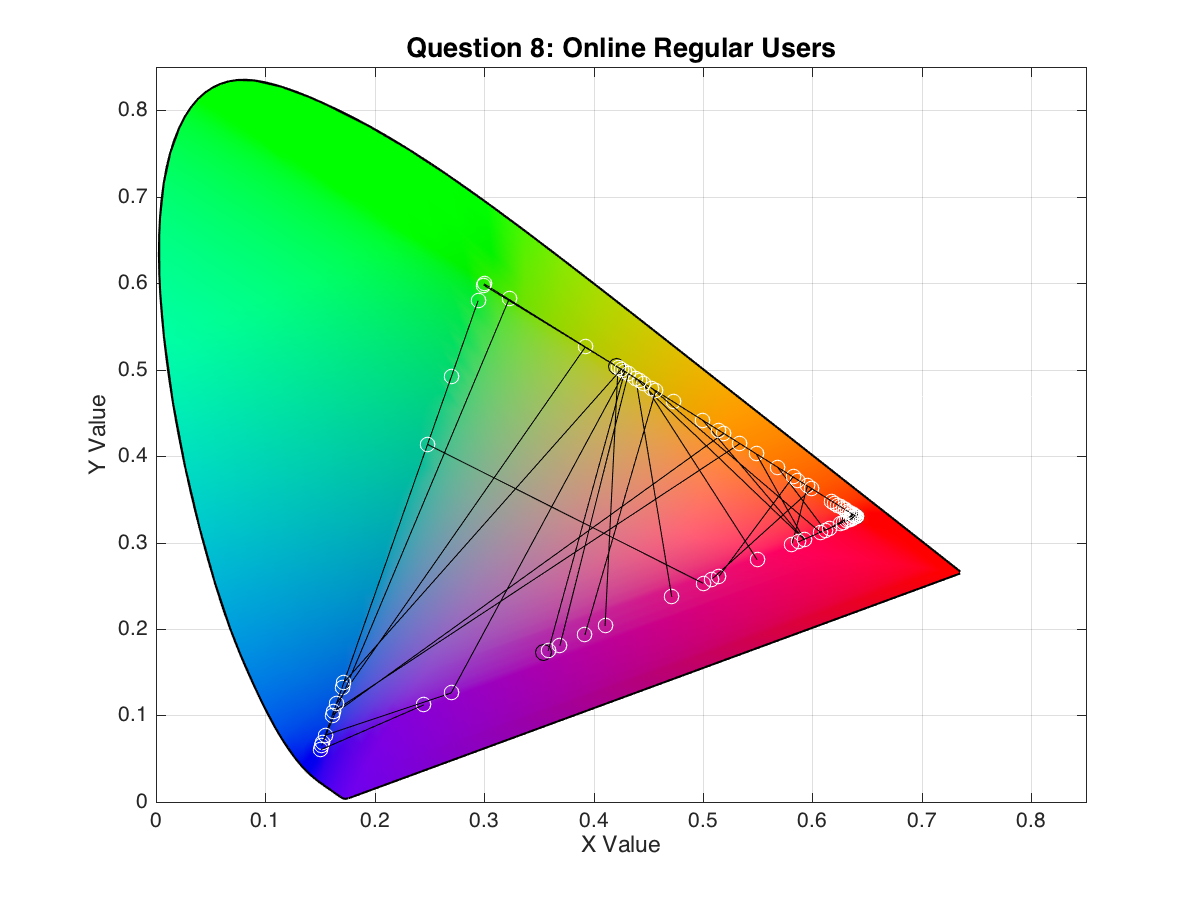
\includegraphics[width=\textwidth]{images/8_online_regularUsers.png}
    \caption[Online Results: Answers for Question 8, from regular users.]{Online Results: Answers for Question 8, from regular users.}
    \label{fig:redblend_1}
  \end{minipage}\hfill
  \begin{minipage}{0.48\textwidth}
    \centering
    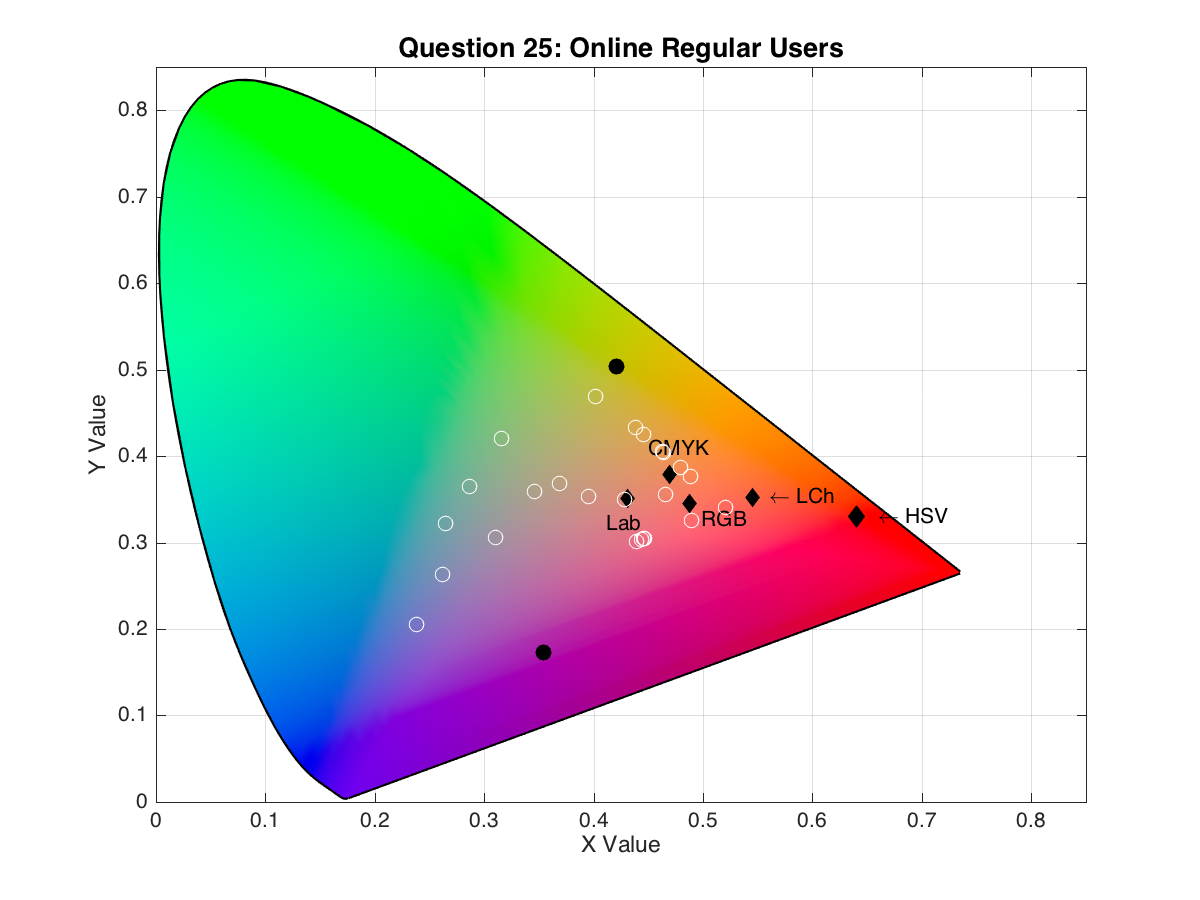
\includegraphics[width=\textwidth]{images/25_online_regularUsers.png}
    \caption[Online Results: Answers for Question 25, from regular users.]{Online Results: Answers for Question 25, from regular users.}
    \label{fig:redblend_2}
  \end{minipage}
\end{figure}
%
\paragraph{\ul{Cyan + Yellow = Green}}
%
Regarding this, it was expected that users indicate a mixing of Cyan and Yellow to blend in a result of Green. Similarly to the previous blend, these colors are primitives from the CMYK Color Model that, when blended,
generate a color from the RGB Color Model. Curiously, both the laboratory and online users provided their answers on similar pairs, comprised between \textbf{blue shades and yellow ones}; the most repeated
color pairs were, in fact, Blue shades combined with tones of green and yellow, as observable on Figure \ref{fig:greenblend_1}. \\
%
Additionaly, only two laboratory users (from twenty-three which indicated a pair of two answers - $8.70\%$ of the users) and six online users (from seventy-one - $8.45\%$ of the users) indicated an answer pair which did not even
nearly approximate to the desired hues. Running some descriptive statistics on top of the distance values between the given answers and the expected Magenta-Yellow Pair ($\tilde{x} = 0.40$, $\sigma = 0.21$) did reveal longer distances
also; however, since the majority of answers are near a cyan hue tending to a blue one, we consider these answers as valid ones. These evidences lead us to believe that \textbf{the users do present knowledge on how to create a green color
based on other primary colors, such as cyan/blue and yellow}. \\
%
When analyzing question number thirty-two, in which we ask the user which color is the result of blending Cyan and Yellow, we conclude that \textbf{the results, as previously happened with other primary blends, are a bit scattered}.
As before, \textbf{there is no observable tendency to begin the color blending with a particular shade of a color}. Figures \ref{fig:greenblend_2} and\ref{fig:greenblend_2} show us the answers given by the online users in, respectively,
question seventeen and thirty-two.
%
\begin{figure}[!htbp]
  \centering
  \begin{minipage}{0.48\textwidth}
    \centering
    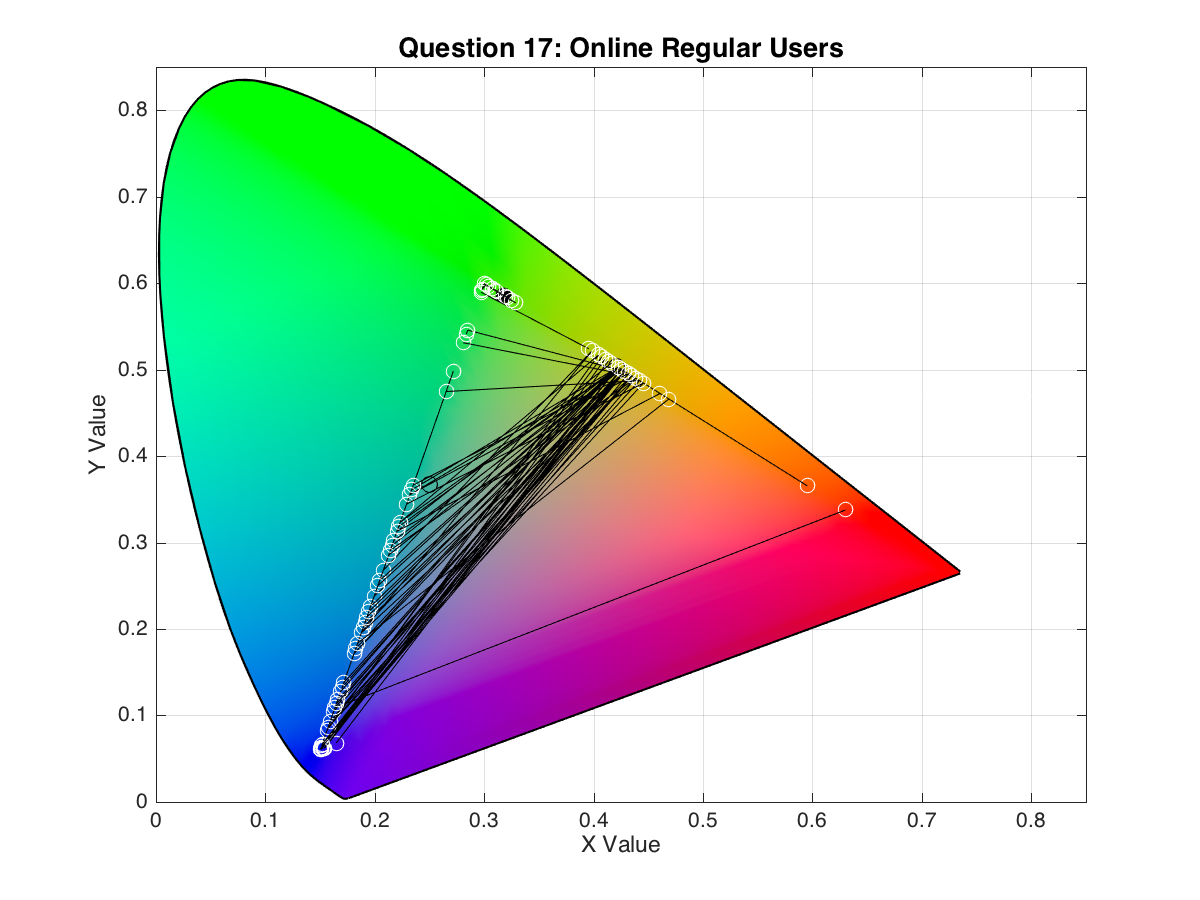
\includegraphics[width=\textwidth]{images/17_online_regularUsers.png}
    \caption[Online Results: Answers for Question 17, from regular users.]{Online Results: Answers for Question 17, from regular users.}
    \label{fig:greenblend_1}
  \end{minipage}\hfill
  \begin{minipage}{0.48\textwidth}
    \centering
    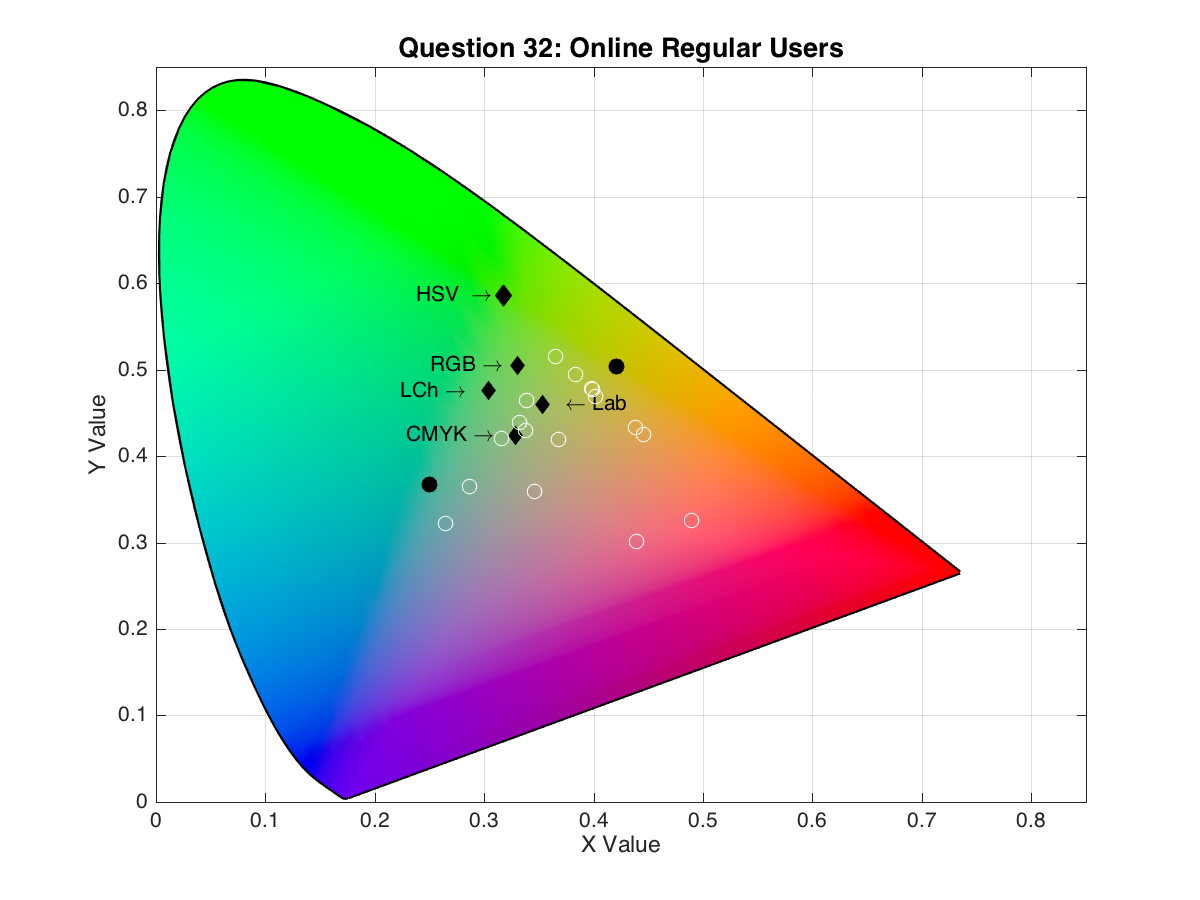
\includegraphics[width=\textwidth]{images/32_online_regularUsers.png}
    \caption[Online Results: Answers for Question 32, from regular users.]{Online Results: Answers for Question 32, from regular users.}
    \label{fig:greenblend_2}
  \end{minipage}
\end{figure}
%
\paragraph{\ul{Cyan + Magenta = Blue}}
%
In this question, it was expected that users indicate a mixing of Cyan and Magenta to blend in a result of Blue; these colors are primitives from the CMYK Color Model. Both the laboratory and online users provided their answers
on similar pairs, comprised between \textbf{blue shades, yellow ones, magenta's and pink, and some greens and reds}. There was also an interesting agregation of results on both environment, near the green and yellow shades.  \\
%
However, as seen on Figures \ref{fig:blueblend_1} and \ref{fig:blueblend_2} there exists a tendency of users indicating answers very close to the given color (Blue Hue). This could reveal an \textbf{inability of detecting a blue blending
basis}, which could be related to the (lack of) descriptive power among blue colors, previously referred. \\
5
Running some descriptive statistics on top of the distance values between the given answers and the expected Cyan-Magenta Pair ($\tilde{x} = 0.45$, $\sigma = 0.11$) reveals the same high mean distance value, but a lower than previous
standard deviation of results. Due to the fact that the users indicated some answers in the magenta zone of colors and some blue/cyan hues, we could state that \textbf{although there is no strong evidence to verify this color blending, the
users show a mild ability to blend cyan and magenta, providing a blue color}. \\
%
When analyzing question number twenty-four, in which we ask the user which color is the result of blending Cyan and Magenta, we conclude that \textbf{the results, as previously happened with other primary blends, are a bit scattered}.
As before, \textbf{there is no observable tendency to begin the color blending with a particular shade of a color}.
%
\begin{figure}[!htbp]
  \centering
  \begin{minipage}{0.48\textwidth}
    \centering
    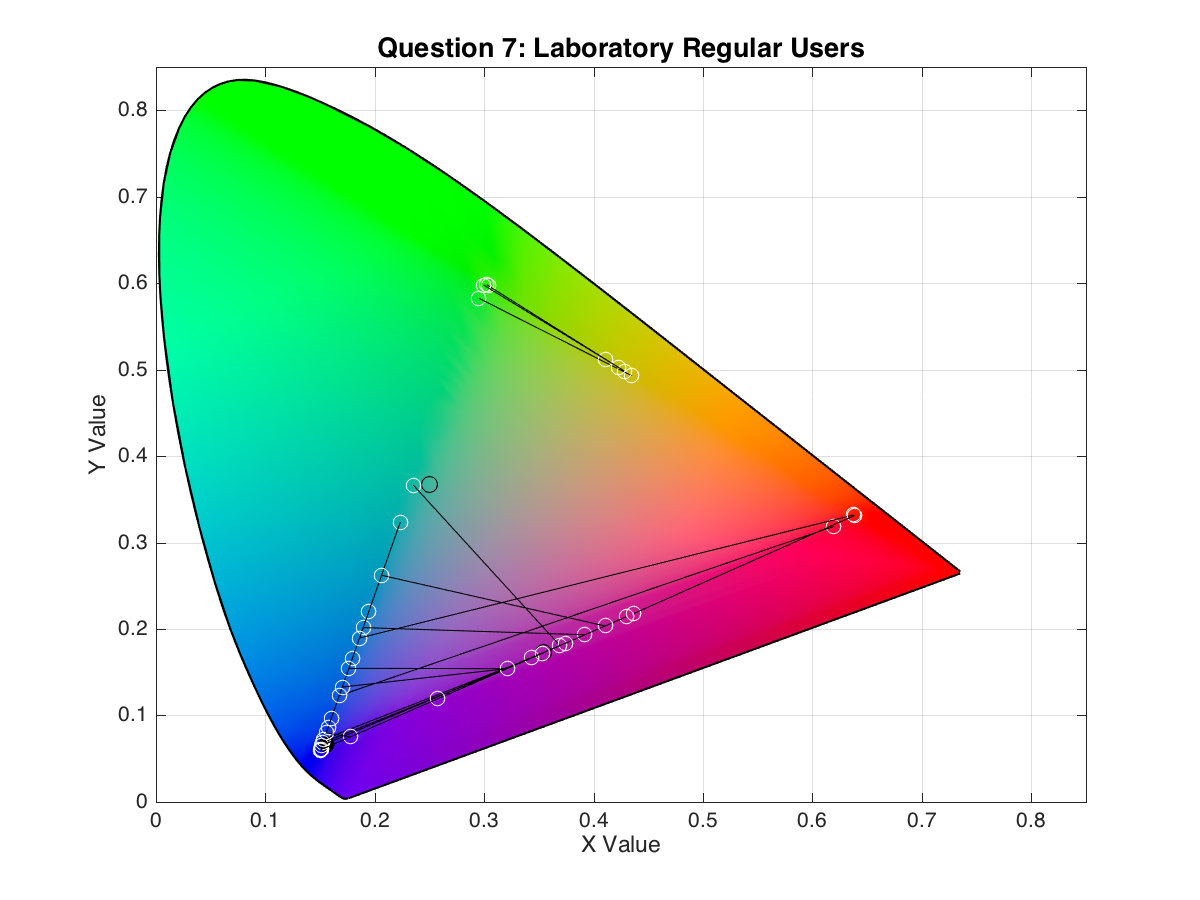
\includegraphics[width=\textwidth]{images/7_lab_regularUsers.png}
    \caption[Laboratory Results: Answers for Question 7, from regular users.]{Laboratory Results: Answers for Question 7, from regular users.}
    \label{fig:blueblend_1}
  \end{minipage}\hfill
  \begin{minipage}{0.48\textwidth}
    \centering
    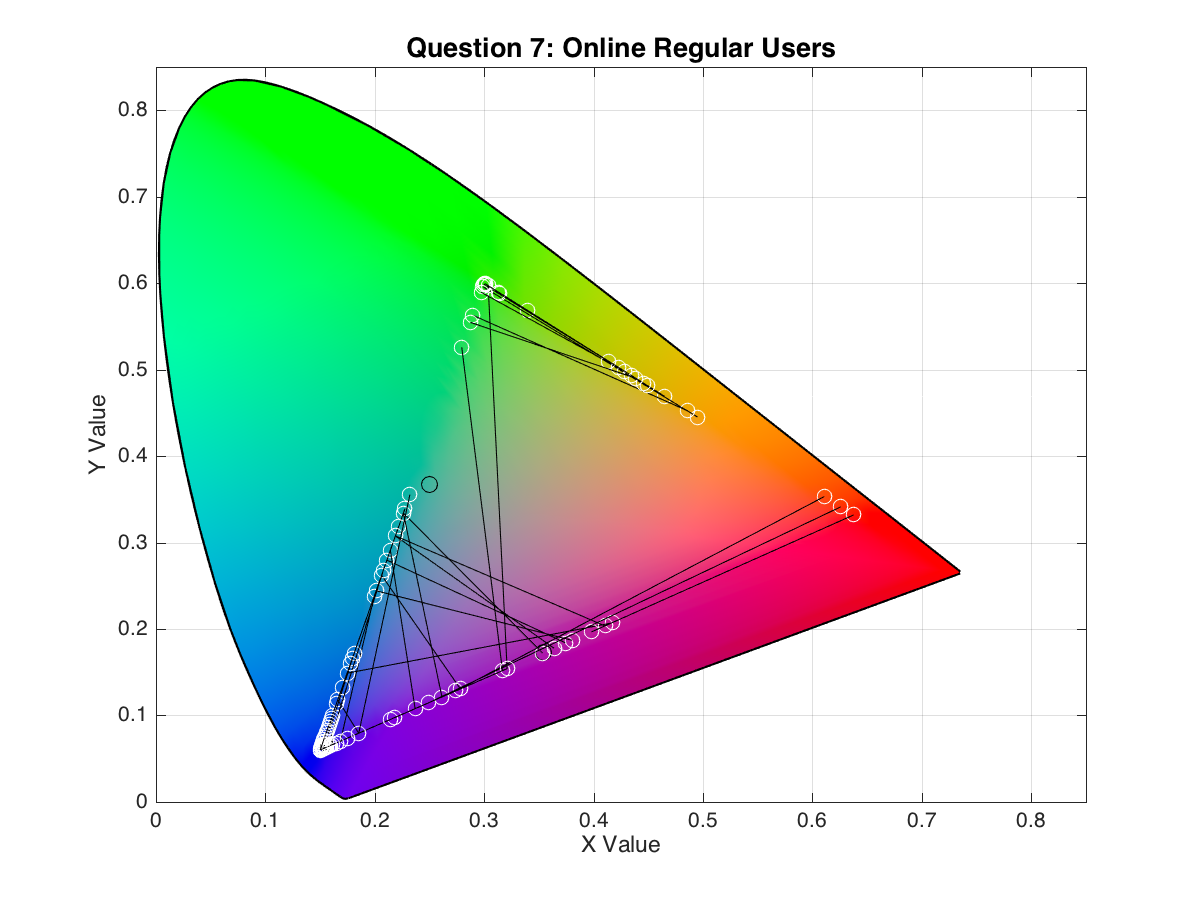
\includegraphics[width=\textwidth]{images/7_online_regularUsers.png}
    \caption[Online Results: Answers for Question 7, from regular users.]{Online Results: Answers for Question 7, from regular users.}
    \label{fig:blueblend_2}
  \end{minipage}
\end{figure}
%
\paragraph{\ul{Green + Blue = Cyan}}
%
As said before, this color blending was only conducted only in one way. In this question, it was expected that users indicate the result of mixing Green and Blue: Cyan; these colors are primitives from the RGB Color Model. Both the laboratory
and online users provided similar results, with an agregation of them on the blue and cyan hues on both environment, and also in the orange hue (for unknown reasons).  \\
%
Running some descriptive statistics on top of the distance values between the given answer and the expected Cyan Color ($\tilde{x} = 0.13$, $\sigma = 0.06$) reveals some proximity to the expected color, and a lower standard deviation of results.
Ideally, the results should be compared with the other type of question asked; since there is no question to compare and based on previous analyzed results, we can affirm that \textbf{there are mild evidences that users can detect a Green-Blue blend
to provide a Cyan color}. However, \textbf{further studies should deepen this question and determine if this affirmation could be corroborated}.
%
\paragraph{\ul{Red + Blue = Magenta}}
%
In this question, it was expected that users indicate a mixing of Red and Blue to mix in a result of Magenta. Both the laboratory and online users provided their answers on similar pairs, comprised between \textbf{blue shades, yellow ones, magenta's and
pink, and some greens and reds}. There was also an interesting agregation of results on both environment, \textbf{along the line which unites Blue and Red}, with some scattering among the cyan and teal colors.  \\
However, as seen on Figure \ref{fig:magentablend_1} there exists a tendency of users indicating answers very close to the given color (Blue Hue). This scattering of results could be related to the \textbf{blue blending
detection problems}, previously referred. \\
%
Running some descriptive statistics on top of the distance values between the given answers and the expected Red-Blue Pair ($\tilde{x} = 0.53$, $\sigma = 0.36$) reveals the highest mean distance value so far, and also a deviation of results higher than before.
the users indicated some scattered answers in the blue zone of the chromaticity diagram: answers include Light-Blue, Sky-Blue, Navy-Blue and Cyan, besides the typical Blue; on the other hand, the users have indicated spared answers in the Magenta zone: Dark-Purple,
Pink, Magenta and Red. This shattering of data is coherent with the deviation of values obtained: we could state that \textbf{the users demonstrated some basic conception of blending red and blue to obtain magenta}. However, \textbf{the users have indicated more
detailed colors, contrary to other color blends previously evaluated}, which may have implications on the level of detail that the displaying of color should have. \\
%
Analyzing question number nineteen, in which we ask the user which color is the result of blending Red and Blue, we conclude that \textbf{the results, as previously happened with other primary blends, are a bit scattered}, leaving no plausible conclusion to formulate.
In this blending, \textbf{there is an observable tendency to begin the color blending with the red color}: on a frequency of twenty-four laboratory users, six of them ($25\%$) indicated a Red value as the first color, leaving the second color to indicate a
more detailed color; the same happens when analzying sixty-three online users, where $33\%$ of them indicated a Red color as the first value. Relating the late dataset, it was also interesting to observe that $33\%$ of the users left the Blue color as a second answer.
This could be due to \textbf{magenta being a relatively close color to a red hue}, leading the user to indicate firstly the color which he recalls the most, that happens to be red.
%
\begin{figure}[!htbp]
  \centering
  \begin{minipage}{0.48\textwidth}
    \centering
    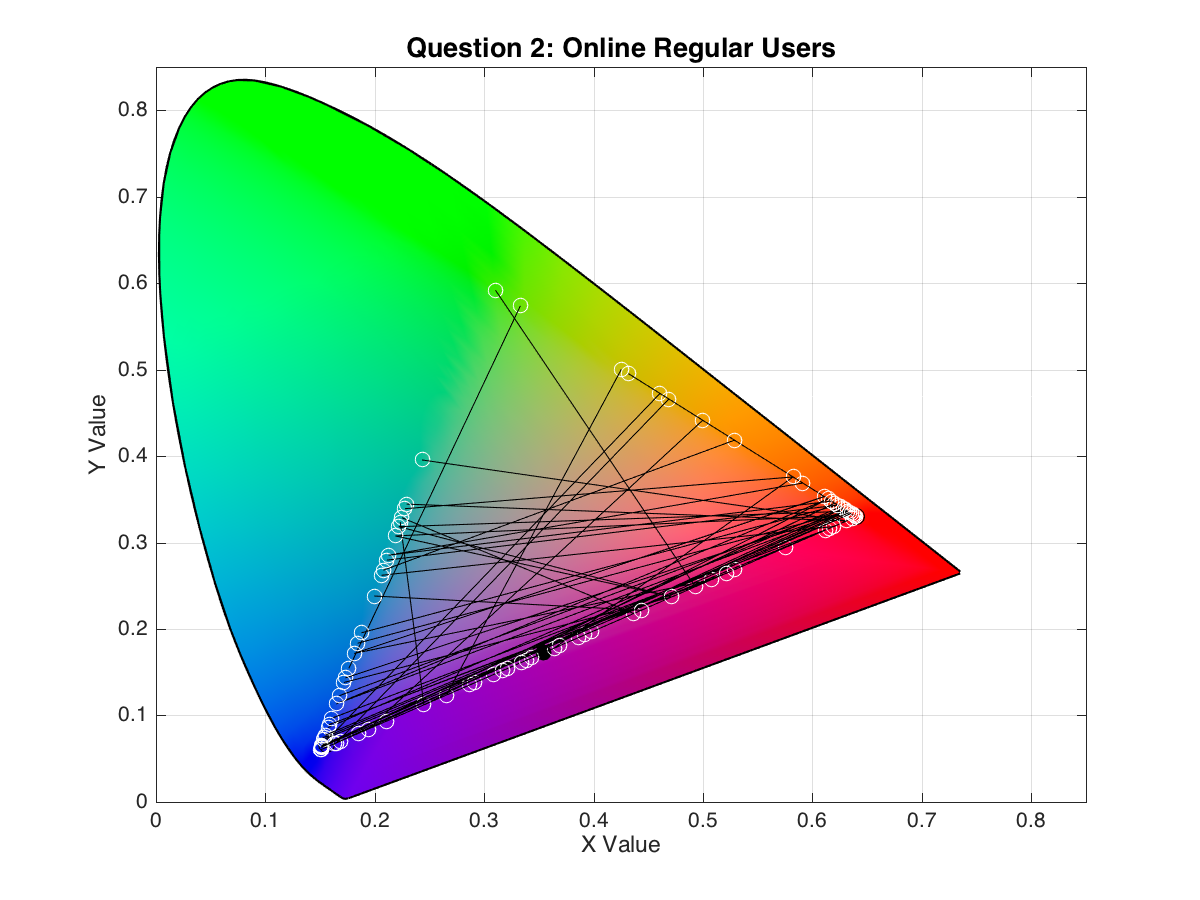
\includegraphics[width=\textwidth]{images/2_online_regularUsers.png}
    \caption[Online Results: Answers for Question 2, from regular users.]{Online Results: Answers for Question 2, from regular users.}
    \label{fig:magentablend_1}
  \end{minipage}\hfill
  \begin{minipage}{0.48\textwidth}
    \centering
    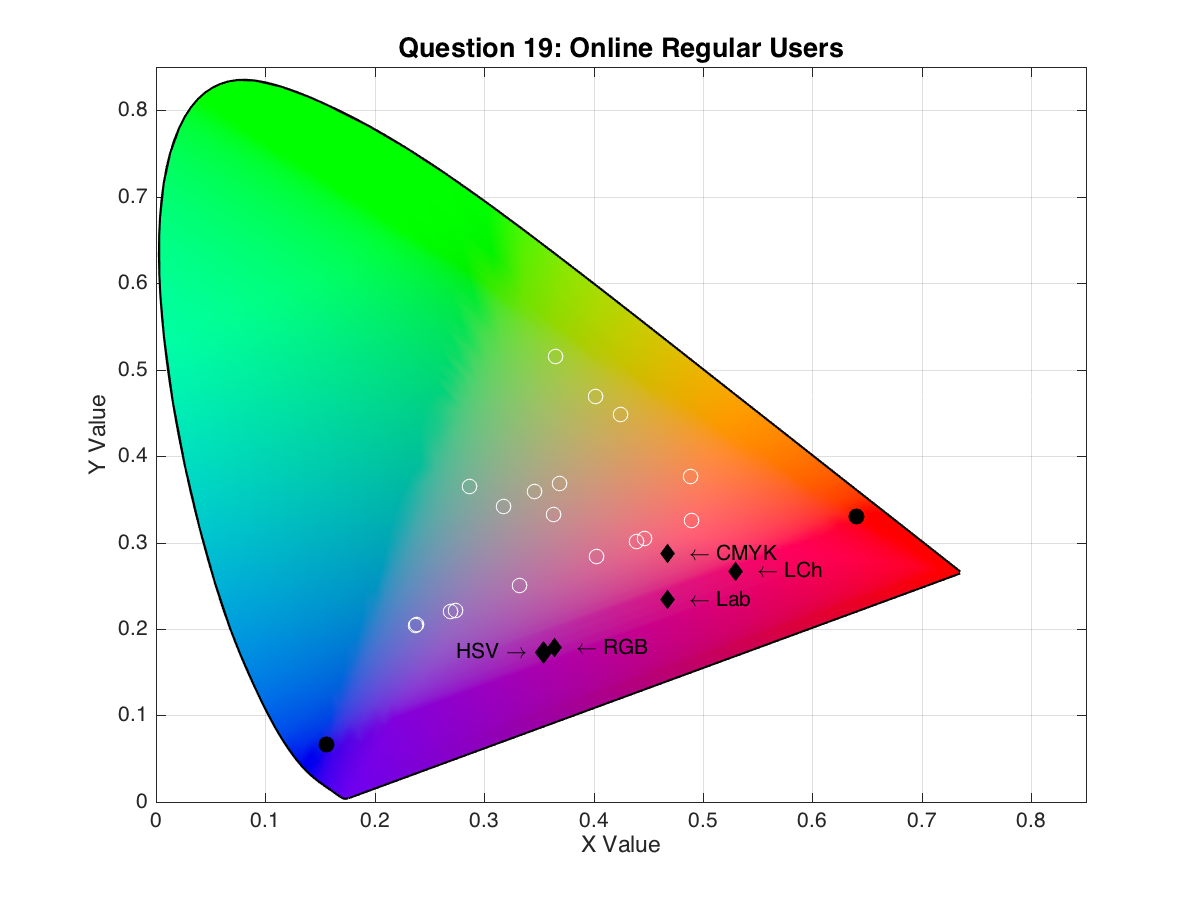
\includegraphics[width=\textwidth]{images/19_online_regularUsers.png}
    \caption[Online Results: Answers for Question 19, from regular users.]{Online Results: Answers for Question 19, from regular users.}
    \label{fig:magentablend_2}
  \end{minipage}
\end{figure}
%
\paragraph{\ul{Red + Green = Yellow}}
%
Lastly, it was expected that users indicate a mixing of Red and Green to mix in a result of Yellow. Both the laboratory and online users provided their answers on similar pairs, comprised between \textbf{blue shades, yellow ones, red and cyan}. There was also an
interesting agregation of results on both environment, \textbf{along the line which unites Blue and Green, and Green and Red}, with a heavy concentration of results near the yellow shades, as seen on Figure \ref{fig:yellowblend_1}. \\
%
The answer-pairs which contained Yellow presented this colors slightly shaded to orange, which could signify that \textbf{the users provided an orangish-yellow with another color in order to blend the first one to the ideal Yellow Hue}. \\
%
Running some descriptive statistics on top of the distance ($\tilde{x} = 0.41$, $\sigma = 0.22$) reveals roughly the same mean distance and standard deviation as before. In this question, the users revealed a balmy concordance amongst themselves, according to color bins
labeling: the users centralized their answers on Blue, Navy-Blue, Orange, Red, Yellow and Green. We could state that \textbf{the users demonstrated some basic conception of blending red and green to obtain yellow}, but further studies should focus on understanting which
influence is the blue color exercising on the user's mental model, since it was a constant result among study environments. \\
%
Analyzing question number eighteen, in which we ask the user which color is the result of blending Red and Green, we conclude that \textbf{the results show an approximation to the ideal color result, but a scattering over orange and yellow colors}.
In this blending, \textbf{there is a slight observable tendency to begin the color blending with a red color}, as depicted in online users' dataset ($20\%$ of fifty-three users) started the mixture with a Red Color. However, this is not a relevant result by itself: it is
indeed consistent with the result collect from the previous mixture. \\
%
\begin{figure}[!htbp]
  \centering
  \begin{minipage}{0.48\textwidth}
    \centering
    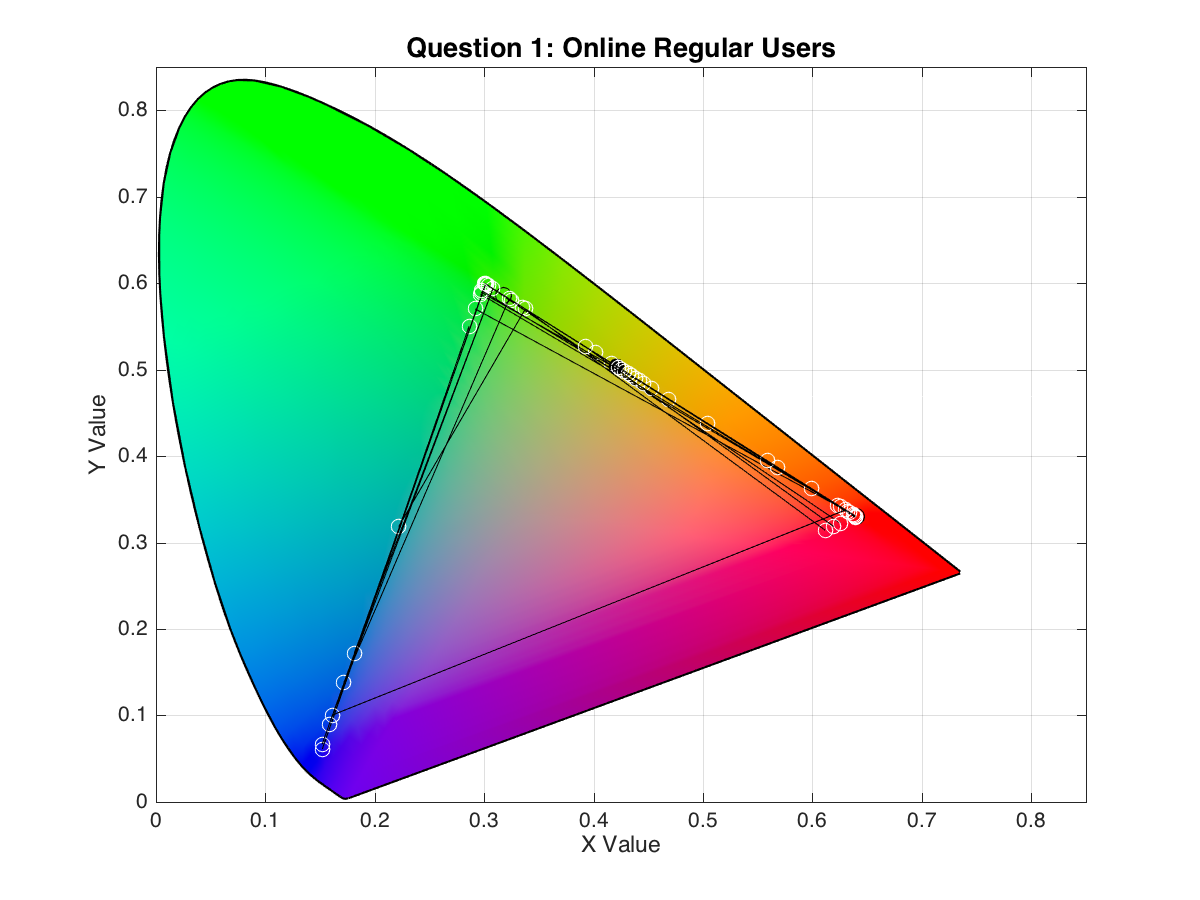
\includegraphics[width=\textwidth]{images/1_online_regularUsers.png}
    \caption[Online Results: Answers for Question 1, from regular users.]{Online Results: Answers for Question 1, from regular users.}
    \label{fig:yellowblend_1}
  \end{minipage}\hfill
  \begin{minipage}{0.48\textwidth}
    \centering
    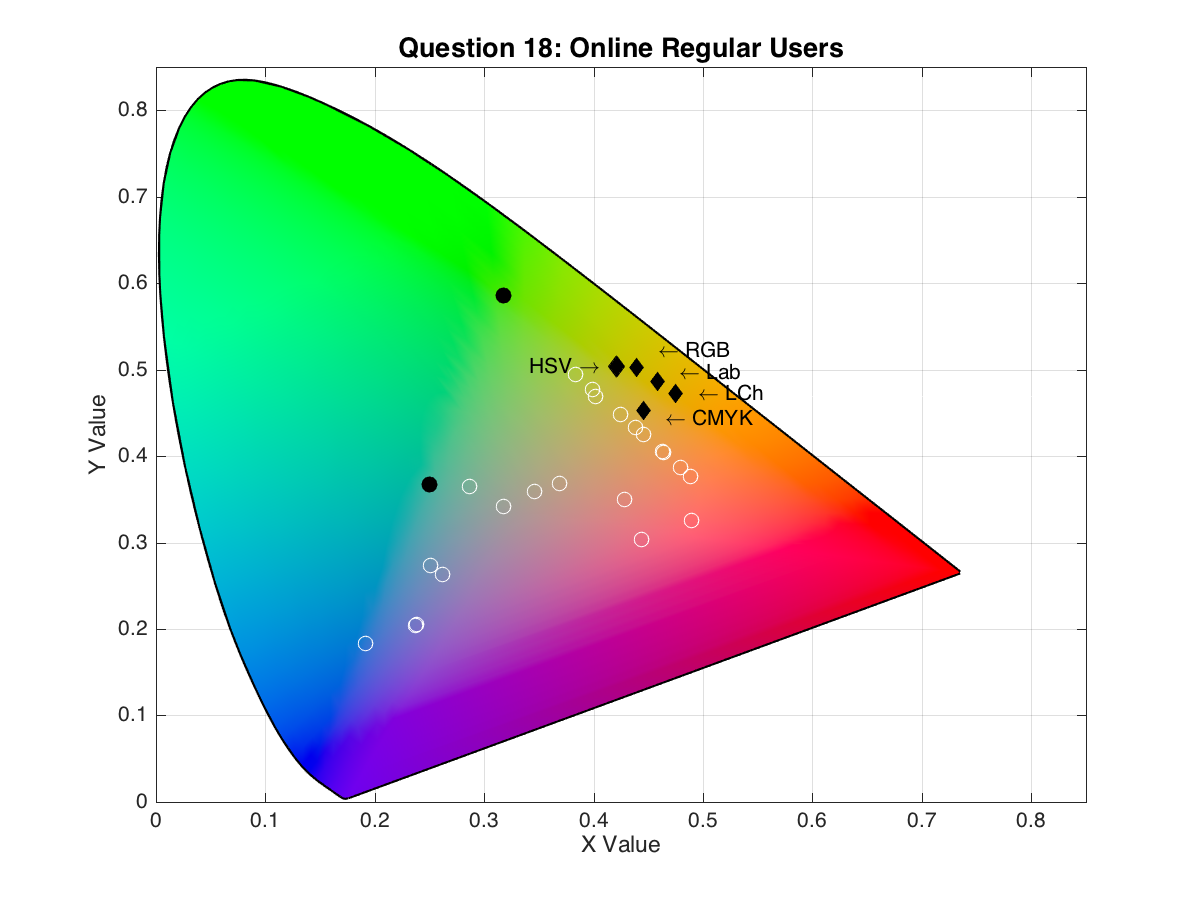
\includegraphics[width=\textwidth]{images/18_online_regularUsers.png}
    \caption[Online Results: Answers for Question 18, from regular users.]{Online Results: Answers for Question 18, from regular users.}
    \label{fig:yellowblend_2}
  \end{minipage}
\end{figure}
%
\subsubsection{Color Blending Effort}
\label{subsubsec:difficulty_rating}
%
Fazer também mistura mais fácil, comparando os ratings das questões e ver qual a mistura que apresenta melhores resultados. \\
Falar de respostas em branco, analisar somente valores e perceber se é desconhecimento. \par
%
Talvez referir aqui novamente, quais foram as misturas com melhores e piores resultados, sem explorar novamente mas apenas para refresh.
%
\subsection{Demographic Results}
\label{subsec:results_demographic}
%
Fazer apenas comparação de faixas etárias entre si, e géneros entre si. \\
Uma ánalise interesse seria comparar faxias etárias por género, mas seria necessária uma amostra bastante mais significativa para cada grupo.
%
\subsubsection{Age Groups}
\label{subsubsec:demo_age}
%
\subsubsection{Gender Groups}
\label{subsubsec:demo_age}
%
\subsubsection{Color Deficient Users Group}
\label{subsubsec:demo_daltonic}
%
%%%%%%%%%%%%%%%%%%%%%%%%%%%%%%%%%%%%%%%%%%%%%%%%%%%%%%%%%%%%%%%%%%%%%%%%%%%%%%%%%%%%%%%%%%%%%%%%%%%%%%%%%%%%%%%%%%%%%%%%%%%%%%%%%%%%%%%%%%%%%%%%%%%
%                                                                DISCUSSION                                                                       %
%%%%%%%%%%%%%%%%%%%%%%%%%%%%%%%%%%%%%%%%%%%%%%%%%%%%%%%%%%%%%%%%%%%%%%%%%%%%%%%%%%%%%%%%%%%%%%%%%%%%%%%%%%%%%%%%%%%%%%%%%%%%%%%%%%%%%%%%%%%%%%%%%%%
%
\section{Discussion}
\label{sec:results_discussion}
%
Fazer apanhado dos resultados todos. \par
abordar questão de que modelos originaram melhores respostas, se são aditivos ou subtrativos. \\
Referir que é preciso estudos para perceber de facto qual é o melhor entre o HSV, Lab e RGB. \\
CMYK claramente melhor \\
LCh claramente pior. \\
%
\subsection{Calibration Resiliency}
\label{subsec:results_calibration}
%
Como verificamos ainda alguns users com calibração imprópria para teste, considerámos que poderia ser uma fonte de resultados
interessantes. Como tal, criámos um dataset para os mesmos e comparámos com os resultados dos utilizadores calibrados. Os resultados
são os que se seguem... \par
%
\subsection{Creation of Color Scales}
\label{subsec:results_discussion_colorscales}
%
Aproveitar resultado de respostas em branco
%
\subsection{Color Organization}
\label{subsec:results_discussion_colororganization}

\subsection{Implications for InfoVis}
\label{subsec:results_discussion_infovis}
%
Resumo dos resultados todos e regras que se podem levar deste trabalho para a área de InfoVis em geral.
%
